\documentclass[12pt]{article}
\usepackage[english]{babel}
\usepackage[utf8]{inputenc}
\usepackage{helvet}
\usepackage{graphicx}
\usepackage{longtable}
\usepackage{multirow}
\usepackage[unicode=true, hidelinks]{hyperref}
\setlength{\parindent}{0pt}
\setlength{\parskip}{6pt plus 2pt minus 1pt}
\setcounter{secnumdepth}{4}
\usepackage{array}
\usepackage{float}

\newcommand{\plogo}{\fbox{$\mathcal{PL}$}} % Generic dummy publisher logo

\usepackage[utf8]{inputenc} % Required for inputting international characters
\usepackage[T1]{fontenc} % Output font encoding for international characters
%\usepackage{fouriernc} % Use the New Century Schoolbook font

\renewcommand{\listtablename}{Tables}
\graphicspath{ {./images/} }

%\title{
%\textbf{
%{\fontsize{30}{104}\selectfont Software Specification Requirement}
%\\* For
%\\* {\fontsize{30}{104}\selectfont Digital Board Marker}
%}
%}
%\date{\vspace{-5ex}}


\begin{document}
%\maketitle
%\begin{flushright}
%\textbf{Prepared by:}
%\vspace{0.5cm}
%\\* \textbf{Muhammad Haris Khan, Hamza Farooq, Ayesha Atif, Komal Shehzadi}
%\vspace{0.5cm}
%\\* \textbf{Department of Computer Science and Engineering, UET Lahore.}
%\end{flushright}

\begin{titlepage} % Suppresses headers and footers on the title page

	\centering % Centre everything on the title page
	
	\scshape % Use small caps for all text on the title page
	
	\vspace*{\baselineskip} % White space at the top of the page
	
	%------------------------------------------------
	%	Title
	%------------------------------------------------
	
	\rule{\textwidth}{1.6pt}\vspace*{-\baselineskip}\vspace*{2pt} % Thick horizontal rule
	\rule{\textwidth}{0.4pt} % Thin horizontal rule
	
	\vspace{0.75\baselineskip} % Whitespace above the title
	
	{\LARGE Software Requirement Specification\\ For\\ Digital Board Marker\\} % Title
	
	\vspace{0.75\baselineskip} % Whitespace below the title
	
	\rule{\textwidth}{0.4pt}\vspace*{-\baselineskip}\vspace{3.2pt} % Thin horizontal rule
	\rule{\textwidth}{1.6pt} % Thick horizontal rule
	
	\vspace{2\baselineskip} % Whitespace after the title block
	
	%------------------------------------------------
	%	Subtitle
	%------------------------------------------------
	

	Version 3.0
	
	\vspace*{3\baselineskip} % Whitespace under the subtitle
	
	%------------------------------------------------
	%	Editor(s)
	%------------------------------------------------
	
	Prepared By
	
	\vspace{0.5\baselineskip} % Whitespace before the editors
	
	{ Muhammad Haris Khan(2016-CS-105) \\ Hamza Farooq(2016-CS-122) \\ Ayesha Atif(2016-CS-152) \\ Komal Shehzadi(2016-CS-178)} % Editor list
	
	\vspace{0.5\baselineskip} % Whitespace below the editor list
	
	\textit{University of Engineering and Technology \\ Lahore} % Editor affiliation
	
	\vfill % Whitespace between editor names and publisher logo
	
	%------------------------------------------------
	%	Publisher
	%------------------------------------------------
	
	
	
	\vspace{0.3\baselineskip} % Whitespace under the publisher logo
	
	\textit{Copyright \textsuperscript{\textcopyright} 2019 all rights reserved} % Publication year
	


\end{titlepage}


\tableofcontents

\listoffigures
 
\listoftables


\newpage


\section{Introduction}

\subsection{Background}
Digital Board Marker is a size efficient, bandwidth saving lecture recording system. It can record lecture, providing automated google search of handwritten words. It provides on the spot wiki. Lecture text notes can be generated automatically. Lecture can be named and divided into topics and subtopics automatically. According to a survey, 94\% students go for online help of recently attended lectures because they can’t fully grab the concepts. Recorded lectures as video format require so much internet bandwidth to play. In most cases, large sized videos are difficult to handle or download. Because students mostly don’t have huge amount of extra space available especially for the CSE students, as they already use bulky software and also students don’t have large amount of bandwidth of internet available.
Digital Board Marker is an innovation and need of the hour because it is solving the basic problem of all students in society because it saves their time to note the lecture and they can concentrate on the topic completely. As most of the student lost their concentration while writing the detailed lecture. Moreover, sometimes we skip important part of our lecture in the effort of writing whole details on our notebook. So, Digitized Lecture System is leading-edge to solve all these Issues. It has some potential for having positive effect on student learning.
\subsection{Motivation}
The motivation and purpose to do this project is to minimize the use of resources that are used in lecture systems now a days working in all over the world i.e. video lecture recording and streaming through internet. The first motivation is to deal with the large amount of storage that normally video lectures take. This system is not based on video recording but on recording the writing on the board with marker. It will record the position of the marker as the coordinates of board where marker touches and store it in the text file (which will later be converted and played like a video). This will take minimum amount of database storage to store this kind of data on a website. The second motivation to do this project is to use less internet resources for accessing the lectures. Normally the video lectures of different institutes worldwide are very large and to download those on the system through internet requires large amount of resources which are normally difficult for students to get and to download it in high quality even more resources are required. The lectures for recording are very low in memory as compared to normal video recording and will require very minimum resources to download on the system. The third motivation is for example a power failure occurred during the lecture and you cannot clearly see the board but teacher is still writing and erases the board after some time, this may result in not getting proper notes or missing the important point of lecture. Moreover students can get benefit by seeing the lecture again and again if they missed any concept or if they were absent minded or not attending lecture. These few are the reasons which motivated us to do this project.



\subsection{Scope}
Digital board marker mainly cover academic area the main purpose is to provide each and every student all the lectures with better quality and less bandwidth because in Pakistan we students face this issue the most, as we know it cannot be resolved in near future we have to work something out for this issue and that’s where this system will work it will provide an interface to all the students which have all the lectures of their respective subjects from their respective teachers which can be streamed online and downloaded for offline to play later on at very low bandwidth. It will provide all the assignment related material and lectures at same platform to students. It is the new revolution in the academic field. Although it covers industry and researches as well.

\subsection{Problem Statement}
To make a storage and bandwidth efficient system with a lecture player and learning management system for the students and the educational institutes.

\subsection{Application Areas}
\subsubsection{Educational Institutes:}
Educational institutes can use digital board marker for online lectures. They can have different users:
\begin{itemize}
\item Admin
\item Teacher
\item Student
\end{itemize}
\subsubsection{Online Tutors}
Online tutors can use the system to deliver lectures online with high quality and low storage. Tutor can login and start recording lecture, upload and delete them. Students/Listeners can play and download the lectures.
\subsubsection{Sketch Artists}
Sketch artists can give online tutorials of sketching with high quality video and less storage use for users. User can play video again and again without using much data.



\section{Existing Work}

\subsection{Details of Existing Work}
Online video lecture systems that exist now a days are:\\
\begin{itemize}
\item Edx
\item Coursera
\item Udemy
\item Udacity
\end{itemize}
These are the system which are very helpful to users and can be accessed by everyone. They provide video lectures of class recording the video and audio. Almost all the systems
use this same procedure of recording with camera and microphone.

\subsection{Comparison of Existing Work}
\begin{figure}[h]
  \centering
  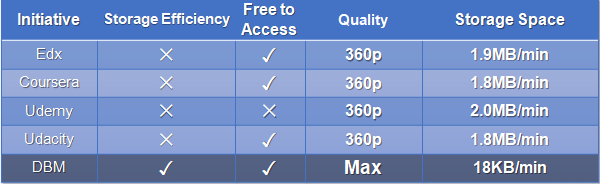
\includegraphics[width=14cm, height=5cm]{ExistingSystemsTable}
  \caption{Existing Systems}
\end{figure}

%\subsection{Product Functions}
%\subsubsection{Desktop and Mobile Application}
%
%\begin{flushleft}
%\textbf{Files:}
%\begin{itemize}
%\item Open: Loads an existing Lecture file.
%\item Open Recent: Loads one of the displayed, recently opened Lecture files.
%\item Properties: Displays some properties of the Lecture (such as the title, duration and number of topic tags) which can be edited.
%\item Save: Saves the edited lecture file without changing its name or directory.
%\item Save as: Saves the lecture file and gives the user the ability to change its name or directory.
%\item Exit: DBM app shuts down
%\end{itemize}
%\end{flushleft}
%
%\begin{flushleft}
%\textbf{Player Window:}
%\begin{itemize}
%\item Resize: Resize the application player view window.
%\item Play/Pause: Plays or Pauses the lecture animation.
%\item Audio control: Controls the audio level.
%\item Next: Play next lecture in lecture playlist.
%\item Previous: Play previous lecture in lecture playlist.
%\item Fast Forward: Speeds up lecture animation and audio track as well.
%\item Slow down: Slower the animation speed and also audio track.
%\item Timeline: Displays the timeline tab.
%\end{itemize}
%\end{flushleft}
%
%\begin{flushleft}
%\textbf{Splash Screens:}
%\begin{itemize}
%\item Welcome: Displays the Welcome window.
%\end{itemize}
%\end{flushleft}
%
%\begin{flushleft}
%\textbf{Help:}
%\begin{itemize}
%\item Check for Updates: Displays the plugins that can be updated to newer versions
%\item About: Displays the logo of DBM, which licenses are being used, the product version and other info.
%\end{itemize}
%\end{flushleft}
%
%\subsubsection{Web Application}
%\begin{flushleft}
%
%
%\textbf{Main Page:}
%\begin{itemize}
%\item Login/Registration: Displays the Login and Registration pages in which students as well as teachers or instructors can be registered and login afterwards.
%\item Course Section: Displays all available courses to student and instructor.
%\item Lectures Section: Includes lecture hierarchy and lecture player.
%\end{itemize}
%\end{flushleft}
%
%\begin{flushleft}
%\textbf{Login/Registration:}
%\begin{itemize}
%\item Registration Page: Requests First name, Last name, CNIC, Degree, Email, Country, Education institution, Password from user being registered and sends a verification email.
%\item Login Page: Require Username and password from user.
%\end{itemize}
%\end{flushleft}
%
%\begin{flushleft}
%\textbf{Course Section:}
%\begin{itemize}
%\item All Courses Page: Includes all available courses and display them to the respective user or instructor.
%\item Registered Courses: Displays the courses in which current user is registered.
%\end{itemize}
%\end{flushleft}
%
%\begin{flushleft}
%\textbf{Lecture Hierarchy:}
%\begin{itemize}
%\item Course Content Page: Lectures and the corresponding date.
%\item Configuration: Preferences about how the data is presented.
%\item Add Lecture: Manage recently recorded unlisted lectures.
%\item Search: Stand Search functionality.
%\end{itemize}
%\end{flushleft}
%
%
%\begin{flushleft}
%\textbf{Lecture Player:}
%\begin{itemize}
%\item Resize: Resize the application player view window.
%\item Play/Pause: Plays or Pauses the lecture animation.
%\item Audio control: Controls the audio level.
%\item Next: Play next lecture in lecture playlist.
%\item Previous: Play previous lecture in lecture playlist.
%\item Fast Forward: Speeds up lecture animation and audio track as well.
%\item Slow down: Slower the animation speed and also audio track.
%\item Timeline: Displays the timeline tab.
%\end{itemize}
%\end{flushleft}
%
%\begin{flushleft}
%\textbf{Splash Screens:}
%\begin{itemize}
%\item Welcome: Displays the Welcome window.
%\end{itemize}
%\end{flushleft}
%
%\begin{flushleft}
%\textbf{Active Learning Control Panel:}
%\begin{itemize}
%\item how controls such as on/off and other button controls under this panel.
%\end{itemize}
%\end{flushleft}
%
%\subsection{User Classes and Characteristics}
%
%\begin{itemize}
%\item Typical Users, such as students, who want to use DBM for watching online lectures as well as download to view it in offline mode later after.
%\item Professional Users, such as Instructors or teachers who want to use DBM for editing and annotations.
%\end{itemize}
%
%
%\subsection{Operating Environment}
%
%\begin{itemize}
%\item Windows 7
%\item Windows 8
%\item Windows 10
%\item Android 4.0 and higher
%\item Web Browser with HTML5
%\end{itemize}
%
%
%\subsection{Design and Implementation Constraints}
%DBM is developed in C Sharp, it uses .net Core as build platform of web application. Desktop application is developed in C Sharp as well. It is developed as windows form application in visual studio 2015. Android app is developed in Android studio that features editing and annotation of video lecture and requires name, category and course name of the currently being uploaded lecture.
%
%\subsection{User Documentation}
%There is a quick start guide available on the website of DBM
%
%\subsection{Assumptions and Dependencies}
%DBM web app is developed in C Sharp visual studio 2015. Web application requires any browser that supports HTML5 and CSS3. Supported browsers are Chrome, Safari, Firefox latest version.
%DBM desktop app is developed as windows form application in visual C Sharp. It requires some runtime libraries to be installed on client’s machine such as:
%\begin{itemize}
%\item Visual Redistributables
%\item .Net Framework 4.5
%\end{itemize}

\section{Software Development Life Cycle}
\subsection{SDLC Used}
The SDLC model used is Agile model.
Agile SDLC model is a combination of iterative and incremental process models with focus on process adaptability and customer satisfaction by rapid delivery of working software product. Agile Methods break the product into small incremental builds. These builds are provided in iterations.\\
Each iteration typically lasts from about one to three weeks. Every iteration involves cross functional teams working simultaneously on various areas like:
\begin{itemize}
\item Planning
\item Requirements Analysis
\item Design
\item Coding
\item Unit Testing and
\item Acceptance Testing
\end{itemize}

At the end of the iteration, a working product is displayed to the customer and important stakeholders.\\
Agile model believes that every project needs to be handled differently and the existing methods need to be tailored to best suit the project requirements. In Agile, the tasks are divided to time boxes (small time frames) to deliver specific features for a release. Iterative approach is taken and working software build is delivered after each iteration. Each build is incremental in terms of features; the final build holds all the features required by the customer.\\

\subsection{Justification for SDLC}
In our project at first requirements were not so clear so we opted for agile model where while working on current requirements we plan next phase easily.
At first we worked on waterfall model then analysing the system we have decided to work with agile model because it is most suitable. There are three separate modules working right now. Each module is developing in iteration which is considered to be one week. Each week one person is scrum master who arranges daily group meetings in which we discuss the problems in previous assigned tasks and how to solve them, approach to be taken in coming week tasks.

\section{Requirement Analysis}
\subsection{Functional Requirements}
\begin{itemize}
\item User should be able to register and login.
\item Student should be able to view a course and enrol in the course.
\item Admin should be able to add new course.
\item Teacher should be able to see student's enrolment requests.
\item Admin should be able to see teacher's and students' registration requests and approve them.
\item All user should be able to view and download the lecture.
\item Teacher should be able to delete a lecture.
\item Users should be able to download course notes.
\item Teacher should be able to add new course notes.
\item Students should be able to download and submit assignments.
\item Teacher should be able to add new assignment and download all students' assignments.
\item User should be able to play lectures.
\item Admin should be able to add new permissions, user groups and assign permissions to users.

\end{itemize}

\subsection{Non-functional Requirements}
\subsubsection{Performance Requirements}
Some performance requirements are listed below.
\begin{itemize}
\item The software should support the use of multiple users at a time.
\item The database should be able to record thousands of records.
\item Live streaming of lecture should also be possible within low bandwidth.
\item Software should support the live streaming of multiple lectures at a time.
\item No loss of data should occur while uploading the lecture.
\item No loss of data should occur while live streaming of lecture.
\end{itemize}
%
%


\subsubsection{Security Requirements}
Some of the factors that are identified to protect the software from accidental and malicious attacks are discussed below.
\begin{itemize}
\item Assign certain function to different modules.
\item Check data integrity for critical variables.
\end{itemize}

\subsubsection{Software Quality Attributes}
\begin{itemize}
\item \textbf{Availability:} The system should be available on any time for use of multiple users.
\item \textbf{Correctness:} The system should provide correct content and lectures of a specific subject.
\item \textbf{Usability:} The system should satisfy a maximum number of user needs.
\item \textbf{Confidentiality:} Software should allow only authorized users to access the System.
\item \textbf{Portability:} Software should be portable to avoid any problem that may occur from moving one OS to another OS.
\item \textbf{Supportability:} Software should use proper naming conventions and coding standards.
\end{itemize}



\newpage
%\section{External Interface Requirements}
\subsection{User Interfaces (Web App)}
\subsubsection{Main page}
\begin{figure}[h]
  \centering
  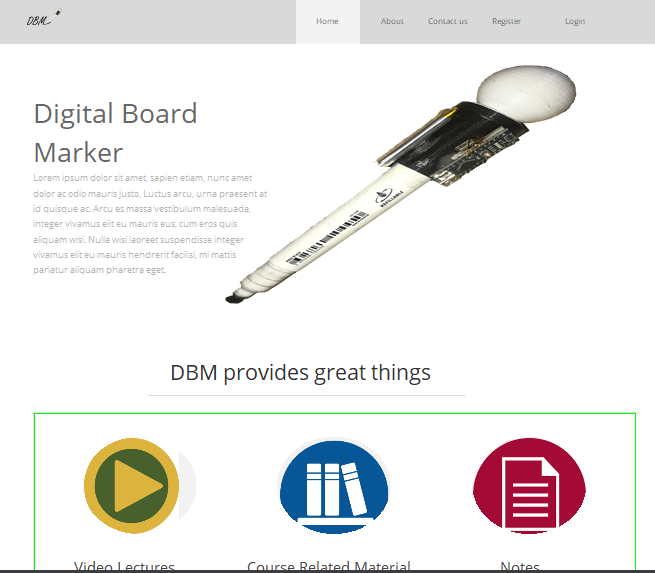
\includegraphics[width=10cm, height=10cm]{MainPage(1)}
  \caption{Main Page}
\end{figure}
\newpage
\begin{figure}[h]
  \centering
  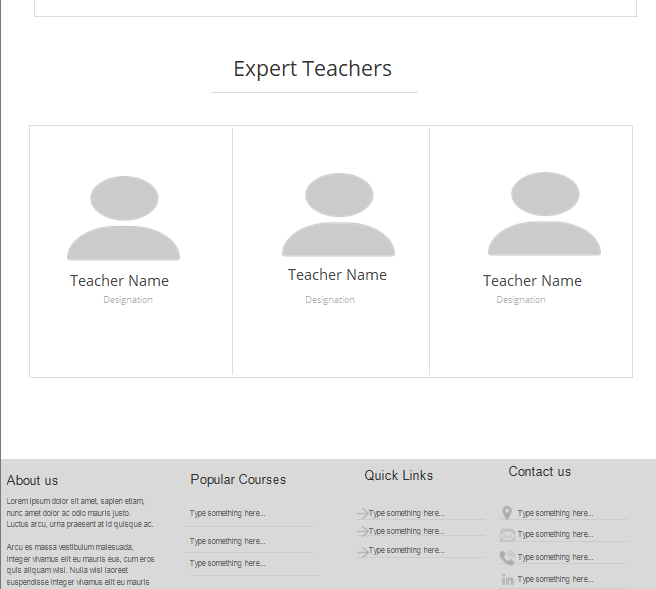
\includegraphics[width=10cm, height=10cm]{MainPage(2)}
  \caption{Main Page}
\end{figure}

\begin{longtable}{|p{2cm}|p{4cm}|p{4cm}|p{4cm}|}
\hline
\textbf{Tasks} & \textbf{As an Admin} & \textbf{As a Teacher} & \textbf{As a Student}\\
\hline
% Row 1 start
T1 &
I shall be able to see register page &
I shall be able to see register page &
I shall be able to see register page \\
% Row 1 end
\hline

% Row 2 start
T2 &
I shall be able to see login page &
I shall be able to see login page &
I shall be able to see login page \\
% Row 2 end
\hline

% Row 3 start
T3 &
I shall be able to manage permissions page & & \\
% Row 3 end
\hline

% Row 4 start
T4 &
I shall be able to manage courses page & & \\
% Row 4 end
\hline

% Row 5 start
T5 &
I shall be able to see all institutes page & & \\
% Row 5 end
\hline

% Row 6 start
T6 &
I shall be able to manage all teachers page & & \\
% Row 6 end
\hline
\caption{Main Page}
\end{longtable}



%\begin{figure}[h]
%  \centering
%  \begin{minipage}[b]{0.3\textwidth}
%    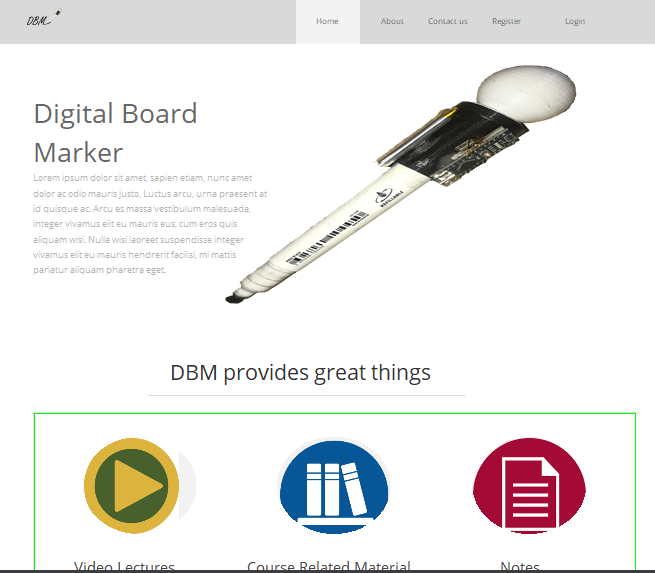
\includegraphics[width=\textwidth]{MainPage(1)}
%    \caption{Main Page}
%  \end{minipage}
%  \hfill
%  \begin{minipage}[b]{0.3\textwidth}
%    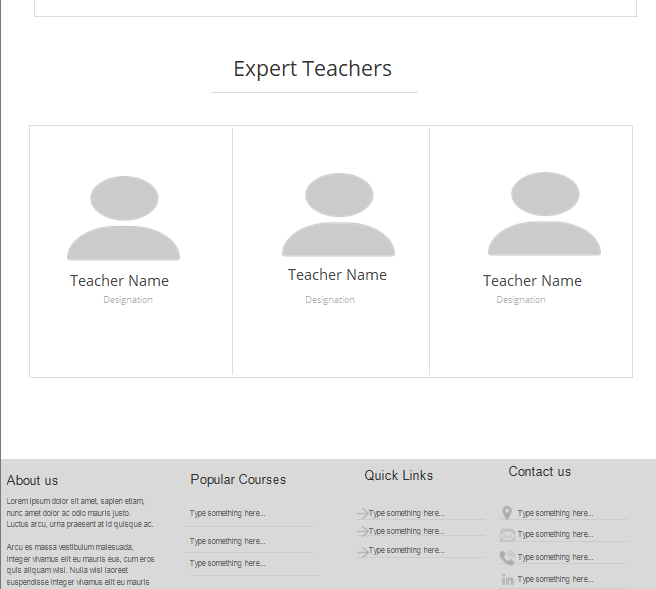
\includegraphics[width=\textwidth]{MainPage(2)}
%    \caption{Main Page}
%  \end{minipage}
%\end{figure}




\subsubsection{Registration page}
\begin{figure}[h]
  \centering
  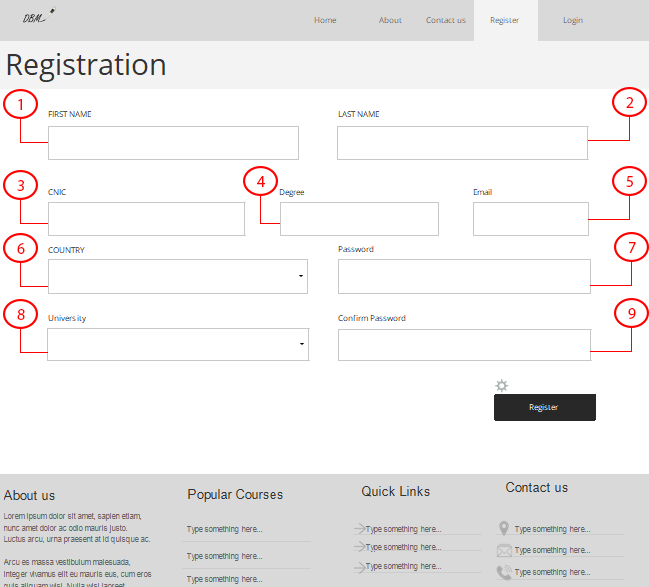
\includegraphics[width=10cm, height=10cm]{RegistrationPage}
  \caption{Registration}
\end{figure}

\begin{longtable}{|>{\raggedright\arraybackslash}p{2.5cm}|>{\raggedright\arraybackslash}p{2.5cm}|>{\raggedright\arraybackslash}p{2.5cm}|>{\raggedright\arraybackslash}p{2cm}|>{\raggedright\arraybackslash}p{2cm}|}
\hline
\textbf{Component} & \textbf{Description} & \textbf{Mandatory} & \textbf{Validation} & \textbf{Type}\\
\hline
% Row 1 start
1 &
First name of user. &
Yes &
Only letters &
string \\
% Row 1 end
\hline

% Row 2 start
2 &
Last name of user. &
Yes &
Only letters &
string \\
% Row 2 end
\hline

% Row 3 start
3 &
CNIC number of user. &
Yes &
16 digit number &
string \\
% Row 3 end
\hline

% Row 4 start
4 &
Designation of user. &
Yes &
Only letters &
string \\
% Row 4 end
\hline

% Row 5 start
5 &
Email of user. &
Yes &
Email format &
string \\
% Row 5 end
\hline

% Row 6 start
6 &
Country of user. &
Yes &
Only letters &
string \\
% Row 6 end
\hline


% Row 7 start
7 &
Password of user. &
Yes &
Only letters &
string \\
% Row 7 end
\hline

% Row 8 start
8 &
University name of user. &
Yes &
Only letters &
string \\
% Row 8 end
\hline

% Row 9 start
9 &
Re-Enter password of user. &
Yes &
Only letters &
string \\
% Row 9 end
\hline

\caption{Registration}
\end{longtable}

\subsubsection{Login page}
\begin{figure}[H]
  \centering
  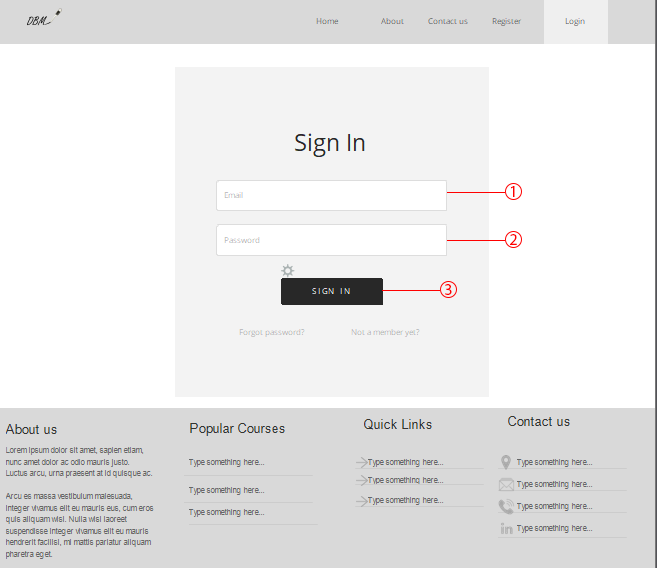
\includegraphics[width=9cm, height=9cm]{Login}
  \caption{Login}
\end{figure}

\newpage
\begin{longtable}{|>{\raggedright\arraybackslash}p{2.5cm}|>{\raggedright\arraybackslash}p{2.5cm}|>{\raggedright\arraybackslash}p{2.5cm}|>{\raggedright\arraybackslash}p{2cm}|>{\raggedright\arraybackslash}p{2cm}|}
\hline
\textbf{Component} & \textbf{Description} & \textbf{Mandatory} & \textbf{Validation} & \textbf{Type}\\
\hline
% Row 1 start
1 &
User registered email. &
Yes &
Email format. &
string \\
% Row 1 end
\hline

% Row 2 start
2 &
User password corresponding to email. &
Yes &
None &
string \\
% Row 2 end
\hline

% Row 3 start
3 &
Sign in button to login to account and perform actions. &
Yes &
None &
submit \\
% Row 3 end
\hline

\caption{Login}
\end{longtable}


%\subsubsection{All Courses page(Student)}
%After log in user can see all the courses uploaded.
%\begin{figure}[h]
%  \centering
%  \includegraphics[width=6cm, height=6cm]{AllCoursespage(Student)}
%  \caption{Course page(Student)}
%\end{figure}



\subsubsection{All Courses}
\begin{figure}[H]
  \centering
  \includegraphics[width=8cm, height=7.5cm]{AllCoursespage(Teacher)}
  \caption{Course page}
\end{figure}
\begin{longtable}{|>{\raggedright\arraybackslash}p{2.5cm}|>{\raggedright\arraybackslash}p{2.5cm}|>{\raggedright\arraybackslash}p{2.5cm}|>{\raggedright\arraybackslash}p{2cm}|>{\raggedright\arraybackslash}p{2cm}|}
\hline
\textbf{Component} & \textbf{Description} & \textbf{Mandatory} & \textbf{Validation} & \textbf{Type}\\
\hline
% Row 1 start
1 &
To view details of courses. &
None &
None &
None 
\\
% Row 1 end
\hline

% Row 2 start
2 &
To delete a course from list. &
None &
None &
None 
\\
% Row 2 end
\hline

% Row 3 start
3 &
Search box to search course from the list. &
None &
None &
None 
\\
% Row 3 end
\hline

% Row 4 start
4 &
Button to add new courses. &
None &
None &
None 
\\
% Row 4 end
\hline

\caption{All Courses}
\end{longtable}



\subsubsection{Add Courses page}
\begin{figure}[h]
  \centering
  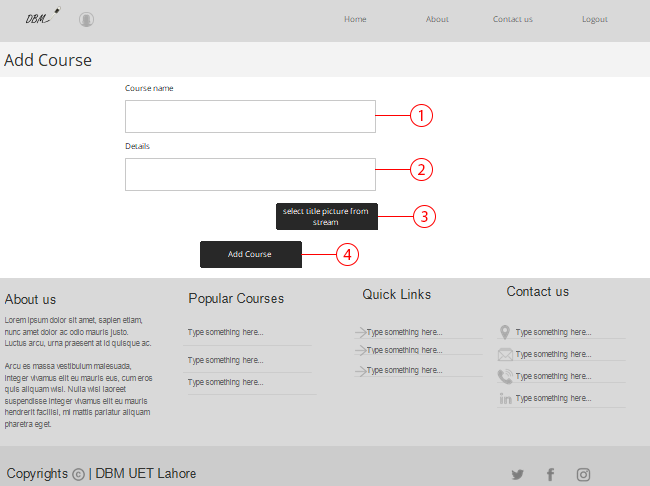
\includegraphics[width=10cm, height=8cm]{AddNewCourse}
  \caption{Add Course Page}
\end{figure}

\begin{longtable}{|>{\raggedright\arraybackslash}p{2.5cm}|>{\raggedright\arraybackslash}p{2.5cm}|>{\raggedright\arraybackslash}p{2.5cm}|>{\raggedright\arraybackslash}p{2cm}|>{\raggedright\arraybackslash}p{2cm}|}
\hline
\textbf{Component} & \textbf{Description} & \textbf{Mandatory} & \textbf{Validation} & \textbf{Type}\\
\hline
% Row 1 start
1 &
Name of the course. &
Yes &
None &
string\\
% Row 1 end
\hline

% Row 2 start
2 &
Description related to course. &
Yes &
None &
string \\
% Row 2 end
\hline

% Row 3 start
3 &
Button to add title image for course. &
No &
None &
Submit \\
% Row 3 end
\hline

% Row 4 start
4 &
Save button to save course in database. &
None &
None &
None \\
% Row 4 end
\hline

\caption{Add Courses}
\end{longtable}



\subsubsection{Courses Details}
\begin{figure}[h]
  \centering
  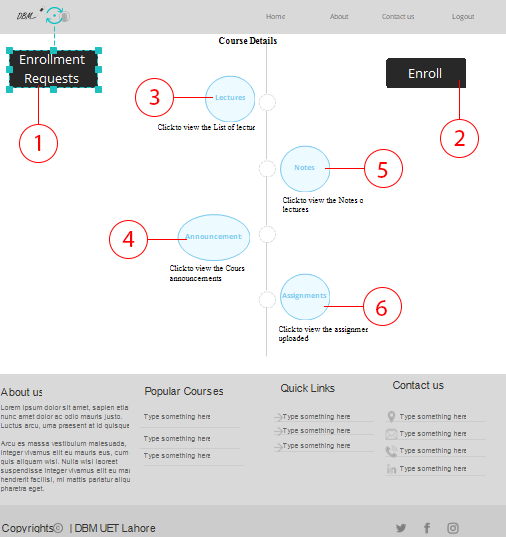
\includegraphics[width=12cm, height=8cm]{CourseDetails}
  \caption{Course Details}
\end{figure}

\newpage

\begin{longtable}{|>{\raggedright\arraybackslash}p{2.5cm}|>{\raggedright\arraybackslash}p{2.5cm}|>{\raggedright\arraybackslash}p{2.5cm}|>{\raggedright\arraybackslash}p{2cm}|>{\raggedright\arraybackslash}p{2cm}|}
\hline
\textbf{Component} & \textbf{Description} & \textbf{Mandatory} & \textbf{Validation} & \textbf{Type}\\
\hline
% Row 1 start
1 &
To see enrolment request of students in course. It will be only visible to teacher. &
None &
None &
None\\
% Row 1 end
\hline

% Row 2 start
2 &
To enrol in course. It will be only visible to students. &
None&
None &
None \\
% Row 2 end
\hline

% Row 3 start
3 &
To see list of all video lectures. &
None &
None &
None \\
% Row 3 end
\hline

% Row 4 start
4 &
To see list of announcements. &
None &
None &
None \\
% Row 4 end
\hline

% Row 5 start
5 &
To see list of notes. &
None &
None &
None \\
% Row 5 end
\hline

% Row 6 start
6 &
To see list of assignments. &
None &
None &
None \\
% Row 6 end
\hline

\caption{Courses Details}
\end{longtable}


\newpage
\subsubsection{Teachers Registration Requests}
\begin{figure}[h]
  \centering
  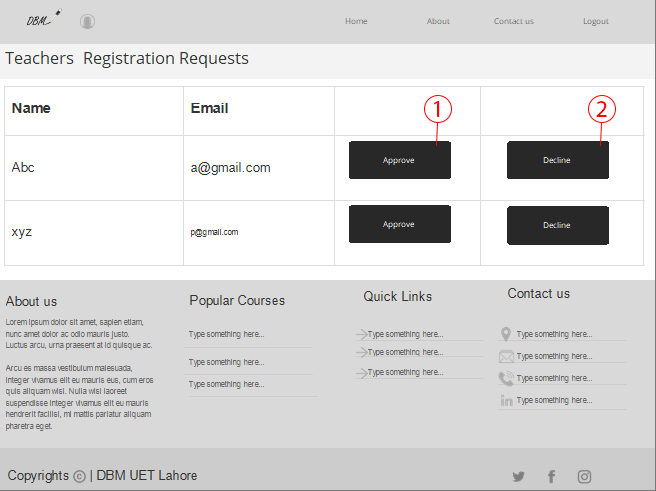
\includegraphics[width=10cm, height=10cm]{TeachersRegistrationRequests}
  \caption{Teachers Registration Requests Page}
\end{figure}

\begin{longtable}{|>{\raggedright\arraybackslash}p{2.5cm}|>{\raggedright\arraybackslash}p{2.5cm}|>{\raggedright\arraybackslash}p{2.5cm}|>{\raggedright\arraybackslash}p{2cm}|>{\raggedright\arraybackslash}p{2cm}|}
\hline
\textbf{Component} & \textbf{Description} & \textbf{Mandatory} & \textbf{Validation} & \textbf{Type}\\
\hline
% Row 1 start
1 &
To approve teachers registration requests. This will only be visible to admin. &
None &
None &
None\\
% Row 1 end
\hline

% Row 2 start
2 &
To delete teachers registration requests. This will only be visible to admin. &
None &
None &
None \\
% Row 2 end
\hline

\caption{Teachers Registration Requests}
\end{longtable}



\subsubsection{Students Registration Requests}
\begin{figure}[H]
  \centering
  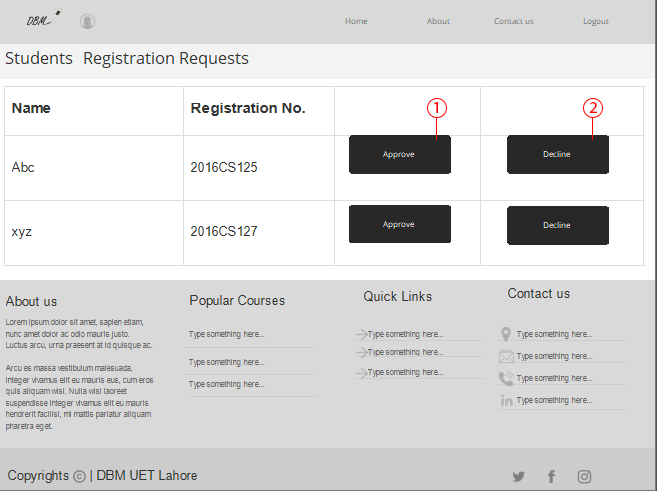
\includegraphics[width=9cm, height=9cm]{StudentsRegistrationRequests}
  \caption{Students Registration Requests Page}
\end{figure}

\newpage
\begin{longtable}{|>{\raggedright\arraybackslash}p{2.5cm}|>{\raggedright\arraybackslash}p{4cm}|>{\raggedright\arraybackslash}p{2.2cm}|>{\raggedright\arraybackslash}p{2cm}|>{\raggedright\arraybackslash}p{2cm}|}
\hline
\textbf{Component} & \textbf{Description} & \textbf{Mandatory} & \textbf{Validation} & \textbf{Type}\\
\hline
% Row 1 start
1 &
To approve students registration requests. This will only be visible to admin. &
None &
None &
None\\
% Row 1 end
\hline

% Row 2 start
2 &
To delete students registration requests. This will only be visible to admin. &
None &
None &
None \\
% Row 2 end
\hline

\caption{Students Registration Requests}
\end{longtable}


\subsubsection{Enrollment Requests}
\begin{figure}[h]
  \centering
  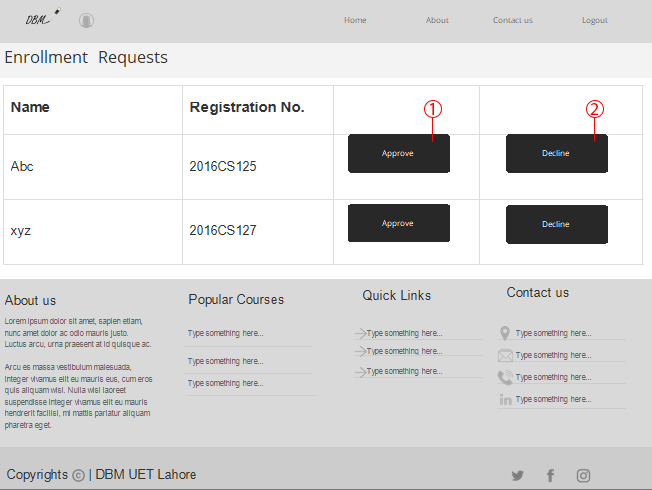
\includegraphics[width=9cm, height=9cm]{EnrollmentRequests}
  \caption{Enrollment Requests}
\end{figure}

\newpage
\begin{longtable}{|>{\raggedright\arraybackslash}p{2.5cm}|>{\raggedright\arraybackslash}p{4cm}|>{\raggedright\arraybackslash}p{2.2cm}|>{\raggedright\arraybackslash}p{2cm}|>{\raggedright\arraybackslash}p{2cm}|}
\hline
\textbf{Component} & \textbf{Description} & \textbf{Mandatory} & \textbf{Validation} & \textbf{Type}\\
\hline
% Row 1 start
1 &
To approve students enrolment requests. This will only be visible to admin. &
None &
None &
None\\
% Row 1 end
\hline

% Row 2 start
2 &
To delete students enrolment requests. This will only be visible to admin. &
None &
None &
None \\
% Row 2 end
\hline

\caption{Enrollment Requests}
\end{longtable}



\subsubsection{Lecture Details}
\begin{figure}[H]
  \centering
  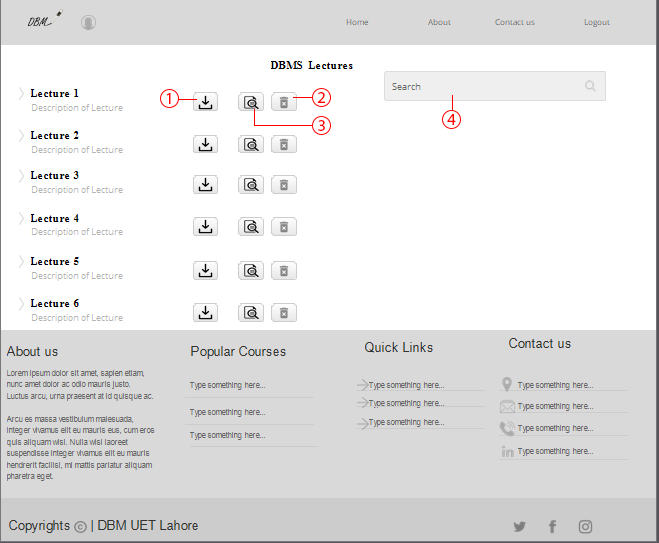
\includegraphics[width=9cm, height=9cm]{LectureDetails(Teacher)}
  \caption{Lecture Details(Teacher)}
\end{figure}

\newpage

\begin{longtable}{|>{\raggedright\arraybackslash}p{2.5cm}|>{\raggedright\arraybackslash}p{4cm}|>{\raggedright\arraybackslash}p{2.2cm}|>{\raggedright\arraybackslash}p{2cm}|>{\raggedright\arraybackslash}p{2cm}|}
\hline
\textbf{Component} & \textbf{Description} & \textbf{Mandatory} & \textbf{Validation} & \textbf{Type}\\
\hline
% Row 1 start
1 &
To download the lecture file. &
None &
None &
None\\
% Row 1 end
\hline

% Row 2 start
2 &
To delete the lecture. This will be only visible to teacher. &
None &
None &
None \\
% Row 2 end
\hline

% Row 3 start
3 &
To play lecture online. &
None &
None &
None \\
% Row 3 end
\hline

% Row 4 start
4 &
A search box to search for lectures from list. &
None &
None &
None \\
% Row 4 end
\hline

\caption{Lecture Detials}
\end{longtable}

%\subsubsection{Lecture Details(Student)}
%Student can see all the lectures and can play the lectures from list.
%\begin{figure}[h]
%  \centering
%  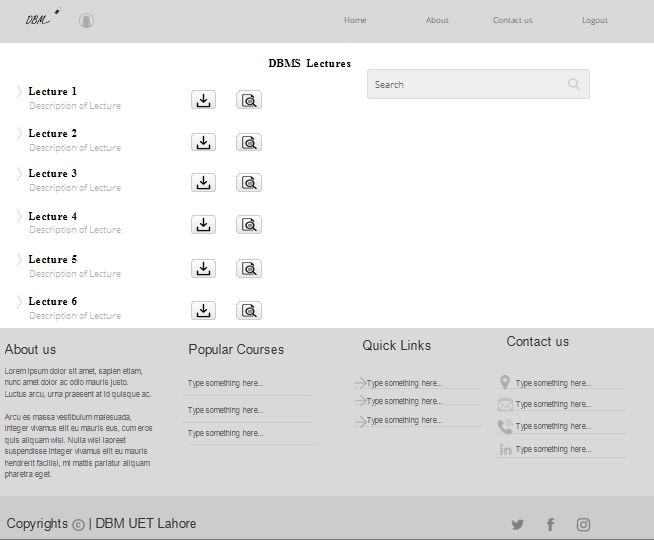
\includegraphics[width=6cm, height=6cm]{LectureDetails(Student)}
%  \caption{Lecture Details(Student)}
%\end{figure}



%\subsubsection{Notes(Student)}
%Student can see all the notes uploaded by teacher.
%\begin{figure}[h]
%  \centering
%  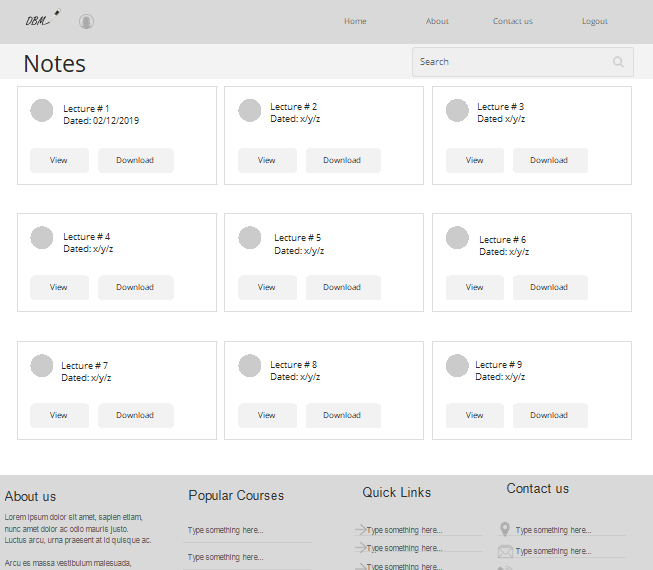
\includegraphics[width=6cm, height=6cm]{NotesPage(Student)}
%  \caption{Notes(For Students)}
%\end{figure}
%
%
%
\subsubsection{Notes}
\begin{figure}[h]
  \centering
  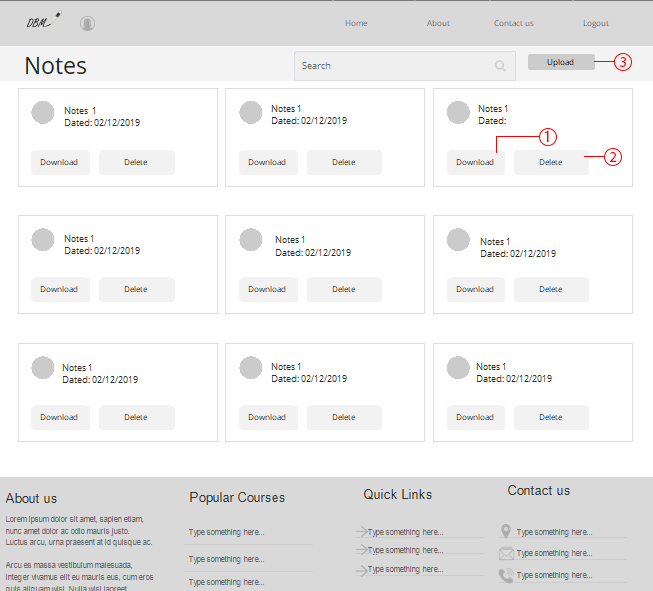
\includegraphics[width=9cm, height=9cm]{NotesPage(Teacher)}
  \caption{Notes}
\end{figure}

\newpage
\begin{longtable}{|>{\raggedright\arraybackslash}p{2.5cm}|>{\raggedright\arraybackslash}p{4cm}|>{\raggedright\arraybackslash}p{2.2cm}|>{\raggedright\arraybackslash}p{2cm}|>{\raggedright\arraybackslash}p{2cm}|}
\hline
\textbf{Component} & \textbf{Description} & \textbf{Mandatory} & \textbf{Validation} & \textbf{Type}\\
\hline
% Row 1 start
1 &
To download the notes file. &
None &
None &
None\\
% Row 1 end
\hline

% Row 2 start
2 &
To delete the lecture. This will be only visible to teacher. &
None &
None &
None \\
% Row 2 end
\hline

% Row 3 start
3 &
To upload new notes file. This will be only visible to teacher. &
None &
None &
None \\
% Row 3 end
\hline

\caption{Notes}
\end{longtable}


\subsubsection{Upload Notes}
\begin{figure}[H]
  \centering
  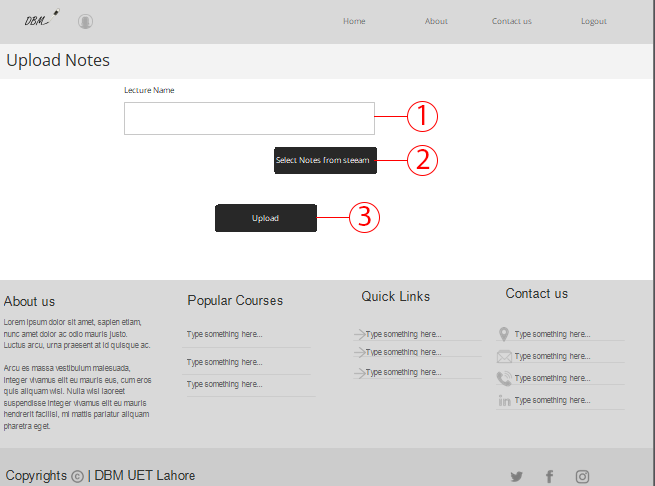
\includegraphics[width=9cm, height=9cm]{UploadNotesPage}
  \caption{Upload Notes}
\end{figure}

\newpage
\begin{longtable}{|>{\raggedright\arraybackslash}p{2.5cm}|>{\raggedright\arraybackslash}p{4cm}|>{\raggedright\arraybackslash}p{2.2cm}|>{\raggedright\arraybackslash}p{2cm}|>{\raggedright\arraybackslash}p{2cm}|}
\hline
\textbf{Component} & \textbf{Description} & \textbf{Mandatory} & \textbf{Validation} & \textbf{Type}\\
\hline
% Row 1 start
1 &
Title for notes file name. &
Yes &
None &
string \\
% Row 1 end
\hline

% Row 2 start
2 &
To upload notes file. &
Yes &
None &
None \\
% Row 2 end
\hline

% Row 3 start
3 &
Upload button to save the data. &
None &
None &
None \\
% Row 3 end
\hline

\caption{Add Notes}
\end{longtable}



%\subsubsection{Course Content(Student)}
%Student can see all the course content like book, can download them.
%\begin{figure}[h]
%  \centering
%  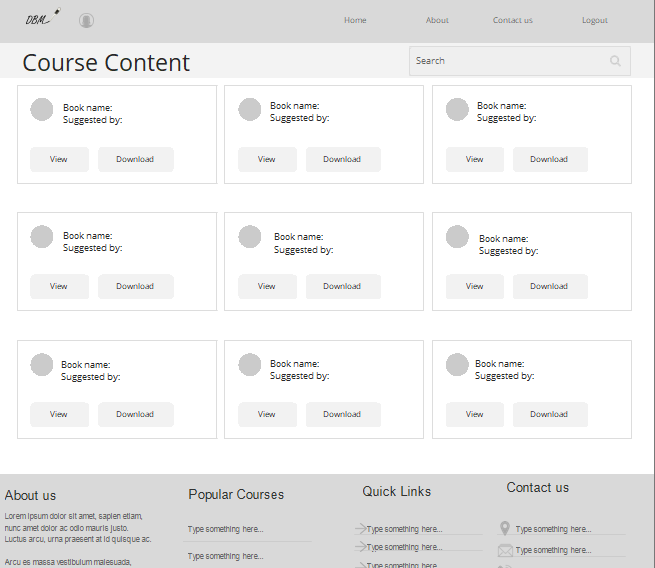
\includegraphics[width=6cm, height=6cm]{CourseContentPage(Student)}
%  \caption{Course Content(For Student)}
%\end{figure}
%
%
%\subsubsection{Course Content(Teacher)}
%Teacher can see all the course content(books, slides), can remove and upload more content.
%\begin{figure}[h]
%  \centering
%  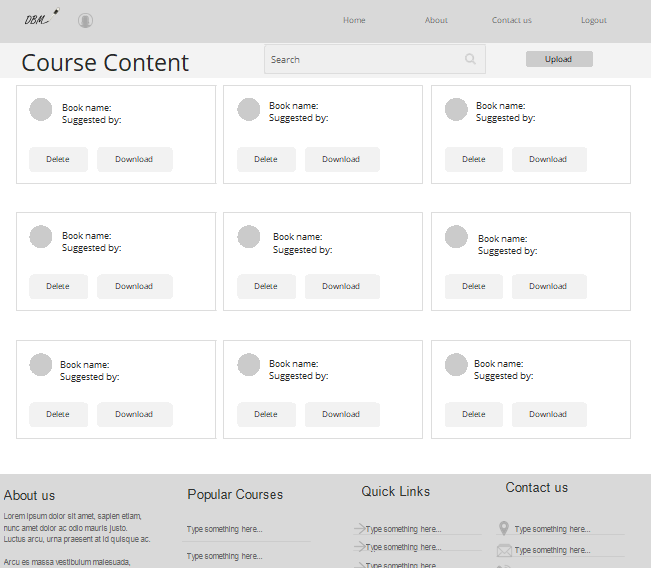
\includegraphics[width=6cm, height=6cm]{CourseContentPage(Teacher)}
%  \caption{Course Content(For Teacher)}
%\end{figure}
%
%
%\subsubsection{Upload Course Content}
%Teacher can see all the course content(books, slides), can remove and upload more content.
%\begin{figure}[h]
%  \centering
%  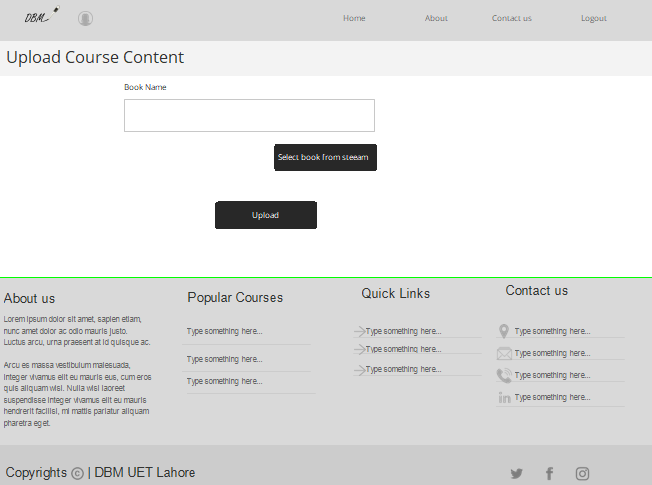
\includegraphics[width=6cm, height=6cm]{UploadCourseContent}
%  \caption{Upload Course Content}
%\end{figure}
%
%
%\subsubsection{Course Assignment(Student)}
%Student can see all the assignments, can download the assignments.
%\begin{figure}[h]
%  \centering
%  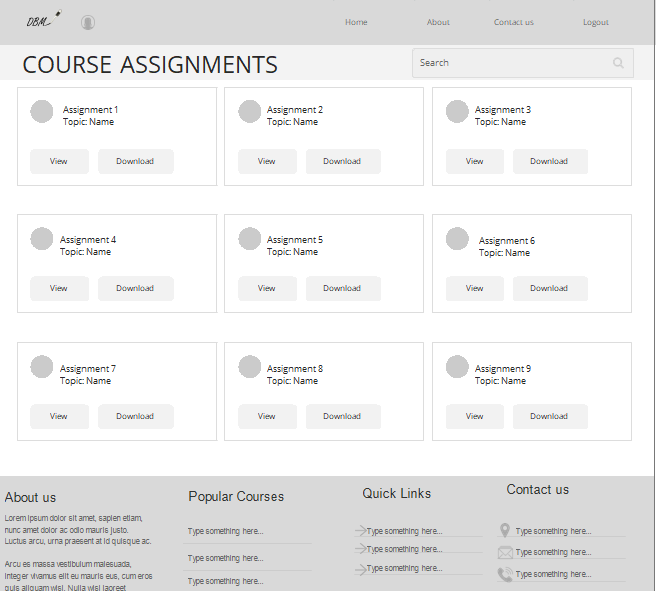
\includegraphics[width=6cm, height=6cm]{CourseAssignmentPage(Student)}
%  \caption{Course Assignments(For Student)}
%\end{figure}
%
%
\subsubsection{Course Assignment}
\begin{figure}[H]
  \centering
  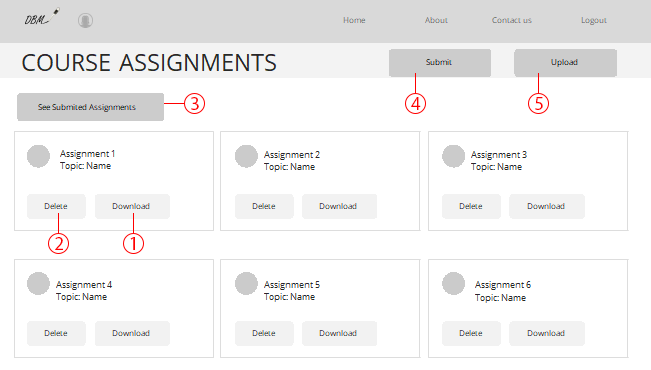
\includegraphics[width=9cm, height=9cm]{CourseAssignmentPage(Teacher)}
  \caption{Course Assignments}
\end{figure}
\begin{longtable}{|>{\raggedright\arraybackslash}p{2.5cm}|>{\raggedright\arraybackslash}p{4cm}|>{\raggedright\arraybackslash}p{2.2cm}|>{\raggedright\arraybackslash}p{2cm}|>{\raggedright\arraybackslash}p{2cm}|}
\hline
\textbf{Component} & \textbf{Description} & \textbf{Mandatory} & \textbf{Validation} & \textbf{Type}\\
\hline
% Row 1 start
1 &
To download assignment file. &
None &
None &
None \\
% Row 1 end
\hline

% Row 2 start
2 &
To delete assignment file. This will be only visible to teacher. &
None &
None &
None \\
% Row 2 end
\hline

% Row 3 start
3 &
To see all the submitted assignments. &
None &
None &
None \\
% Row 3 end
\hline

% Row 4 start
4 &
To submit any assignment. This will be only visible to students. &
None &
None &
None \\
% Row 4 end
\hline

% Row 5 start
5 &
To upload new assignment. This will be only visible to teacher. &
None &
None &
None \\
% Row 5 end
\hline

\caption{Assignments}
\end{longtable}


%SubmitAssignment
\subsubsection{Submit Assignment}
\begin{figure}[h]
  \centering
  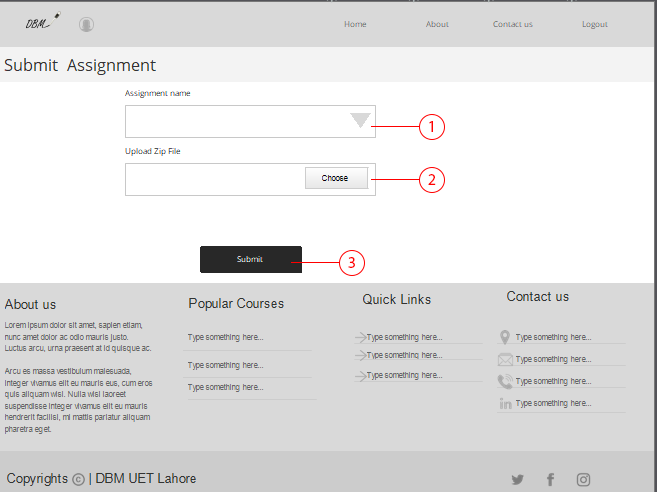
\includegraphics[width=9cm, height=7cm]{SubmitAssignment}
  \caption{Submit Assignments}
\end{figure}

\newpage
\begin{longtable}{|>{\raggedright\arraybackslash}p{2.5cm}|>{\raggedright\arraybackslash}p{4cm}|>{\raggedright\arraybackslash}p{2.2cm}|>{\raggedright\arraybackslash}p{2cm}|>{\raggedright\arraybackslash}p{2cm}|}
\hline
\textbf{Component} & \textbf{Description} & \textbf{Mandatory} & \textbf{Validation} & \textbf{Type}\\
\hline
% Row 1 start
1 &
Select assignment name student want to submit. &
Yes &
None &
string \\
% Row 1 end
\hline

% Row 2 start
2 &
Choose assignment file to be submitted. &
Yes &
None &
None \\
% Row 2 end
\hline

% Row 3 start
3 &
To submit assignment and save in database. &
None &
None &
None \\
% Row 3 end
\hline


\caption{Submit Assignments}
\end{longtable}


\subsubsection{Submitted Assignment}
\begin{figure}[H]
  \centering
  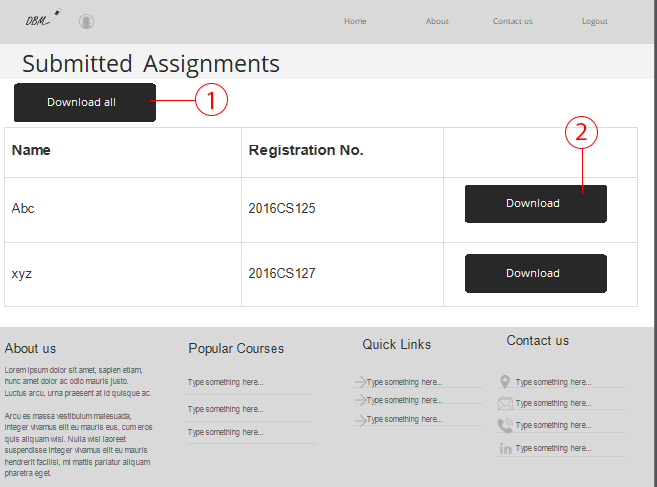
\includegraphics[width=9cm, height=9cm]{SubmittedAssignments}
  \caption{Submitted Assignments}
\end{figure}

\newpage
\begin{longtable}{|>{\raggedright\arraybackslash}p{2.5cm}|>{\raggedright\arraybackslash}p{4cm}|>{\raggedright\arraybackslash}p{2.2cm}|>{\raggedright\arraybackslash}p{2cm}|>{\raggedright\arraybackslash}p{2cm}|}
\hline
\textbf{Component} & \textbf{Description} & \textbf{Mandatory} & \textbf{Validation} & \textbf{Type}\\
\hline
% Row 1 start
1 &
To download all students assignments. &
None &
None &
None \\
% Row 1 end
\hline

% Row 2 start
2 &
To download individual assignments. &
None &
None &
None \\
% Row 2 end
\hline


\caption{All Submitted Assignments}
\end{longtable}


\subsubsection{Upload Assignment}
\begin{figure}[H]
  \centering
  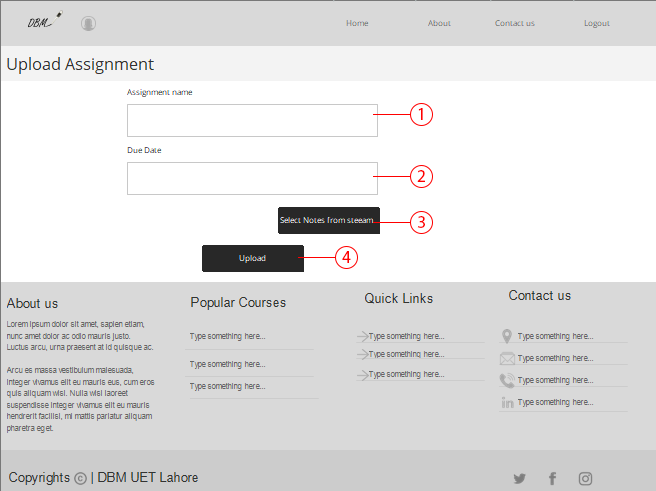
\includegraphics[width=10cm, height=10cm]{UploadAssignmentsPage}
  \caption{Upload Assignments}
\end{figure}

\newpage
\begin{longtable}{|>{\raggedright\arraybackslash}p{2.5cm}|>{\raggedright\arraybackslash}p{4cm}|>{\raggedright\arraybackslash}p{2.2cm}|>{\raggedright\arraybackslash}p{2cm}|>{\raggedright\arraybackslash}p{2cm}|}
\hline
\textbf{Component} & \textbf{Description} & \textbf{Mandatory} & \textbf{Validation} & \textbf{Type}\\
\hline
% Row 1 start
1 &
Title of assignment file. &
Yes &
None &
None \\
% Row 1 end
\hline

% Row 2 start
2 &
Due date to submit assignment. &
Yes &
Date format &
Date \\
% Row 2 end
\hline

% Row 3 start
3 &
To assignment file. &
None &
None &
None \\
% Row 3 end
\hline

% Row 4 start
4 &
To save data in database. &
None &
None &
None \\
% Row 4 end
\hline

\caption{Add Assignments}
\end{longtable}


%\subsubsection{All Classes Page}
%\begin{figure}[h]
%  \centering
%  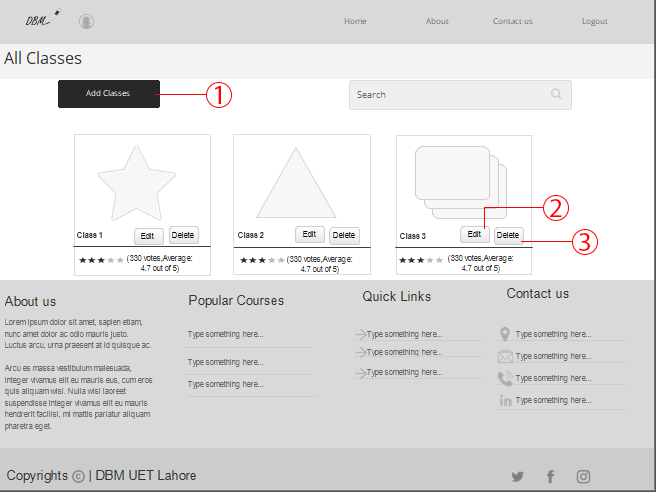
\includegraphics[width=9cm, height=9cm]{AllClassesPage}
%  \caption{All Classes added}
%\end{figure}
%
%\newpage
%\begin{longtable}{|p{2cm}|p{13cm}|}
%\hline
%\textbf{Tasks} & \textbf{As an Admin}\\
%\hline
%% Row 1 start
%T1 &
%I shall be able to see all classes.
%\\
%% Row 1 end
%\hline
%
%% Row 2 start
%T2 &
%I shall be able go to edit class page.
%\\
%% Row 2 end
%\hline
%
%% Row 3 start
%T3 &
%I shall be able go to class.
%\\
%% Row 3 end
%\hline
%
%\caption{All Classes}
%\end{longtable}


%\newpage
%\subsubsection{Edit Classes Page}
%\begin{figure}[h]
%  \centering
%  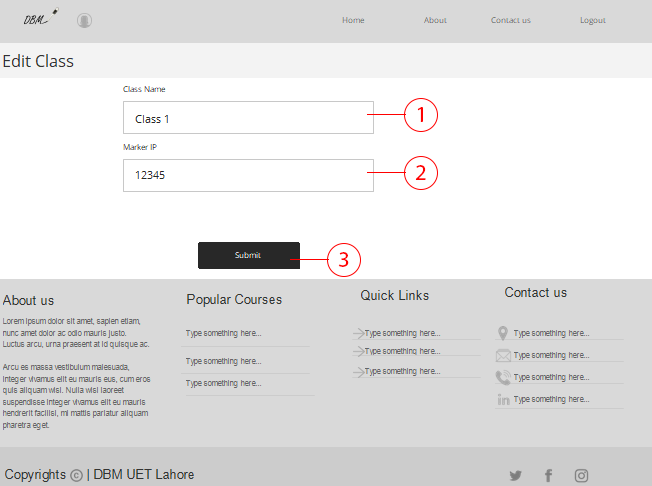
\includegraphics[width=12cm, height=12cm]{EditClassPage}
%  \caption{Edit Class}
%\end{figure}
%\begin{longtable}{|p{2cm}|p{13cm}|}
%\hline
%\textbf{Tasks} & \textbf{As an Admin}\\
%\hline
%% Row 1 start
%T1 &
%I shall be able to edit class name and marker IP.
%\\
%% Row 1 end
%\hline
%
%\caption{Edit Class}
%\end{longtable}


%\newpage
%
%\subsubsection{Add New Class Page}
%\begin{figure}[h]
%  \centering
%  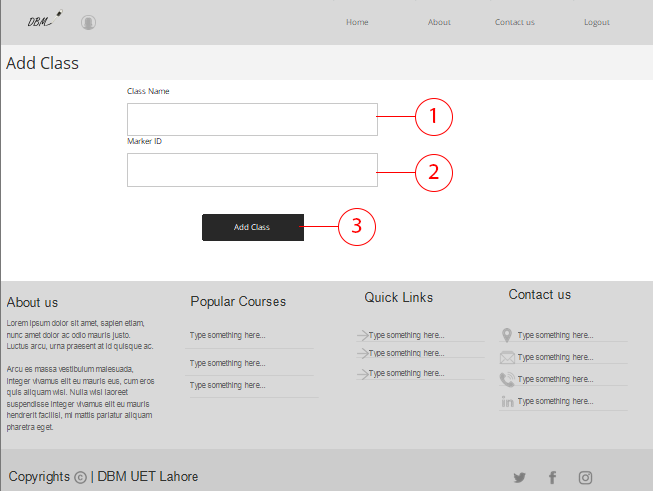
\includegraphics[width=12cm, height=13cm]{AddClassesPage(Teacher)}
%  \caption{Add new classes}
%\end{figure}
%\begin{longtable}{|p{2cm}|p{13cm}|}
%\hline
%\textbf{Tasks} & \textbf{As an Admin}\\
%\hline
%% Row 1 start
%T1 &
%I shall be able to add new classes.
%\\
%% Row 1 end
%\hline
%\caption{Add Classes}
%\end{longtable}


\subsubsection{Lecture Player}
\begin{figure}[H]
  \centering
  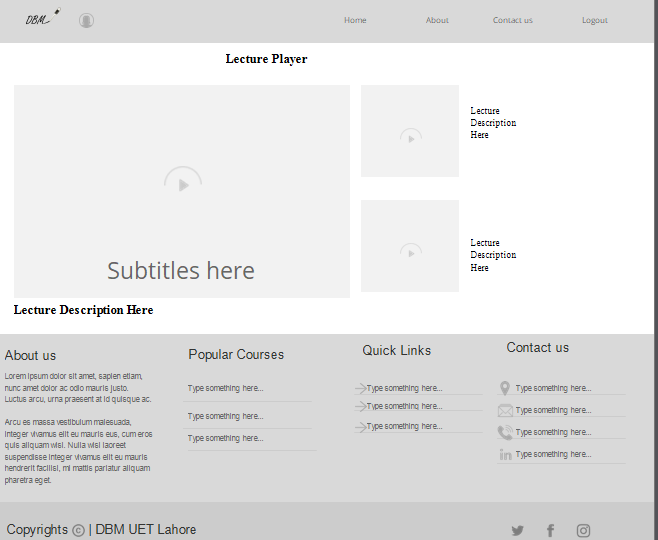
\includegraphics[width=10cm, height=10cm]{LecturePlayer}
  \caption{Play Lecture}
\end{figure}
\newpage
\begin{longtable}{|p{2cm}|p{4cm}|p{4cm}|p{4cm}|}
\hline
\textbf{Tasks} & \textbf{As an Admin} & \textbf{As a Teacher} & \textbf{As a Student}\\
\hline
% Row 1 start
T1 &
I shall be able to play lecture on video player. &
I shall be able to play lecture on video player. &
I shall be able to play lecture on video player.
\\
% Row 1 end
\hline
\caption{Lecture Player}
\end{longtable}
%
%\newpage
%
%\subsubsection{Start Lecture}
%\begin{figure}[h]
%  \centering
%  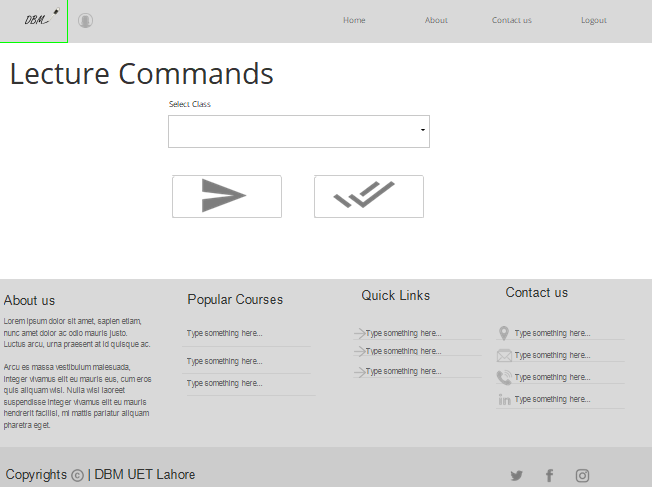
\includegraphics[width=12cm, height=13cm]{PlayLecture(Start)}
%  \caption{Lecture Start}
%\end{figure}
%\begin{longtable}{|p{2cm}|p{13cm}|}
%\hline
%\textbf{Tasks} & \textbf{As a Teacher}\\
%\hline
%% Row 1 start
%T1 &
%I shall be able to start lecture from the class.
%\\
%% Row 1 end
%\hline
%\caption{Start Lecture}
%\end{longtable}
%
%\newpage

\subsubsection{Student Details}
\begin{figure}[H]
  \centering
  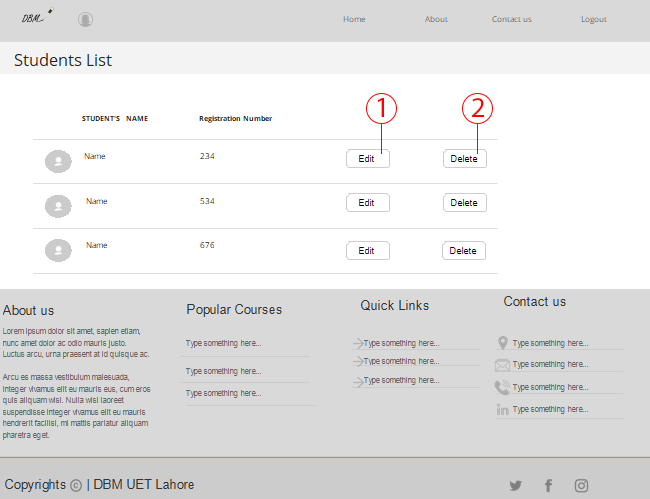
\includegraphics[width=9cm, height=9cm]{StudentDetails(Admin)}
  \caption{Student Details}
\end{figure}

\begin{longtable}{|>{\raggedright\arraybackslash}p{2.5cm}|>{\raggedright\arraybackslash}p{4cm}|>{\raggedright\arraybackslash}p{2.2cm}|>{\raggedright\arraybackslash}p{2cm}|>{\raggedright\arraybackslash}p{2cm}|}
\hline
\textbf{Component} & \textbf{Description} & \textbf{Mandatory} & \textbf{Validation} & \textbf{Type}\\
\hline
% Row 1 start
1 &
To edit the student details. &
None &
None &
None \\
% Row 1 end
\hline

% Row 2 start
2 &
To remove the student from record. &
None &
None &
None \\
% Row 2 end
\hline

\caption{Student Details}
\end{longtable}

\newpage

\subsubsection{Teacher Details}
\begin{figure}[h]
  \centering
  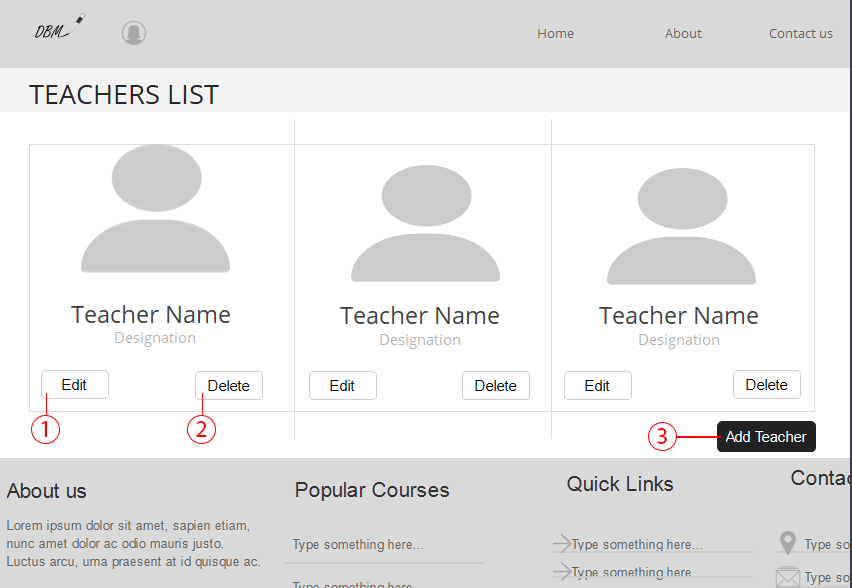
\includegraphics[width=10cm, height=11cm]{TeacherDetails(Admin)}
  \caption{Teacher Details}
\end{figure}
\begin{longtable}{|>{\raggedright\arraybackslash}p{2.5cm}|>{\raggedright\arraybackslash}p{4cm}|>{\raggedright\arraybackslash}p{2.2cm}|>{\raggedright\arraybackslash}p{2cm}|>{\raggedright\arraybackslash}p{2cm}|}
\hline
\textbf{Component} & \textbf{Description} & \textbf{Mandatory} & \textbf{Validation} & \textbf{Type}\\
\hline
% Row 1 start
1 &
To edit teachers details. &
None &
None &
None \\
% Row 1 end
\hline

% Row 2 start
2 &
Deletes teacher from the record. &
None &
None &
None \\
% Row 2 end
\hline

% Row 3 start
3 &
Add new teacher in record. &
None &
None &
None \\
% Row 3 end
\hline

\caption{Teacher details}
\end{longtable}

\newpage

%\subsubsection{Add Teacher}
%\begin{figure}[h]
%  \centering
%  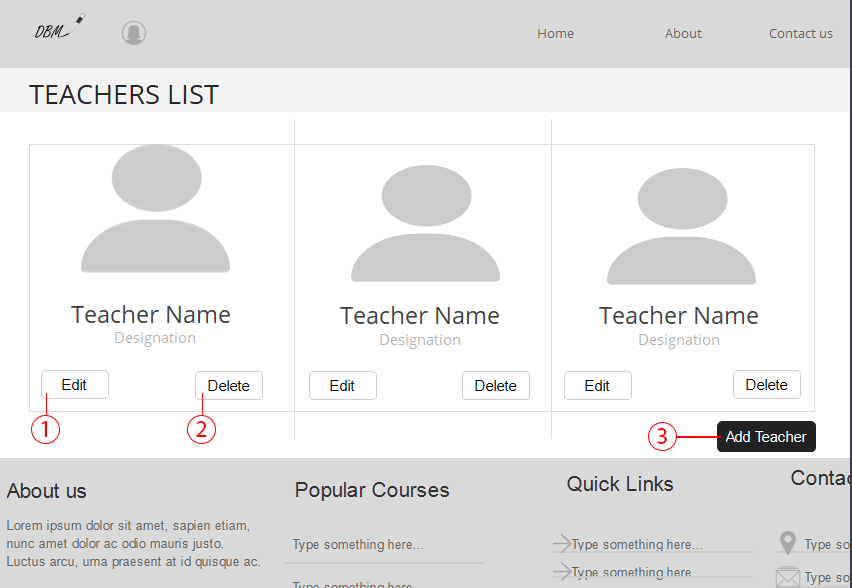
\includegraphics[width=6cm, height=6cm]{TeacherDetails(Admin)}
%  \caption{Add Teacher}
%\end{figure}



\subsubsection{Permission Management}
\begin{figure}[h]
  \centering
  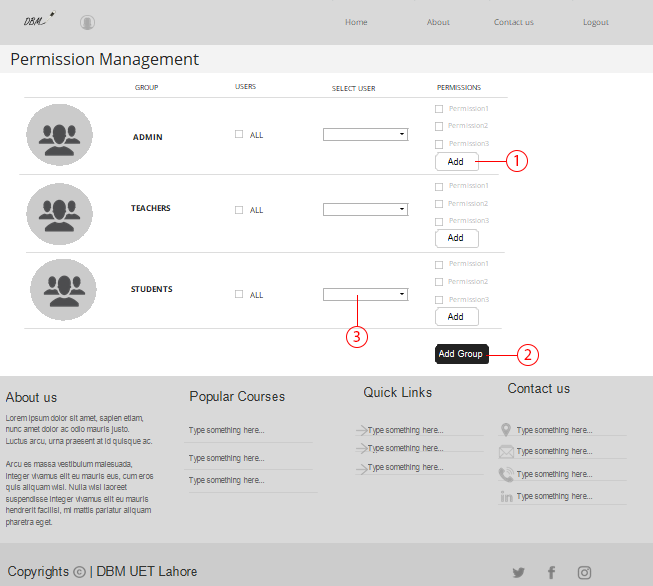
\includegraphics[width=12cm, height=12cm]{PermissionManagement(Admin)}
  \caption{Permission Management}
\end{figure}
\begin{longtable}{|>{\raggedright\arraybackslash}p{2.5cm}|>{\raggedright\arraybackslash}p{4cm}|>{\raggedright\arraybackslash}p{2.2cm}|>{\raggedright\arraybackslash}p{2cm}|>{\raggedright\arraybackslash}p{2cm}|}
\hline
\textbf{Component} & \textbf{Description} & \textbf{Mandatory} & \textbf{Validation} & \textbf{Type}\\
\hline
% Row 1 start
1 &
To add new permissions. &
None &
None &
None \\
% Row 1 end
\hline

% Row 2 start
2 &
Select user to allow for permissions. &
None &
None &
None \\
% Row 2 end
\hline

% Row 3 start
3 &
Add new group for permission. &
None &
None &
None \\
% Row 3 end
\hline

\caption{Manage Permissions}
\end{longtable}

\newpage

\subsubsection{Add Groups for Permission Management}
\begin{figure}[h]
  \centering
  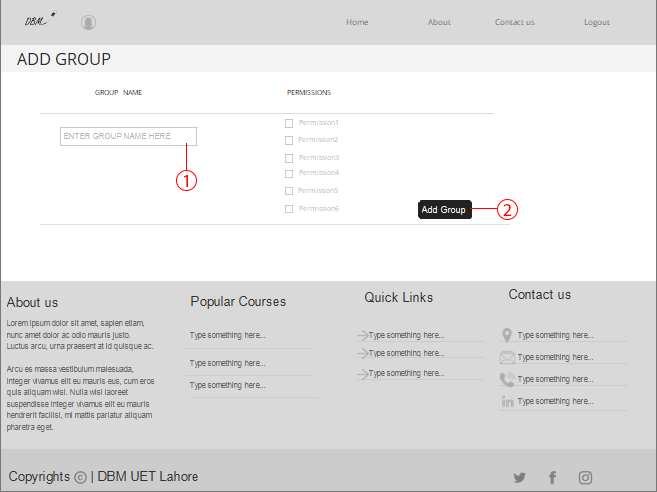
\includegraphics[width=12cm, height=13cm]{AddGroups(Admin)}
  \caption{Add Groups}
\end{figure}
\begin{longtable}{|>{\raggedright\arraybackslash}p{2.5cm}|>{\raggedright\arraybackslash}p{4cm}|>{\raggedright\arraybackslash}p{2.2cm}|>{\raggedright\arraybackslash}p{2cm}|>{\raggedright\arraybackslash}p{2cm}|}
\hline
\textbf{Component} & \textbf{Description} & \textbf{Mandatory} & \textbf{Validation} & \textbf{Type}\\
\hline
% Row 1 start
1 &
Group name. &
Yes &
None &
String \\
% Row 1 end
\hline

% Row 2 start
2 &
Save record in database. &
None &
None &
None \\
% Row 2 end
\hline

\caption{Add Groups}
\end{longtable}

\newpage

%\subsubsection{About Page}
%Everyone can see this about page. It has all our information related to DBM.
%\begin{figure}[h]
%  \centering
%  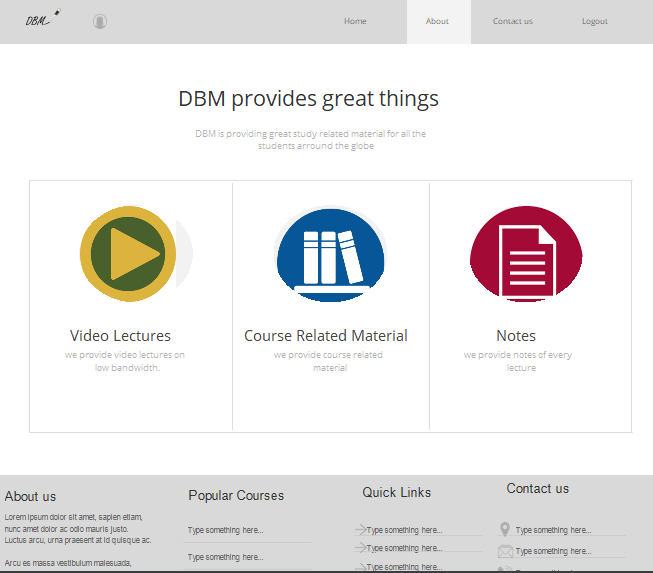
\includegraphics[width=6cm, height=6cm]{AboutPage}
%  \caption{About}
%\end{figure}
%
%\subsection{Working Flow}
%\subsubsection{Teacher}
%\begin{figure}[h]
%  \centering
%  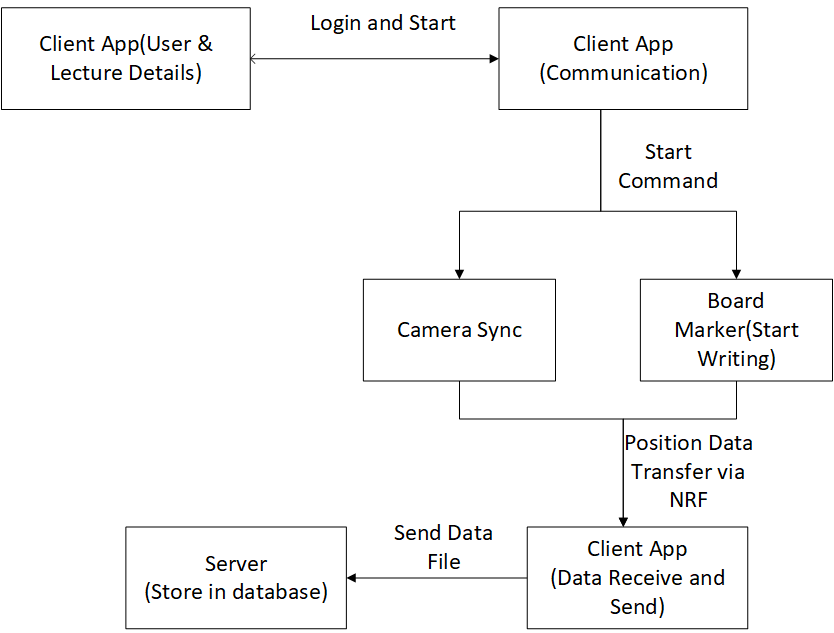
\includegraphics[width=13cm, height=13cm]{TeacherFlowDiagram}
%  \caption{Working flow for teacher}
%\end{figure}
%\newpage
%
%\subsubsection{Student}
%\begin{figure}[h]
%  \centering
%  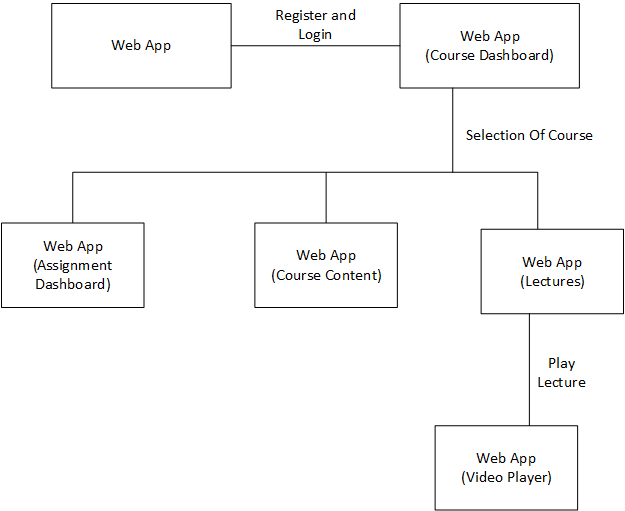
\includegraphics[width=13cm, height=13cm]{StudentFlowDiagram}
%  \caption{Working flow for Student}
%\end{figure}
%\newpage
%
%
%

\newpage
\subsection{User Interfaces (Offline Player)}
Offline player has three major sub-modules lecture playlist, token authentication, lecture player.
\subsubsection{Lecture Player}

\paragraph{Short Description}\mbox{}\\
The objective of offline player sub-module Lecture player is to downloaded lectures play offline in the application. The challenge is to move lecture video to a specific position. This application is developed in visual studio as windows form application.
\paragraph{Component Diagram}\mbox{}\\
Diagram of lecture player page is shown:
\begin{figure}[h]
\begin{center}
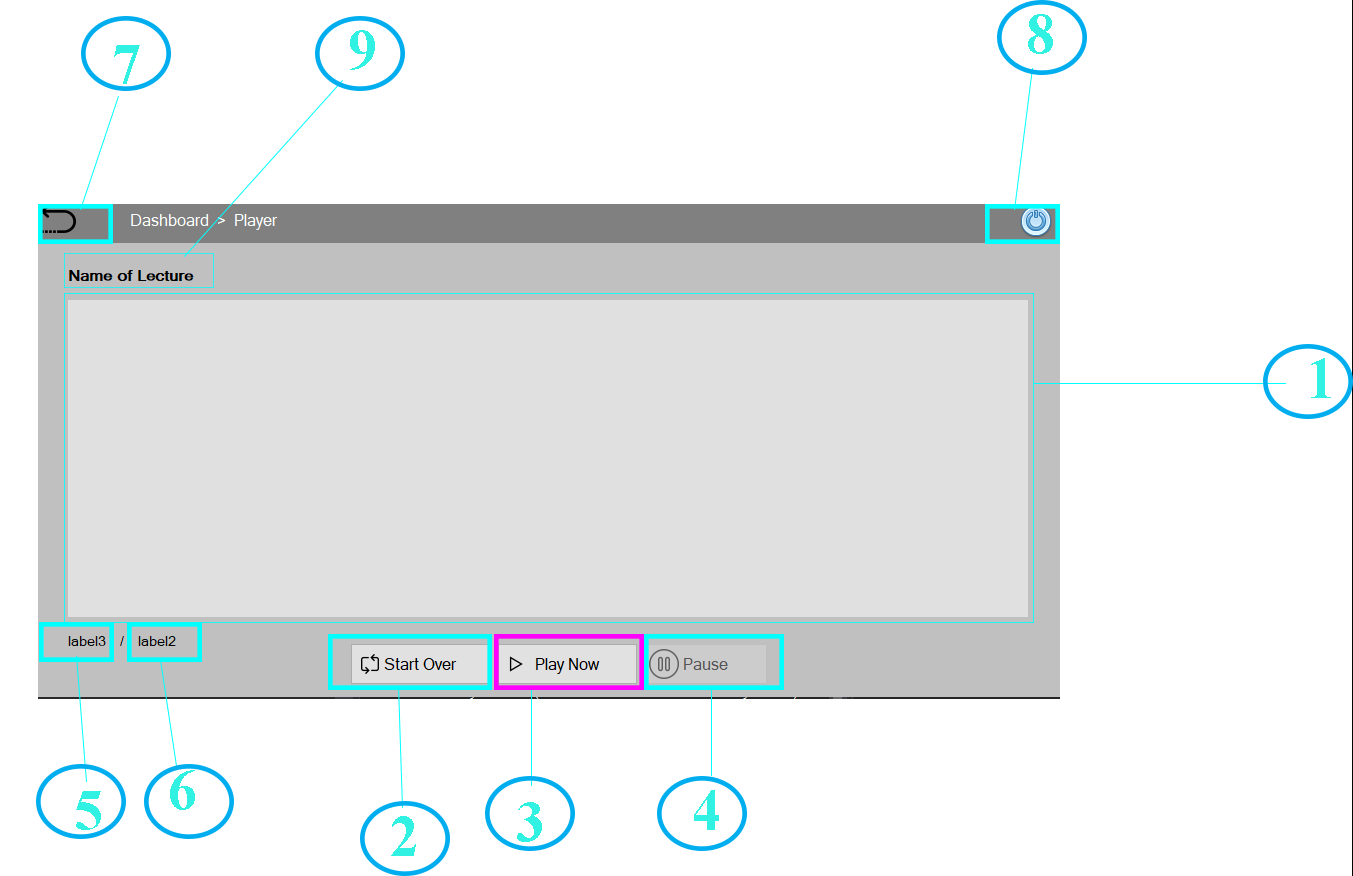
\includegraphics[width=12cm, height=8cm]{labeled_player}
\end{center}
\caption{lecture player details}
\end{figure}
\newpage

\begin{center}
 \begin{longtable}{|p{2cm}|p{7cm}|p{4cm}|} 
 \hline
 Component number & Description & Component Diagram \\ [0.5ex] 
 \hline
\hline 
1&\textbf{Name:} Player Screen\\&\textbf{Details:} Player screen is a place where animated video drawn by data in json file will be played.& \begin{minipage}{.3\textwidth}
      
\includegraphics[width=\linewidth, height=20mm]{Player_Screen}
    \end{minipage}\\
\hline
 2 &
  \textbf{Name:} Start Over Button\\&
\textbf{Details:} This button is responsible for suspending all the threads except main thread and play the video, audio and timer from the start.& \begin{minipage}{.3\textwidth}
      
\includegraphics[width=\linewidth, height=20mm]{Start_Over_Button}
    \end{minipage}\\
 \hline 3 &
  \textbf{Name:} Play Now Button\\&
\textbf{Details:} This play now button starts three new threads of audio, video and timer start it is responsible to play video at start.&\begin{minipage}{.3\textwidth}
      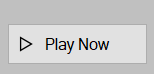
\includegraphics[width=\linewidth, height=20mm]{Play_Now_Button}
    \end{minipage}\\
 \hline 4 &
  \textbf{Name:} Pause Button\\&
\textbf{Details:} It pauses the audio, video and timer at a specific time when they have been played. It suspends all threads which are responsible to play video for a time being.& \begin{minipage}{.3\textwidth}
      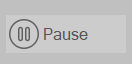
\includegraphics[width=\linewidth, height=20mm]{Pause_Button}
    \end{minipage}\\
  \hline 5 &
  \textbf{Name:} Elapsed Time Label\\&
\textbf{Details:} This label is responsible to show the elapsed time to the user so that he can keep track of video.& \begin{minipage}{.3\textwidth}
      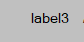
\includegraphics[width=\linewidth, height=20mm]{Elapsed_Time_Label}
    \end{minipage}\\
  \hline 6 &
  \textbf{Name:} Total Time Label\\&
\textbf{Details:}  This label shows total time of video at which it will be finished.& \begin{minipage}{.3\textwidth}
      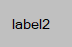
\includegraphics[width=\linewidth, height=20mm]{Total_Time_Label}
    \end{minipage}\\
  \hline 7 &
  \textbf{Name:} Go-Back Button\\&
\textbf{Details:} This button takes the user to the previous screen of lecture playlist where he or she can select any other lecture to download and play.& \begin{minipage}{.3\textwidth}
      
\includegraphics[width=\linewidth, height=20mm]{Go_Back_Button}
    \end{minipage}\\
  \hline 8 &
  \textbf{Name:} Exit Button\\&
\textbf{Details:} As it is quite obvious by the name it exits the application.& \begin{minipage}{.3\textwidth}
      
\includegraphics[width=\linewidth, height=20mm]{Exit_Button}
    \end{minipage}\\
  \hline 9 &
  \textbf{Name:} Name of Lecture Label\\&
\textbf{Details:} This label shows the name of lecture currently playing on the player selected by the user on previous screen.& \begin{minipage}{.3\textwidth}
      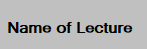
\includegraphics[width=\linewidth, height=20mm]{NameOfLectureLabel}
    \end{minipage}\\
  \hline
     
\end{longtable}
\end{center}


\subsubsection{Token based Authentication}
\paragraph{Short Description}\mbox{}\\
The objective of this sub module is to secure application. Token based authentication with web API will be done and token will be stored in local database. The challenge is we have to keep track of the token expiry on which we are providing privileges to the user. This sub module includes visual studio, and SQLite tools and windows form application technology with C\# and SQL Languages.
\newpage
\paragraph{Diagram}\mbox{}\\
Diagram of authentication page is shown:
\begin{figure}[h]
\includegraphics[width=15cm, height=13cm]{labeled_authentication}
\caption{token authentication details}
\end{figure}
\newpage
\begin{center}
 \begin{longtable}{|p{2cm}|p{9cm}|p{4cm}|} 
 \hline
 Component number & Description & Component Diagram \\ [0.5ex] 
 \hline
\hline 
1&\textbf{Name:} Username Input\\&\textbf{Details:} Username input takes valid username from user at the time of authentication& \begin{minipage}{.3\textwidth}
      \includegraphics[width=\linewidth, height=20mm]{usernameinput}
    \end{minipage}\\
\hline
 2 &
  \textbf{Name:} Password Input\\&
\textbf{Details:} password input takes a password corresponding to given username.& \begin{minipage}{.3\textwidth}
      \includegraphics[width=\linewidth, height=20mm]{passwordinput}
    \end{minipage}\\
 \hline 3 &
  \textbf{Name:} Login Button\\&
\textbf{Details:} Login button contacts with WEB API for token info for given username and password.&\begin{minipage}{.3\textwidth}
      \includegraphics[width=\linewidth, height=20mm]{loginbutton}
    \end{minipage}\\
 \hline     
\end{longtable}
\end{center}

\subsubsection{Rules and Assumption}
Following are rules and cases of assumptions that are assumed to be true while normal working.
\begin{itemize}
\item Suitable Operating System must be installed on System such windows XP and higher.
\item Suitable Version of .net framework should be installed on system otherwise we have to install app with manifest files.
\end{itemize}

\subsubsection{Module Workflow Description}
\paragraph{User General Flow}
\begin{itemize}
\item User starts the application.
\item For first time application needs authentication from user to save token information in local database.
\item Once user is authenticated, he can view lecture playlist via internet connectivity.
\item User can download and play lectures.
\end{itemize}

\paragraph{User General Flow Diagram}\mbox{}\\
\begin{figure}[h]
\includegraphics[scale=1.0]{userworkflow}
\caption{General User Workflow}
\end{figure}


\newpage
\paragraph{Application General Flow}\mbox{}\\
\begin{itemize}
\item Application at start checks in local database for user token and its expiry date if it is expired app asks for authentication again if not it proceeds.
\item Application checks for internet connectivity if found it fetches new lecture records from website if not it shows previously fetched and downloaded lectures. Here downloaded lectures can be played.
\end{itemize}

\paragraph{Application General Flow Diagram}\mbox{}\\
\begin{figure}[h]
\begin{center}
\includegraphics[width=8cm, height=10cm]{applicationworkflow}
\caption{General Application Workflow}
\end{center}
\end{figure}

\newpage
\subsection{Use Case Diagram}
\mbox\\
\mbox\\
\begin{figure}[h]
\begin{center}
\includegraphics[width=10cm, height=13cm]{DBMUseCaseWebAppPart1}
\caption{Use Case Diagram Web App(1)}
\end{center}
\end{figure}

\newpage
\mbox\\
\mbox\\
\begin{figure}[h]
\begin{center}
\includegraphics[width=10cm, height=13cm]{DBMUseCaseWebAppPart2}
\caption{Use Case Diagram Web App(2)}
\end{center}
\end{figure}


\newpage
\begin{figure}[h]
\begin{center}
\includegraphics[width=10cm, height=13cm]{PlayerApplication}
\caption{Player Application}
\end{center}
\end{figure}


\newpage
\mbox\\
\begin{figure}[h]
\begin{center}
\includegraphics[width=10cm, height=13cm]{ControllerApplication}
\caption{Controller Application}
\end{center}
\end{figure}

\newpage
\subsection{Use Cases(Web App)}
%\subsubsection{Web App}
\subsubsection{Use Case UC-1: User Registration}
\textbf{Stakeholders: } University, Educational Institutes \\
\textbf{Primary Actors: } Student, Teacher \\
\textbf{Post Condition: }\\
User data successfully sent to admin request approval page.\\
\textbf{Main Success Scenario: }
\begin{enumerate}
\item User wants to register.
\item User clicks on the Register link from the main Page header.
\item Registration page will be open by the system.
\item User will enter First Name, Last Name, Email, CNIC, Password and Date of birth.
\item User will select Institute name from the select list.
\item User select whether he is teacher or a student from the select list.
\item If user is student then system will show a input box for student registration No.
\item Student will enter his registration Number.
\item User clicks the \textbf{Sign Up} button.
\item System then send data to the Admin Request Approval page for the student request approval. 
\end{enumerate}
\textbf{Alternative Flow: }\\
\\
*a. At any time system fails.
\begin{enumerate}
\item User must check the internet connectivity.
\item Restart the browser and try again.
\item Try after sometime might be servers are down.
\end{enumerate}
3a. Registration page is not opened.
\begin{enumerate}
\item Refresh the browser.
\item Reload the page and try again.
\end{enumerate}
4a. User entered the invalid First Name, Last Name.
\begin{enumerate}
\item System will show the error message.
\item System will ask the user to enter the data again.
\end{enumerate}
4b. User entered the invalid Email.
\begin{enumerate}
\item System will show the error message.
\item System will ask the user to enter the data again.
\end{enumerate}
4c. User entered the invalid CNIC.
\begin{enumerate}
\item System will show the error message.
\item System will ask the user to enter the data again.
\end{enumerate}
4d. User entered the invalid Registration No.
\begin{enumerate}
\item System will show the error message.
\item System will ask the user to enter the data again.
\end{enumerate}
4e. User entered the invalid Date of birth.
\begin{enumerate}
\item System will show the error message.
\item System will ask the user to enter the data again.
\end{enumerate}
8a. Student entered the registration No. in invalid format.
\begin{enumerate}
\item System will show the error message.
\item System will ask the user to enter the data again.
\end{enumerate}
9a. Required fields are empty.
\begin{enumerate}
\item System will show the error message.
\item System will ask the user to complete all the required fields.
\end{enumerate}
9b. Sign Up button is not clicked.
\begin{enumerate}
\item information will be saved as a draft for later use.
\end{enumerate}
\textbf{Frequency of Occurrence:}\\
One time per user.



\subsubsection{Use Case UC-2: User Login}
\textbf{Stakeholders: } University, Educational Institutes \\
\textbf{Primary Actors: } Student, Teacher, Admin \\
\textbf{Preconditions: }
\begin{itemize}
\item User is approved by the admin.
\item User is identified and authenticated.
\item User's record is saved.
\end{itemize}
\textbf{Post Condition: }
\begin{itemize}
\item User is logged in into the system.
\item User has access to different functionality of the system.
\end{itemize}
\newpage
\textbf{Main Success Scenario:}
\begin{enumerate}
\item User wants to login.
\item User clicked on the login link to access the login page from the header.
\item System open the login page for the user.
\item User enter email address along with the password.
\item User clicked the \textbf{Sign In} button.
\item System validates the user email and password.
\item System will redirect the user to next page.
\end{enumerate}
\textbf{Alternative Flows:}\\
\\
*a. At any time, system fails.
\begin{enumerate}
\item User must check the internet connectivity.
\item Restart the browser and try again.
\item Try after sometime might be servers are down.
\end{enumerate}
3a. Login page is not opened.
\begin{enumerate}
\item Refresh the browser.
\item Reload the page and try again.
\end{enumerate}
4a. User entered invalid email and password.
\begin{enumerate}
\item System will show the error message.
\item System will ask the user to enter the data again.
\end{enumerate}
5a. Required fields are empty.
\begin{enumerate}
\item System will show the error message.
\item System will ask the user to complete all the required fields.
\end{enumerate}
6a. User is not identified or authenticated.
\begin{enumerate}
\item System will show error message.
\item System will ask the user to register yourself first.
\end{enumerate}
\textbf{Frequency of Occurrence:}\\
Whenever the user wants to login.



\subsubsection{Use Case UC-3: Forget Password}
\textbf{Stakeholders: } University, Educational Institutes \\
\textbf{Primary Actors: } Student, Teacher \\
\textbf{Precondition:}\begin{itemize}
\item User is approved by the admin.
\item User is identified and authenticated.
\item User's record is saved.
\item Login page is opened.
\end{itemize}
\textbf{Post Condition: }\\
Password reset successfully by the system.\\
\textbf{Main Success Scenario:}
\begin{enumerate}
\item User forgets his password.
\item User wants to reset his password.
\item User clicks on link \textbf{forget password}.
\item System open the \textbf{forget password} page for the user.
\item User enter CNIC, new password, confirm password.
\item User click on \textbf{Set Password} button.
\item System validate the User.
\item System resets the user password.
\end{enumerate}
\textbf{Alternative Flows:}\\\\
*a. At any time, system fails.
\begin{enumerate}
\item User must check the internet connectivity.
\item Restart the browser and try again.
\item Try after sometime might be servers are down.
\end{enumerate}
3a. Forget password page is not opened.
\begin{enumerate}
\item Refresh the browser.
\item Reload the page and try again.
\end{enumerate}
4a. User enter invalid data.
\begin{enumerate}
\item System will show the error message.
\item System will ask the user to enter the data again.
\end{enumerate}
4b. New password and confirm password don't match.
\begin{enumerate}
\item System will show the error message.
\item System will ask the user to enter the data again.
\end{enumerate}
5a. Required fields are empty.
\begin{enumerate}
\item System will show the error message.
\item System will ask the user to fill all the required fields.
\end{enumerate}
6a. User is not identified or authenticated.
\begin{enumerate}
\item System will show error message.
\item System will ask the user to register yourself first.
\end{enumerate}
\textbf{Frequency of Occurrence:}\\
Whenever the user wants to reset his password.


\subsubsection{Use Case UC-4: Teacher's Requests Approval}
\textbf{Stakeholders: } University, Educational Institutes \\
\textbf{Primary Actors: } Admin \\
\textbf{Preconditions:}
\begin{itemize}
\item Admin is logged in the system..
\item Admin is identified and authenticated.
\end{itemize}
\textbf{Post Conditions: }
\begin{itemize}
\item Requests are approved / disapproved.
\item On approval / disapproval, Email is sent to the teacher.
\item Teachers can login to the system.
\end{itemize}
\textbf{Main Success Scenario:}
\begin{enumerate}
\item Admin wants to handle the requests of teachers.
\item Admin clicks on the Teacher requests approval link from the header.
\item System open the \textbf{teachers request approval} page for the admin.
\item Admin can see the list of all the requests of teachers.
\item Admin clicks on the \textbf{Approve} button for approval of request.
\item System send the approval email to that teacher.
\item System show the success message to admin that email is sent.
\item System saves the record of the teacher.
\item System removes the request from the page.
\item Admin disapprove the request of a teacher by clicking on \textbf{Disapprove} button.
\item System delete that temporary record of the user.
\item System send an disapproval email to the teacher.
\item System show the success message to admin that email is sent.
\item System removes the request from the page.
\end{enumerate}
\textbf{Alternative Flows:}\\
\\
*a. At any time, system fails.
\begin{enumerate}
\item User must check the internet connectivity.
\item Restart the browser and try again.
\item Try after sometime might be servers are down.
\end{enumerate}
3a. Page is not opened.
\begin{enumerate}
\item Refresh the browser.
\item Reload the page and try again.
\end{enumerate}
5a. Approve button is not working properly.
\begin{enumerate}
\item Admin must have to refresh the page.
\item Restart the browser and try again.
\item May be some backend issue, resolve that issue.
\end{enumerate}
6-7a. Email is not sent to the teacher.
\begin{enumerate}
\item Admin must again approve the request of teacher.
\item May be some backend issue, resolve that issue.
\end{enumerate}
8-9a. Request is not removed from the page and record is unsaved.
\begin{enumerate}
\item Admin must again approve the request of teacher.
\item May be some backend issue, resolve that issue.
\end{enumerate}
10a. Disapprove button is not working properly.
\begin{enumerate}
\item Admin must have to refresh the page.
\item Restart the browser and try again.
\item May be some backend issue, resolve that issue.
\end{enumerate}
12-13a. Email is not sent to the teacher.
\begin{enumerate}
\item Admin must again approve the request of teacher.
\item May be some backend issue, resolve that issue.
\end{enumerate}
14a. Request is not removed from the page.
\begin{enumerate}
\item Admin must again approve the request of teacher.
\item May be some backend issue, resolve that issue.
\end{enumerate}
\textbf{Frequency of Occurrence:}\\
Whenever the requests appear on the page.
\\
\textbf{Open Issues:}\\
What will happen if admin has mistakenly approve or disapprove the request of teacher?


\subsubsection{Use Case UC-5: Student's Requests Approval}
\textbf{Stakeholders: } University, Educational Institutes \\
\textbf{Primary Actors: } Admin \\
\textbf{Preconditions:}
\begin{itemize}
\item Admin is logged in the system..
\item Admin is identified and authenticated.
\end{itemize}
\textbf{Post Conditions: }
\begin{itemize}
\item Requests are approved / disapproved.
\item On approval / disapproval, Email is sent to the student.
\item Students can login to the system.
\end{itemize}
\textbf{Main Success Scenario:}
\begin{enumerate}
\item Admin wants to handle the requests of students.
\item Admin clicks on the student requests approval link from the header.
\item System open the \textbf{Students Request Approval} page for the admin.
\item Admin can see the list of all the request of students.
\item Admin clicks on the \textbf{Approve} button for approval of request.
\item System send the approval email to that student.
\item System show the success message to admin that email is sent.
\item System saves the record of the student.
\item System removes the request from the page.
\item Admin disapprove the request of a student by clicking on \textbf{disapprove} button.
\item System delete that temporary record of the user.
\item System send an disapproval email to the student.
\item System show the success message to admin that email is sent.
\item System removes the request from the page.
\end{enumerate}
\textbf{Alternative Flows:}\\
\\
*a. At any time, system fails.
\begin{enumerate}
\item User must check the internet connectivity.
\item Restart the browser and try again.
\item Try after sometime might be servers are down.
\end{enumerate}
3a. Page is not opened.
\begin{enumerate}
\item Refresh the browser.
\item Reload the page and try again.
\end{enumerate}
5a. Approve button is not working properly.
\begin{enumerate}
\item Admin must have to refresh the page.
\item Restart the browser and try again.
\item May be some backend issue, resolve that issue.
\end{enumerate}
6-7a. Email is not sent to the student.
\begin{enumerate}
\item Admin must again approve the request of student.
\item May be some backend issue, resolve that issue.
\end{enumerate}
8-9a. Request is not removed from the page and record is unsaved.
\begin{enumerate}
\item Admin must again approve the request of student.
\item May be some backend issue, resolve that issue.
\end{enumerate}
10a. Disapprove button is not working properly.
\begin{enumerate}
\item Admin must have to refresh the page.
\item Restart the browser and try again.
\item May be some backend issue, resolve that issue.
\end{enumerate}
12-13a. Email is not sent to the teacher.
\begin{enumerate}
\item Admin must again approve the request of student.
\item May be some backend issue, resolve that issue.
\end{enumerate}
14a. Request is not removed from the page.
\begin{enumerate}
\item Admin must again approve the request of student.
\item May be some backend issue, resolve that issue.
\end{enumerate}
\textbf{Frequency of Occurrence:}\\
Whenever the admin get requests from students.
\\
\textbf{Open Issues:}\\
What will happen if admin has mistakenly approve or disapprove the request of student?


\subsubsection{Use Case UC-6: Add New Course}
\textbf{Stakeholders: } University, Educational Institutes \\
\textbf{Primary Actors: } Admin \\
\textbf{Preconditions:}
\begin{itemize}
\item Admin is logged in the system.
\item Admin is identified and authenticated.
\end{itemize}
\textbf{Post Condition: }\\
Course is added successfully.\\
\textbf{Main Success Scenario:}
\begin{enumerate}
\item Admin want to add new course.
\item He clicks on the course link from the header.
\item All courses screen will be open.
\item Admin clicks the \textbf{Add Course} button to add new course.
\item System open a new page.
\item Admin add all course related information.
\item Admin clicks the \textbf{Submit} button. 
\end{enumerate}
\textbf{Alternative Flows:}\\
*a. At any time, System fails.
\begin{enumerate}
\item User must check the internet connectivity.
\item Restart the browser and try again.
\item Try after sometime might be servers are down.
\end{enumerate}
2a. Courses link is not shown on the header.
\begin{enumerate}
\item Admin must have to refresh the page.
\item Restart the browser and try again.
\end{enumerate} 
3a. All courses page is not opened.
\begin{enumerate}
\item Admin must check the internet connectivity.
\item Refresh the browser.
\item Reload the page and try again.
\end{enumerate}
4a. Add button not working.
\begin{enumerate}
\item Admin must check the internet connectivity.
\item Refresh the browser.
\item Reload the page and try again.
\item May be some backend issue, try to resolve that issue.
\end{enumerate}
5a. New page is not appearing.
\begin{enumerate}
\item Admin must check the internet connectivity.
\item Refresh the browser.
\item Try for sometime, may be servers are down.
\end{enumerate}
6a. Admin enter invalid data.
\begin{enumerate}
\item System will prompt an error message.
\item System will ask the user to enter valid data.
\end{enumerate}
7a. Required fields are empty.
\begin{enumerate}
\item System will prompt an error message.
\item System will ask the user to enter all the required information.
\end{enumerate}
7b. Admin don't click on \textbf{Add} button.
\begin{enumerate}
\item System will save the record as draft for later use.
\end{enumerate}
\textbf{Frequency of Occurrence:}\\
Whenever the admin wants to add new course.



\subsubsection{Use Case UC-7: Edit Course}
\textbf{Stakeholders: } University, Educational Institutes \\
\textbf{Primary Actors: } Admin \\
\textbf{Preconditions:}
\begin{itemize}
\item Admin is logged in the system.
\item Admin is identified and authenticated.
\item Course must be added.
\end{itemize}
\textbf{Post Condition: }\\
Course is updated successfully.\\
\newpage
\textbf{Main Success Scenario:}
\begin{enumerate}
\item Admin wants to edit particular course.
\item Admin clicks on the courses link from the header.
\item System open a page of all courses.
\item Admin click on the \textbf{Edit} button of course which he wants to update.
\item Course Edit screen will appear.
\item Admin update the required information.
\item Admin clicks the \textbf{Update Course} button.
\item System update the course.
\end{enumerate}
\textbf{Alternative Flows:}\\
\\
*a. At any time, System fails.
\begin{enumerate}
\item User must check the internet connectivity.
\item Restart the browser and try again.
\item Try after sometime might be servers are down.
\end{enumerate}
2a. Courses link is not shown on the header.
\begin{enumerate}
\item Admin must have to refresh the page.
\item Restart the browser and try again.
\end{enumerate} 
3a. All courses page is not opened.
\begin{enumerate}
\item Admin must check the internet connectivity.
\item Refresh the browser.
\item Reload the page and try again.
\end{enumerate}
4a. Edit button not working.
\begin{enumerate}
\item Admin must check the internet connectivity.
\item Refresh the browser.
\item Reload the page and try again.
\item May be some backend issue, try to resolve that issue.
\end{enumerate}
5a. Edit Course page is not appearing.
\begin{enumerate}
\item Admin must check the internet connectivity.
\item Refresh the browser.
\item Try for sometime, may be servers are down.
\end{enumerate}
6a. Admin enter invalid data.
\begin{enumerate}
\item System will prompt an error message.
\item System will ask the user to enter valid data.
\end{enumerate}
7a. Required fields are empty.
\begin{enumerate}
\item System will prompt an error message.
\item System will ask the user to enter all the required information.
\end{enumerate}
7b. Admin don't click on \textbf{Update Course} button.
\begin{enumerate}
\item System will save the record as draft for later use.
\end{enumerate}
\textbf{Frequency of Occurrence:}\\
Whenever the user wants to update the course information.



\subsubsection{Use Case UC-8: Delete Course}
\textbf{Stakeholders: } University, Educational Institutes \\
\textbf{Primary Actors: } Admin \\
\textbf{Preconditions:}
\begin{itemize}
\item Admin is logged in the system.
\item Admin is identified and authenticated.
\item Course must be added.
\end{itemize}
\textbf{Post Condition: }\\
Course is deleted successfully.\\
\textbf{Main Success Scenario:}
\begin{enumerate}
\item Admin wants to delete particular course.
\item Admin clicks on the courses link from the header.
\item System open a page of all courses.
\item Admin click on the \textbf{Delete} button of course which he wants to delete.
\item A pop message show "Are you sure you want to delete the course?".
\item Admin clicks the sure button.
\item System delete that course from the record.
\end{enumerate}
\textbf{Alternative Flows:}\\
\\
*a. At any time, System fails.
\begin{enumerate}
\item User must check the internet connectivity.
\item Restart the browser and try again.
\item Try after sometime might be servers are down.
\end{enumerate}
2a. Courses link is not shown on the header.
\begin{enumerate}
\item Admin must have to refresh the page.
\item Restart the browser and try again.
\end{enumerate} 
3a. All courses page is not opened.
\begin{enumerate}
\item Admin must check the internet connectivity.
\item Refresh the browser.
\item Reload the page and try again.
\end{enumerate}
4a. Delete button not working.
\begin{enumerate}
\item Admin must check the internet connectivity.
\item Refresh the browser.
\item Reload the page and try again.
\item May be some backend issue, try to resolve that issue.
\end{enumerate}
5a. Admin clicks the sure button but course is not deleted.
\begin{enumerate}
\item May be servers are down. Try again after sometime.
\item Press again the delete button.
\end{enumerate}
\textbf{Frequency of Occurrence:}\\
Whenever the admin wants to delete a course.
\textbf{Open Issues:}\\
What will happen if admin has mistakenly deleted the course?



\subsubsection{Use Case UC-9: View Courses}
\textbf{Stakeholders: } University, Educational Institutes \\
\textbf{Primary Actors: }Admin,Teacher, Student \\
\textbf{Preconditions:}
\begin{itemize}
\item User is logged in the system.
\item User is identified and authenticated.
\item Courses must be added.
\end{itemize}
\textbf{Post Condition: }\\
Courses List is viewed successfully.\\
\textbf{Main Success Scenario:}
\begin{enumerate}
\item Admin wants to view all courses.
\item Admin clicks on the courses link from the header.
\item System open a page of all courses.
\end{enumerate}
\textbf{Alternative Flows:}\\
\\
*a. At any time, System fails.
\begin{enumerate}
\item User must check the internet connectivity.
\item Restart the browser and try again.
\item Try after sometime might be servers are down.
\end{enumerate}
2a. Courses link is not shown on the header.
\begin{enumerate}
\item Admin must have to refresh the page.
\item Restart the browser and try again.
\end{enumerate} 
3a. All courses page is not opened.
\begin{enumerate}
\item Admin must check the internet connectivity.
\item Refresh the browser.
\item Reload the page and try again.
\end{enumerate}
\textbf{Frequency of Occurrence:}\\
Whenever the user wants to view all course.




\subsubsection{Use Case UC-10: Upload Course Assignment}
\textbf{Stakeholders: } University, Educational Institutes \\
\textbf{Primary Actors: }Teacher \\
\textbf{Preconditions:}
\begin{itemize}
\item Teacher is logged in the system.
\item User is identified and authenticated.
\item Course is assigned to the teacher.
\end{itemize}
\textbf{Post Condition: }\\
Course assignment is uploaded successfully.\\
\textbf{Main Success Scenario:}
\begin{enumerate}
\item Teacher wants to upload course assignment.
\item Teacher clicks on the courses link from the header.
\item System opens a page of all courses.
\item Teacher clicks on the \textbf{View} button of course of which he wants to upload assignment.
\item System opens a course dashboard page.
\item Teacher clicks on the \textbf{Assignments} tab.
\item System opens the assignments page.
\item Teacher click on \textbf{Upload Assignment} button.
\item System opens upload assignment page.
\item Teacher enters all the data.
\item System validates the data.
\item Teacher press the \textbf{Upload Assignment} button.
\item System saves the assignment record.
\end{enumerate}
\textbf{Alternative Flows:}\\
\\
*a. At any time, System fails.
\begin{enumerate}
\item User must check the internet connectivity.
\item Restart the browser and try again.
\item Try after sometime might be servers are down.
\end{enumerate}
2a. Courses link is not shown on the header.
\begin{enumerate}
\item User must have to refresh the page.
\item Restart the browser and try again.
\end{enumerate} 
3a. All courses page is not opened.
\begin{enumerate}
\item User must check the internet connectivity.
\item Refresh the browser.
\item Reload the page and try again.
\end{enumerate}
4a. View button not working.
\begin{enumerate}
\item User must check the internet connectivity.
\item Refresh the browser.
\item Reload the page and try again.
\item May be some backend issue, try to resolve that issue.
\end{enumerate}
5a. Course dasboard page is not opened.
\begin{enumerate}
\item User must check the internet connectivity.
\item Refresh the browser.
\item Reload the page and try again.
\end{enumerate}
6a. Assignments tab not working.
\begin{enumerate}
\item Reload the page and try again.
\item May be some backend issue, try to resolve that issue.
\end{enumerate}
7a. Assignments page is not opened.
\begin{enumerate}
\item User must check the internet connectivity.
\item Refresh the browser.
\item Reload the page and try again.
\end{enumerate}
8a. Upload assignment button not working.
\begin{enumerate}
\item Reload the page and try again.
\item Check the internet connectivity.
\item May be some backend issue, try to resolve that issue.
\end{enumerate}
9a. Upload assignment page is not opened.
\begin{enumerate}
\item User must check the internet connectivity.
\item Refresh the browser.
\item Reload the page and try again.
\end{enumerate}
10-11a. User enter invalid data.
\begin{enumerate}
\item System will show error message.
\item System will ask the user to enter the data again.
\end{enumerate}
12a. Required fields are empty.
\begin{enumerate}
\item System will show error message.
\item System will ask the user to enter the required data. 
\end{enumerate}
\textbf{Frequency of Occurrence:}\\
Whenever user wants to upload assignments.



\subsubsection{Use Case UC-11: View Course Assignments}
\textbf{Stakeholders: } University, Educational Institutes \\
\textbf{Primary Actors: }Teacher, Student \\
\textbf{Preconditions:}
\begin{itemize}
\item User is identified and authenticated.
\item User is logged in the system.
\item Student is enrolled in that course.
\item Course is assigned to teacher.
\end{itemize}
\textbf{Post Condition: }\\
Course Assignment viewed successfully.\\
\textbf{Main Success Scenario:}
\begin{enumerate}
\item User wants to view course assignment.
\item User clicks on the courses link from the header.
\item System opens a page of all courses.
\item User clicks on the \textbf{View} button of course of which he wants to view assignment.
\item System opens a course dashboard page.
\item User clicks on the \textbf{Assignments} tab.
\item System opens the assignments page.
\end{enumerate}
\textbf{Alternative Flows:}\\
\\
*a. At any time, System fails.
\begin{enumerate}
\item User must check the internet connectivity.
\item Restart the browser and try again.
\item Try after sometime might be servers are down.
\end{enumerate}
2a. Courses link is not shown on the header.
\begin{enumerate}
\item User must have to refresh the page.
\item Restart the browser and try again.
\end{enumerate} 
3a. All courses page is not opened.
\begin{enumerate}
\item User must check the internet connectivity.
\item Refresh the browser.
\item Reload the page and try again.
\end{enumerate}
4a. View button not working.
\begin{enumerate}
\item User must check the internet connectivity.
\item Refresh the browser.
\item Reload the page and try again.
\item May be some backend issue, try to resolve that issue.
\end{enumerate}
5a. Course dasboard page is not opened.
\begin{enumerate}
\item User must check the internet connectivity.
\item Refresh the browser.
\item Reload the page and try again.
\end{enumerate}
6a. Assignments tab not working.
\begin{enumerate}
\item Reload the page and try again.
\item May be some backend issue, try to resolve that issue.
\end{enumerate}
7a. Assignments page is not opened.
\begin{enumerate}
\item User must check the internet connectivity.
\item Refresh the browser.
\item Reload the page and try again.
\end{enumerate}
\textbf{Frequency of Occurrence:}\\
Whenever user wants to view assignments.



\subsubsection{Use Case UC-12: Download Course Assignment}
\textbf{Stakeholders: } University, Educational Institutes \\
\textbf{Primary Actors: }Teacher, Student \\
\textbf{Preconditions:}
\begin{itemize}
\item User is logged in the system.
\item User is identified and authenticated.
\item Course is assigned to the teacher.
\item Student is enrolled in that course.
\end{itemize}
\textbf{Post Condition: }\\
Course assignment is downloaded successfully.\\
\textbf{Main Success Scenario:}
\begin{enumerate}
\item User wants to download course assignment.
\item User clicks on the courses link from the header.
\item System opens a page of all courses.
\item User clicks on the \textbf{View} button of course of which he wants to download assignment.
\item System opens a course dashboard page.
\item User clicks on the \textbf{Assignments} tab.
\item System opens the assignments page.
\item User click on \textbf{Download Assignment} button.
\item System downloads the assignment file for the user.
\end{enumerate}
\textbf{Alternative Flows:}\\
\\
*a. At any time, System fails.
\begin{enumerate}
\item User must check the internet connectivity.
\item Restart the browser and try again.
\item Try after sometime might be servers are down.
\end{enumerate}
2a. Courses link is not shown on the header.
\begin{enumerate}
\item User must have to refresh the page.
\item Restart the browser and try again.
\end{enumerate} 
3a. All courses page is not opened.
\begin{enumerate}
\item User must check the internet connectivity.
\item Refresh the browser.
\item Reload the page and try again.
\end{enumerate}
4a. View button not working.
\begin{enumerate}
\item User must check the internet connectivity.
\item Refresh the browser.
\item Reload the page and try again.
\item May be some backend issue, try to resolve that issue.
\end{enumerate}
5a. Course dasboard page is not opened.
\begin{enumerate}
\item User must check the internet connectivity.
\item Refresh the browser.
\item Reload the page and try again.
\end{enumerate}
6a. Assignments tab not working.
\begin{enumerate}
\item Reload the page and try again.
\item May be some backend issue, try to resolve that issue.
\end{enumerate}
7a. Assignments page is not opened.
\begin{enumerate}
\item User must check the internet connectivity.
\item Refresh the browser.
\item Reload the page and try again.
\end{enumerate}
8a. Download assignment button not working.
\begin{enumerate}
\item Reload the page and try again.
\item Check the internet connectivity.
\item May be some backend issue, try to resolve that issue.
\end{enumerate}
\textbf{Frequency of Occurrence:}\\
Whenever user wants to download assignments.



\subsubsection{Use Case UC-13: Delete Course Assignment}
\textbf{Stakeholders: } University, Educational Institutes \\
\textbf{Primary Actors: }Teacher \\
\textbf{Preconditions:}
\begin{itemize}
\item Teacher is logged in the system.
\item User is identified and authenticated.
\item Course is assigned to the teacher.
\end{itemize}
\textbf{Post Condition: }\\
Course assignment is deleted successfully.\\
\textbf{Main Success Scenario:}
\begin{enumerate}
\item Teacher wants to delete course assignment.
\item Teacher clicks on the courses link from the header.
\item System opens a page of all courses.
\item Teacher clicks on the \textbf{View} button of course of which he wants to upload assignment.
\item System opens a course dashboard page.
\item Teacher clicks on the \textbf{Assignments} tab.
\item System opens the assignments page.
\item Teacher click on \textbf{Delete Assignment} button.
\item A pop message show "Are you sure you want to delete the assignment?".
\item Teacher clicks the sure button.
\item System delete that assignment from the record.
\end{enumerate}
\textbf{Alternative Flows:}\\
\\
*a. At any time, System fails.
\begin{enumerate}
\item User must check the internet connectivity.
\item Restart the browser and try again.
\item Try after sometime might be servers are down.
\end{enumerate}
2a. Courses link is not shown on the header.
\begin{enumerate}
\item User must have to refresh the page.
\item Restart the browser and try again.
\end{enumerate} 
3a. All courses page is not opened.
\begin{enumerate}
\item User must check the internet connectivity.
\item Refresh the browser.
\item Reload the page and try again.
\end{enumerate}
4a. View button not working.
\begin{enumerate}
\item User must check the internet connectivity.
\item Refresh the browser.
\item Reload the page and try again.
\item May be some backend issue, try to resolve that issue.
\end{enumerate}
5a. Course dasboard page is not opened.
\begin{enumerate}
\item User must check the internet connectivity.
\item Refresh the browser.
\item Reload the page and try again.
\end{enumerate}
6a. Assignments tab not working.
\begin{enumerate}
\item Reload the page and try again.
\item May be some backend issue, try to resolve that issue.
\end{enumerate}
7a. Assignments page is not opened.
\begin{enumerate}
\item User must check the internet connectivity.
\item Refresh the browser.
\item Reload the page and try again.
\end{enumerate}
8a. Delete assignment button not working.
\begin{enumerate}
\item Reload the page and try again.
\item May be some backend issue, try to resolve that issue.
\end{enumerate}
10-11a. Teacher clicks the sure button but assignment is not deleted.
\begin{enumerate}
\item May be servers are down. Try again after sometime.
\item Press again the delete button.
\end{enumerate}
\textbf{Frequency of Occurrence:}\\
Whenever user wants to delete assignment.



\subsubsection{Use Case UC-14: Add Course Announcement}
\textbf{Stakeholders: } University, Educational Institutes \\
\textbf{Primary Actors: }Teacher \\
\textbf{Preconditions:}
\begin{itemize}
\item Teacher is logged in the system.
\item Teacher is identified and authenticated.
\item Course is assigned to the teacher.
\end{itemize}
\textbf{Post Condition: }\\
Course Announcement is added successfully.\\
\\
\textbf{Main Success Scenario:}
\begin{enumerate}
\item Teacher wants to add course related announcement.
\item Teacher clicks on the courses link from the header.
\item System opens a page of all courses.
\item Teacher clicks on the \textbf{View} button of course of which he wants to add announcement.
\item System opens a course dashboard page.
\item Teacher clicks on the \textbf{Announcement} tab.
\item System opens the announcement page.
\item Teacher click on \textbf{Add Announcement} button.
\item System opens add announcement page.
\item Teacher enters all the data.
\item System validates the data.
\item Teacher press the \textbf{Add Announcement} button.
\item System saves the announcement record.
\end{enumerate}
\textbf{Alternative Flows:}\\
\\
*a. At any time, System fails.
\begin{enumerate}
\item User must check the internet connectivity.
\item Restart the browser and try again.
\item Try after sometime might be servers are down.
\end{enumerate}
2a. Courses link is not shown on the header.
\begin{enumerate}
\item User must have to refresh the page.
\item Restart the browser and try again.
\end{enumerate} 
3a. All courses page is not opened.
\begin{enumerate}
\item User must check the internet connectivity.
\item Refresh the browser.
\item Reload the page and try again.
\end{enumerate}
4a. View button not working.
\begin{enumerate}
\item User must check the internet connectivity.
\item Refresh the browser.
\item Reload the page and try again.
\item May be some backend issue, try to resolve that issue.
\end{enumerate}
5a. Course dasboard page is not opened.
\begin{enumerate}
\item User must check the internet connectivity.
\item Refresh the browser.
\item Reload the page and try again.
\end{enumerate}
6a. Announcement tab not working.
\begin{enumerate}
\item Reload the page and try again.
\item May be some backend issue, try to resolve that issue.
\end{enumerate}
\newpage
7a. Announcement page is not opened.
\begin{enumerate}
\item User must check the internet connectivity.
\item Refresh the browser.
\item Reload the page and try again.
\end{enumerate}
8a. Add announcement button not working.
\begin{enumerate}
\item Reload the page and try again.
\item May be some backend issue, try to resolve that issue.
\end{enumerate}
9a. Add announcement page is not opened.
\begin{enumerate}
\item User must check the internet connectivity.
\item Refresh the browser.
\item Reload the page and try again.
\end{enumerate}
\textbf{Frequency of Occurrence:}\\
Whenever user wants to add announcement.



\subsubsection{Use Case UC-15 :Edit Course Announcement}
\textbf{Stakeholders: } University, Educational Institutes \\
\textbf{Primary Actors: }Teacher \\
\textbf{Preconditions:}
\begin{itemize}
\item Teacher is identified and authenticated.
\item Teacher is logged in the system.
\item Course is assigned to the teacher.
\end{itemize}
\textbf{Post Condition: }\\
Course Announcement is updated successfully.\\
\newpage
\textbf{Main Success Scenario:}
\begin{enumerate}
\item Teacher wants to edit course related announcement.
\item Teacher clicks on the courses link from the header.
\item System opens a page of all courses.
\item Teacher clicks on the \textbf{View} button of course of which he wants to edit announcement.
\item System opens a course dashboard page.
\item Teacher clicks on the \textbf{Announcement} tab.
\item System opens the announcement page.
\item Teacher click on \textbf{Edit Announcement} button of the announcement.
\item System opens edit announcement page.
\item Teacher edit the required data.
\item System validates the data.
\item Teacher press the \textbf{Update Announcement} button.
\item System updates the announcement record.
\end{enumerate}
\textbf{Alternative Flows:}\\
\\
*a. At any time, System fails.
\begin{enumerate}
\item User must check the internet connectivity.
\item Restart the browser and try again.
\item Try after sometime might be servers are down.
\end{enumerate}
2a. Courses link is not shown on the header.
\begin{enumerate}
\item User must have to refresh the page.
\item Restart the browser and try again.
\end{enumerate} 
3a. All courses page is not opened.
\begin{enumerate}
\item User must check the internet connectivity.
\item Refresh the browser.
\item Reload the page and try again.
\end{enumerate}
4a. View button not working.
\begin{enumerate}
\item User must check the internet connectivity.
\item Refresh the browser.
\item Reload the page and try again.
\item May be some backend issue, try to resolve that issue.
\end{enumerate}
5a. Course dasboard page is not opened.
\begin{enumerate}
\item User must check the internet connectivity.
\item Refresh the browser.
\item Reload the page and try again.
\end{enumerate}
6a. Announcement tab not working.
\begin{enumerate}
\item Reload the page and try again.
\item May be some backend issue, try to resolve that issue.
\end{enumerate}
7a. Announcement page is not opened.
\begin{enumerate}
\item User must check the internet connectivity.
\item Refresh the browser.
\item Reload the page and try again.
\end{enumerate}
8a. Edit announcement button not working.
\begin{enumerate}
\item Reload the page and try again.
\item May be some backend issue, try to resolve that issue.
\end{enumerate}
9a. Update announcement page is not opened.
\begin{enumerate}
\item User must check the internet connectivity.
\item Refresh the browser.
\item Reload the page and try again.
\end{enumerate}
10a. Teacher enters the invalid data.
\begin{enumerate}
\item System prompts the error message.
\item System will ask the user to enter the data again.
\end{enumerate}
12a. Required fields are empty.
\begin{enumerate}
\item System prompts the error message.
\item System will ask the user to enter the data in the empty fields.
\end{enumerate}
\textbf{Frequency of Occurrence:}\\
Whenever user wants to update announcement.



\subsubsection{Use Case UC-16: Delete Course Announcement}
\textbf{Stakeholders: } University, Educational Institutes \\
\textbf{Primary Actors: }Teacher \\
\textbf{Preconditions:}
\begin{itemize}
\item User is identified and authenticated.
\item User is logged in the system.
\item Course is assigned to the teacher.
\end{itemize}
\textbf{Post Condition: }\\
Course announcement is deleted successfully.\\
\textbf{Main Success Scenario:}
\begin{enumerate}
\item Teacher wants to delete course announcement.
\item Teacher clicks on the courses link from the header.
\item System opens a page of all courses.
\item Teacher clicks on the \textbf{View} button of course of which he wants to delete announcement.
\item System opens a course dashboard page.
\item Teacher clicks on the \textbf{Announcements} tab.
\item System opens the announcements page.
\item Teacher click on \textbf{Delete Announcement} button.
\item A pop message show "Are you sure you want to delete the announcement?".
\item Teacher clicks the sure button.
\item System delete that announcement from the record.
\end{enumerate}
\textbf{Alternative Flows:}\\
\\
*a. At any time, System fails.
\begin{enumerate}
\item User must check the internet connectivity.
\item Restart the browser and try again.
\item Try after sometime might be servers are down.
\end{enumerate}
\newpage
2a. Courses link is not shown on the header.
\begin{enumerate}
\item User must have to refresh the page.
\item Restart the browser and try again.
\end{enumerate} 
3a. All courses page is not opened.
\begin{enumerate}
\item User must check the internet connectivity.
\item Refresh the browser.
\item Reload the page and try again.
\end{enumerate}
4a. View button not working.
\begin{enumerate}
\item User must check the internet connectivity.
\item Refresh the browser.
\item Reload the page and try again.
\item May be some backend issue, try to resolve that issue.
\end{enumerate}
5a. Course dasboard page is not opened.
\begin{enumerate}
\item User must check the internet connectivity.
\item Refresh the browser.
\item Reload the page and try again.
\end{enumerate}
6a. Announcement tab not working.
\begin{enumerate}
\item Reload the page and try again.
\item May be some backend issue, try to resolve that issue.
\end{enumerate}
\newpage
7a. Announcement page is not opened.
\begin{enumerate}
\item User must check the internet connectivity.
\item Refresh the browser.
\item Reload the page and try again.
\end{enumerate}
8a. Delete announcement button not working.
\begin{enumerate}
\item Reload the page and try again.
\item May be some backend issue, try to resolve that issue.
\end{enumerate}
10-11a. Teacher clicks the sure button but announcement is not deleted.
\begin{enumerate}
\item May be servers are down. Try again after sometime.
\item Press again the delete button.
\end{enumerate}
\textbf{Frequency of Occurrence:}\\
Whenever user wants to delete announcement.\\
\textbf{Open Issues:}\\
What will happen if teacher have mistakenly delete the announcement?



\subsubsection{Use Case UC-17: Student Assignment Submission}
\textbf{Stakeholders: } University, Educational Institutes \\
\textbf{Primary Actors: }Student \\
\textbf{Preconditions:}
\begin{itemize}
\item User is identified and authenticated.
\item User is logged in the system.
\item Student is enrolled in that course.
\end{itemize}
\textbf{Post Condition: }\\
Assignment is submitted successfully.\\
\\
\textbf{Main Success Scenario:}
\begin{enumerate}
\item Student wants to submit course assignment.
\item Student clicks on the courses link from the header.
\item System opens a page of all courses.
\item Student clicks on the \textbf{View} button of course of which he wants to submit assignment.
\item System opens a course dashboard page.
\item Student clicks on the \textbf{Assignment} tab.
\item System opens the assignment page.
\item Student click on \textbf{Submit Assignment} button.
\item System open a new page.
\item Student upload assignment file which he/she wants to submit.
\item Student clicks on the \textbf{Submit} button.
\item System save the assignment of student in the record.
\end{enumerate}
\textbf{Alternative Flows:}\\
\\
*a. At any time, System fails.
\begin{enumerate}
\item User must check the internet connectivity.
\item Restart the browser and try again.
\item Try after sometime might be servers are down.
\end{enumerate}
\newpage
2a. Courses link is not shown on the header.
\begin{enumerate}
\item User must have to refresh the page.
\item Restart the browser and try again.
\end{enumerate} 
3a. All courses page is not opened.
\begin{enumerate}
\item User must check the internet connectivity.
\item Refresh the browser.
\item Reload the page and try again.
\end{enumerate}
4a. View button not working.
\begin{enumerate}
\item User must check the internet connectivity.
\item Refresh the browser.
\item Reload the page and try again.
\item May be some backend issue, try to resolve that issue.
\end{enumerate}
5a. Course dasboard page is not opened.
\begin{enumerate}
\item User must check the internet connectivity.
\item Refresh the browser.
\item Reload the page and try again.
\end{enumerate}
6a. Assignment tab not working.
\begin{enumerate}
\item Reload the page and try again.
\item May be some backend issue, try to resolve that issue.
\end{enumerate}
\newpage
7a. Assignment page is not opened.
\begin{enumerate}
\item User must check the internet connectivity.
\item Refresh the browser.
\item Reload the page and try again.
\end{enumerate}
8a. Submit assignment button not working.
\begin{enumerate}
\item Reload the page and try again.
\item May be some backend issue, try to resolve that issue.
\end{enumerate}
9a. Submit assignment page is not opened.
\begin{enumerate}
\item User must check the internet connectivity.
\item Reload the page and try again.
\item May be some backend issue, try to resolve that issue.
\end{enumerate}
11a. Assignment file is not attached.
\begin{enumerate}
\item System will show error message.
\item System will ask the user to attach the file first.
\end{enumerate}
\textbf{Frequency of Occurrence:}\\
Whenever user wants to submit assignment.



\subsubsection{Use Case UC-18: Upload Course Notes}
\textbf{Stakeholders: } University, Educational Institutes \\
\textbf{Primary Actors: }Teacher \\
\newpage
\textbf{Preconditions:}
\begin{itemize}
\item Teacher is logged in the system.
\item User is identified and authenticated.
\item Course is assigned to the teacher.
\end{itemize}
\textbf{Post Condition: }\\
Course notes uploaded successfully.\\
\textbf{Main Success Scenario:}
\begin{enumerate}
\item Teacher wants to upload course notes.
\item Teacher clicks on the courses link from the header.
\item System opens a page of all courses.
\item Teacher clicks on the \textbf{View} button of course of which he wants to upload assignment.
\item System opens a course dashboard page.
\item Teacher clicks on the \textbf{Notes} tab.
\item System opens the Notes page.
\item Teacher click on \textbf{Add Notes} button.
\item System opens upload notes page.
\item Teacher enters all the data.
\item System validates the data.
\item Teacher press the \textbf{Submit} button.
\item System saves the notes.
\end{enumerate}
\newpage
\textbf{Alternative Flows:}\\
*a. At any time, System fails.
\begin{enumerate}
\item User must check the internet connectivity.
\item Restart the browser and try again.
\item Try after sometime might be servers are down.
\end{enumerate}
2a. Courses link is not shown on the header.
\begin{enumerate}
\item User must have to refresh the page.
\item Restart the browser and try again.
\end{enumerate} 
3a. All courses page is not opened.
\begin{enumerate}
\item User must check the internet connectivity.
\item Refresh the browser.
\item Reload the page and try again.
\end{enumerate}
4a. View button not working.
\begin{enumerate}
\item User must check the internet connectivity.
\item Refresh the browser.
\item Reload the page and try again.
\item May be some backend issue, try to resolve that issue.
\end{enumerate}
5a. Course dasboard page is not opened.
\begin{enumerate}
\item User must check the internet connectivity.
\item Refresh the browser.
\item Reload the page and try again.
\end{enumerate}
6a. Notes tab not working.
\begin{enumerate}
\item Reload the page and try again.
\item May be some backend issue, try to resolve that issue.
\end{enumerate}
7a. Notes page is not opened.
\begin{enumerate}
\item User must check the internet connectivity.
\item Refresh the browser.
\item Reload the page and try again.
\end{enumerate}
8a. Upload notes button not working.
\begin{enumerate}
\item Reload the page and try again.
\item Check the internet connectivity.
\item May be some backend issue, try to resolve that issue.
\end{enumerate}
9a. Upload notes page is not opened.
\begin{enumerate}
\item User must check the internet connectivity.
\item Refresh the browser.
\item Reload the page and try again.
\end{enumerate}
12a. Required fields are empty.
\begin{enumerate}
\item System will show error message.
\item System will ask the user to enter the required data. 
\end{enumerate}
\textbf{Frequency of Occurrence:}\\
Whenever user wants to upload course notes.



\subsubsection{Use Case UC-19: View Course Notes}
\textbf{Stakeholders: } University, Educational Institutes \\
\textbf{Primary Actors: }Teacher, Student \\
\textbf{Preconditions:}
\begin{itemize}
\item User is identified and authenticated.
\item User is logged in the system.
\item Student is enrolled in that course.
\item Course is assigned to teacher.
\item Course Notes are added.
\end{itemize}
\textbf{Post Condition: }\\
Course notes viewed successfully.\\
\textbf{Main Success Scenario:}
\begin{enumerate}
\item User wants to view course notes.
\item User clicks on the courses link from the header.
\item System opens a page of all courses.
\item User clicks on the \textbf{View} button of course of which he wants to view notes.
\item System opens a course dashboard page.
\item User clicks on the \textbf{Notes} tab.
\item System opens the notes page.
\end{enumerate}
\textbf{Alternative Flows:}\\
\\
*a. At any time, System fails.
\begin{enumerate}
\item User must check the internet connectivity.
\item Restart the browser and try again.
\item Try after sometime might be servers are down.
\end{enumerate}
2a. Courses link is not shown on the header.
\begin{enumerate}
\item User must have to refresh the page.
\item Restart the browser and try again.
\end{enumerate} 
3a. All courses page is not opened.
\begin{enumerate}
\item User must check the internet connectivity.
\item Refresh the browser.
\item Reload the page and try again.
\end{enumerate}
4a. View button not working.
\begin{enumerate}
\item User must check the internet connectivity.
\item Refresh the browser.
\item Reload the page and try again.
\item May be some backend issue, try to resolve that issue.
\end{enumerate}
5a. Course dasboard page is not opened.
\begin{enumerate}
\item User must check the internet connectivity.
\item Refresh the browser.
\item Reload the page and try again.
\end{enumerate}
6a. Notes tab not working.
\begin{enumerate}
\item Reload the page and try again.
\item May be some backend issue, try to resolve that issue.
\end{enumerate}
7a. Notes page is not opened.
\begin{enumerate}
\item User must check the internet connectivity.
\item Refresh the browser.
\item Reload the page and try again.
\end{enumerate}
\textbf{Frequency of Occurrence:}\\
Whenever user wants to view course notes.




\subsubsection{Use Case UC-20: Download Course notes}
\textbf{Stakeholders: } University, Educational Institutes \\
\textbf{Primary Actors: }Teacher, Student \\
\textbf{Preconditions:}
\begin{itemize}
\item User is logged in the system.
\item User is identified and authenticated.
\item Course is assigned to the teacher.
\item Student is enrolled in that course.
\item Course notes are added.
\end{itemize}
\textbf{Post Condition: }\\
Course notes downloaded successfully.\\
\textbf{Main Success Scenario:}
\begin{enumerate}
\item User wants to download course notes.
\item User clicks on the courses link from the header.
\item System opens a page of all courses.
\item User clicks on the \textbf{View} button of course of which he wants to download notes.
\item System opens a course dashboard page.
\item User clicks on the \textbf{Notes} tab.
\item System opens the notes page.
\item User click on \textbf{Download Notes} button.
\item System downloads the notes file for the user.
\end{enumerate}
\textbf{Alternative Flows:}\\
\\
*a. At any time, System fails.
\begin{enumerate}
\item User must check the internet connectivity.
\item Restart the browser and try again.
\item Try after sometime might be servers are down.
\end{enumerate}
2a. Courses link is not shown on the header.
\begin{enumerate}
\item User must have to refresh the page.
\item Restart the browser and try again.
\end{enumerate} 
3a. All courses page is not opened.
\begin{enumerate}
\item User must check the internet connectivity.
\item Refresh the browser.
\item Reload the page and try again.
\end{enumerate}
4a. View button not working.
\begin{enumerate}
\item User must check the internet connectivity.
\item Refresh the browser.
\item Reload the page and try again.
\item May be some backend issue, try to resolve that issue.
\end{enumerate}
5a. Course dasboard page is not opened.
\begin{enumerate}
\item User must check the internet connectivity.
\item Refresh the browser.
\item Reload the page and try again.
\end{enumerate}
6a. Notes tab not working.
\begin{enumerate}
\item Reload the page and try again.
\item May be some backend issue, try to resolve that issue.
\end{enumerate}
7a. Notes page is not opened.
\begin{enumerate}
\item User must check the internet connectivity.
\item Refresh the browser.
\item Reload the page and try again.
\end{enumerate}
8a. Download notes button not working.
\begin{enumerate}
\item Reload the page and try again.
\item Check the internet connectivity.
\item May be some backend issue, try to resolve that issue.
\end{enumerate}
\textbf{Frequency of Occurrence:}\\
Whenever user wants to download notes.




\subsubsection{Use Case UC-21: Delete Course Notes}
\textbf{Stakeholders: } University, Educational Institutes \\
\textbf{Primary Actors: }Teacher \\
\textbf{Preconditions:}
\begin{itemize}
\item Teacher is logged in the system.
\item User is identified and authenticated.
\item Course is assigned to the teacher.
\item Course notes are added.
\end{itemize}
\textbf{Post Condition: }\\
Course notes deleted successfully.\\
\textbf{Main Success Scenario:}
\begin{enumerate}
\item Teacher wants to delete course notes.
\item Teacher clicks on the courses link from the header.
\item System opens a page of all courses.
\item Teacher clicks on the \textbf{View} button of course of which he wants to delete notes.
\item System opens a course dashboard page.
\item Teacher clicks on the \textbf{Notes} tab.
\item System opens the notes page.
\item Teacher click on \textbf{Delete Notes} button.
\item A pop message show "Are you sure you want to delete the notes?".
\item Teacher clicks the sure button.
\item System delete that notes from the record.
\end{enumerate}
\textbf{Alternative Flows:}\\
\\
*a. At any time, System fails.
\begin{enumerate}
\item User must check the internet connectivity.
\item Restart the browser and try again.
\item Try after sometime might be servers are down.
\end{enumerate}
2a. Courses link is not shown on the header.
\begin{enumerate}
\item User must have to refresh the page.
\item Restart the browser and try again.
\end{enumerate} 
3a. All courses page is not opened.
\begin{enumerate}
\item User must check the internet connectivity.
\item Refresh the browser.
\item Reload the page and try again.
\end{enumerate}
4a. View button not working.
\begin{enumerate}
\item User must check the internet connectivity.
\item Refresh the browser.
\item Reload the page and try again.
\item May be some backend issue, try to resolve that issue.
\end{enumerate}
5a. Course dasboard page is not opened.
\begin{enumerate}
\item User must check the internet connectivity.
\item Refresh the browser.
\item Reload the page and try again.
\end{enumerate}
6a. Notes tab not working.
\begin{enumerate}
\item Reload the page and try again.
\item May be some backend issue, try to resolve that issue.
\end{enumerate}
7a. Notes page is not opened.
\begin{enumerate}
\item User must check the internet connectivity.
\item Refresh the browser.
\item Reload the page and try again.
\end{enumerate}
8a. Delete notes button not working.
\begin{enumerate}
\item Reload the page and try again.
\item May be some backend issue, try to resolve that issue.
\end{enumerate}
10-11a. Teacher clicks the sure button but notes not deleted.
\begin{enumerate}
\item May be servers are down. Try again after sometime.
\item Press again the delete button.
\end{enumerate}
\textbf{Frequency of Occurrence:}\\
Whenever user wants to delete notes.\\
\textbf{Open Issues:}\\
What will happen if teacher has mistakenly deleted the course notes?



\subsubsection{Use Case UC-22: Play Course Lectures}
\textbf{Stakeholders: } University, Educational Institutes \\
\textbf{Primary Actors: }Teacher, Student \\
\newpage
\textbf{Preconditions:}
\begin{itemize}
\item User is identified and authenticated.
\item User is logged in the system.
\item Student is enrolled in that course.
\item Course is assigned to teacher.
\item Course Lectures are added.
\end{itemize}
\textbf{Post Condition: }\\
Course lectures viewed successfully.\\
\textbf{Main Success Scenario:}
\begin{enumerate}
\item User wants to view course lectures.
\item User clicks on the courses link from the header.
\item System opens a page of all courses.
\item User clicks on the \textbf{View} button of course of which he wants to view lectures.
\item System opens a course dashboard page.
\item User clicks on the \textbf{Lectures} tab.
\item System opens the lectures page.
\item User clicks on the play button.
\item System play the course lecture for the user.
\end{enumerate}
\textbf{Alternative Flows:}\\
\\
*a. At any time, System fails.
\begin{enumerate}
\item User must check the internet connectivity.
\item Restart the browser and try again.
\item Try after sometime might be servers are down.
\end{enumerate}
2a. Courses link is not shown on the header.
\begin{enumerate}
\item User must have to refresh the page.
\item Restart the browser and try again.
\end{enumerate} 
3a. All courses page is not opened.
\begin{enumerate}
\item User must check the internet connectivity.
\item Refresh the browser.
\item Reload the page and try again.
\end{enumerate}
4a. View button not working.
\begin{enumerate}
\item User must check the internet connectivity.
\item Refresh the browser.
\item Reload the page and try again.
\item May be some backend issue, try to resolve that issue.
\end{enumerate}
5a. Course dasboard page is not opened.
\begin{enumerate}
\item User must check the internet connectivity.
\item Refresh the browser.
\item Reload the page and try again.
\end{enumerate}
6a. Lectures tab not working.
\begin{enumerate}
\item Reload the page and try again.
\item May be some backend issue, try to resolve that issue.
\end{enumerate}
7a. Lecture page is not opened.
\begin{enumerate}
\item User must check the internet connectivity.
\item Refresh the browser.
\item Reload the page and try again.
\end{enumerate}
8a. Play lecture button not working.
\begin{enumerate}
\item Reload the page and try again.
\item May be some backend issue, try to resolve that issue.
\end{enumerate}
\textbf{Frequency of Occurrence:}\\
Whenever user wants to play course lectures.



\subsubsection{Use Case UC-23: Delete Course Notes}
\textbf{Stakeholders: } University, Educational Institutes \\
\textbf{Primary Actors: }Teacher \\
\textbf{Preconditions:}
\begin{itemize}
\item Teacher is logged in the system.
\item User is identified and authenticated.
\item Course is assigned to the teacher.
\item Course lectures are added.
\end{itemize}
\textbf{Post Condition: }\\
Course lectures deleted successfully.\\
\textbf{Main Success Scenario:}
\begin{enumerate}
\item Teacher wants to delete course lectures.
\item Teacher clicks on the courses link from the header.
\item System opens a page of all courses.
\item Teacher clicks on the \textbf{View} button of course of which he wants to delete lectures.
\item System opens a course dashboard page.
\item Teacher clicks on the \textbf{Lectures} tab.
\item System opens the lectures page.
\item Teacher click on \textbf{Delete Lecture} button.
\item A pop message show "Are you sure you want to delete the lecture?".
\item Teacher clicks the sure button.
\item System delete that lecture from the record.
\end{enumerate}
\textbf{Alternative Flows:}\\
\\
*a. At any time, System fails.
\begin{enumerate}
\item User must check the internet connectivity.
\item Restart the browser and try again.
\item Try after sometime might be servers are down.
\end{enumerate}
2a. Courses link is not shown on the header.
\begin{enumerate}
\item User must have to refresh the page.
\item Restart the browser and try again.
\end{enumerate} 
3a. All courses page is not opened.
\begin{enumerate}
\item User must check the internet connectivity.
\item Refresh the browser.
\item Reload the page and try again.
\end{enumerate}
4a. View button not working.
\begin{enumerate}
\item User must check the internet connectivity.
\item Refresh the browser.
\item Reload the page and try again.
\item May be some backend issue, try to resolve that issue.
\end{enumerate}
5a. Course dasboard page is not opened.
\begin{enumerate}
\item User must check the internet connectivity.
\item Refresh the browser.
\item Reload the page and try again.
\end{enumerate}
6a. Lectures tab not working.
\begin{enumerate}
\item Reload the page and try again.
\item May be some backend issue, try to resolve that issue.
\end{enumerate}
7a. lectures page is not opened.
\begin{enumerate}
\item User must check the internet connectivity.
\item Refresh the browser.
\item Reload the page and try again.
\end{enumerate}
8a. Delete lecture button not working.
\begin{enumerate}
\item Reload the page and try again.
\item May be some backend issue, try to resolve that issue.
\end{enumerate}
\newpage
10-11a. Teacher clicks the sure button but lecture not deleted.
\begin{enumerate}
\item May be servers are down. Try again after sometime.
\item Press again the delete button.
\end{enumerate}
\textbf{Frequency of Occurrence:}\\
Whenever user wants to delete lecture.\\
\textbf{Open Issues:}\\
What will happen if teacher has mistakenly deleted the course lectures?




\subsubsection{Use Case UC-24: Student's Course Enrollment}
\textbf{Stakeholders: } University, Educational Institutes \\
\textbf{Primary Actors: }Student \\
\textbf{Preconditions:}
\begin{itemize}
\item User is identified and authenticated.
\item User is logged in the system.
\item Course must be added.
\end{itemize}
\textbf{Post Condition: }\\
Course enrollment request sent to the teacher successfully.\\
\textbf{Main Success Scenario:}
\begin{enumerate}
\item Student wants to enroll in a course.
\item Student clicks on the courses link from the header.
\item System open a page of all courses.
\item Students clicks on the \textbf{Enroll} button of the course.
\item System change the status of enrollment from Not Enrolled to pending.
\item System send the enrollment request to the course teacher.
\end{enumerate}
\textbf{Alternative Flows:}\\
\\
*a. At any time, System fails.
\begin{enumerate}
\item User must check the internet connectivity.
\item Restart the browser and try again.
\item Try after sometime might be servers are down.
\end{enumerate}
2a. Courses link is not shown on the header.
\begin{enumerate}
\item Student must have to refresh the page.
\item Restart the browser and try again.
\end{enumerate} 
3a. All courses page is not opened.
\begin{enumerate}
\item Student must check the internet connectivity.
\item Refresh the browser.
\item Reload the page and try again.
\end{enumerate}
4a. Enrollment link is not working.
\begin{enumerate}
\item Student must check the internet connectivity.
\item Refresh the browser.
\item Reload the page and try again.
\end{enumerate}
5a. Enrollment status is not changed.
\begin{enumerate}
\item Refresh the browser.
\item Reload the page and try again.
\end{enumerate}
\textbf{Frequency of Occurrence:}\\
Whenever the user wants to enroll in a course.



\subsubsection{Use Case UC-25: Course Enrollment Requests Handling}
\textbf{Stakeholders: } University, Educational Institutes \\
\textbf{Primary Actors: } Teacher \\
\textbf{Preconditions:}
\begin{itemize}
\item Teacher is identified and authenticated.
\item Teacher is logged in the system.
\item Course is added.
\item Teacher is assigned a course.
\end{itemize}
\textbf{Post Conditions: }
\begin{itemize}
\item Course enrollment requests are approved / disapproved.
\item On approval / disapproval, Email is sent to the student.
\item Students can view course details.
\end{itemize}
\textbf{Main Success Scenario:}
\begin{enumerate}
\item Teacher wants to handle the requests of student's course enrollment.
\item Teacher clicks on courses link from the header.
\item System opens a page of course assigned to teacher.
\item Teacher clicks on the enrollment requests button of the course of which he wants to approve/disapprove requests.
\item System open the \textbf{Course Enrollment Requests} page for the teacher.
\item Teacher can see the list of all the request of students.
\item Teacher clicks on the \textbf{Approve} button for approval of request.
\item System send the approval email to that student.
\item System show the success message to admin that email is sent.
\item System now allow the student to view all course details.
\item System removes the request from the page.
\item Teacher disapprove the request of a student by clicking on \textbf{disapprove} button.
\item System delete that temporary record of the user.
\item System send an disapproval email to the student.
\item System show the success message to admin that email is sent.
\item System removes the request from the page.
\end{enumerate}
\textbf{Alternative Flows:}\\
\\
*a. At any time, system fails.
\begin{enumerate}
\item User must check the internet connectivity.
\item Restart the browser and try again.
\item Try after sometime might be servers are down.
\end{enumerate}
3a. Assigned Course page is not opened.
\begin{enumerate}
\item Refresh the browser.
\item Reload the page and try again.
\end{enumerate}
4a. Enrollment request link is not working.
\begin{enumerate}
\item Teacher must have to refresh the page.
\item Restart the browser and try again.
\item May be some backend issue, resolve that issue.
\end{enumerate}
\newpage
5a. Course Enrollment Requests page is not opened.
\begin{enumerate}
\item Refresh the browser.
\item Reload the page and try again.
\end{enumerate}
7a. Approve button is not working properly.
\begin{enumerate}
\item User must have to refresh the page.
\item Restart the browser and try again.
\item May be some backend issue, resolve that issue.
\end{enumerate}
8-9a. Email is not sent to the student.
\begin{enumerate}
\item User must again approve the request of student.
\item May be some backend issue, resolve that issue.
\end{enumerate}
11a. Request is not removed from the page.
\begin{enumerate}
\item User must again approve the request of student.
\item May be some backend issue, resolve that issue.
\end{enumerate}
12a. Disapprove button is not working properly.
\begin{enumerate}
\item User must have to refresh the page.
\item Restart the browser and try again.
\item May be some backend issue, resolve that issue.
\end{enumerate}
14a. Email is not sent to the teacher.
\begin{enumerate}
\item User must again approve the request of student.
\item May be some backend issue, resolve that issue.
\end{enumerate}
16a. Request is not removed from the page.
\begin{enumerate}
\item Admin must again approve the request of student.
\item May be some backend issue, resolve that issue.
\end{enumerate}
\textbf{Frequency of Occurrence:}\\
Whenever the teacher get course enrollment requests from students.
\\
\textbf{Open Issues:}\\
What will happen if teacher has mistakenly approve or disapprove the course enrollment request of student?



\subsubsection{Use Case UC-26: Assign Role's Permissions}
\textbf{Stakeholders: } University, Educational Institutes \\
\textbf{Primary Actors: }Admin \\
\textbf{Preconditions:}
\begin{itemize}
\item User is identified and authenticated.
\item User is logged in the system.
\item Roles must be added.
\end{itemize}
\textbf{Post Condition: }\\
Permission are assigned to role successfully.\\
\textbf{Main Success Scenario:}
\begin{enumerate}
\item User wants to assign permissions to different roles.
\item User clicks on the permission link from the header.
\item System open a page of permission management.
\item User assign check the check-box of permissions against the role.
\item User clicks the \textbf{Assign} button.
\item System gave the assigned permission to the roles.
\item System saves record.
\end{enumerate}
\textbf{Alternative Flows:}\\
\\
*a. At any time, System fails.
\begin{enumerate}
\item User must check the internet connectivity.
\item Restart the browser and try again.
\item Try after sometime might be servers are down.
\end{enumerate}
2a. Permission link is not shown on the header.
\begin{enumerate}
\item Student must have to refresh the page.
\item Restart the browser and try again.
\end{enumerate} 
3a. Permission Management page is not opened.
\begin{enumerate}
\item Student must check the internet connectivity.
\item Refresh the browser.
\item Reload the page and try again.
\end{enumerate}
4a. Assign button is not working.
\begin{enumerate}
\item Student must check the internet connectivity.
\item Refresh the browser.
\item Reload the page and try again.
\item May be backend issue. Resolve that issue.
\end{enumerate}
\textbf{Frequency of Occurrence:}\\
Whenever the user wants to assign permission to role.



\subsubsection{Use Case UC-27: Add New Role}
\textbf{Stakeholders: } University, Educational Institutes \\
\textbf{Primary Actors: } Admin \\
\textbf{Preconditions:}
\begin{itemize}
\item Admin is identified and authenticated.
\item Admin is logged in the system.
\end{itemize}
\textbf{Post Condition: }\\
Role is added successfully.\\
\textbf{Main Success Scenario:}
\begin{enumerate}
\item Admin want to add new role/group.
\item He clicks on the permissions link from the header.
\item Permission Management screen will be open.
\item Admin clicks the \textbf{Add Group} button to add new role.
\item System open a new page.
\item Admin enter the group name.
\item Admin select the permissions which he want to assign to the role.
\item Admin clicks the \textbf{Submit} button. 
\end{enumerate}
\textbf{Alternative Flows:}\\
*a. At any time, System fails.
\begin{enumerate}
\item User must check the internet connectivity.
\item Restart the browser and try again.
\item Try after sometime might be servers are down.
\end{enumerate}
\newpage
2a. Permissions link is not shown on the header.
\begin{enumerate}
\item Admin must have to refresh the page.
\item Restart the browser and try again.
\end{enumerate} 
3a. Permission Management page is not opened.
\begin{enumerate}
\item Admin must check the internet connectivity.
\item Refresh the browser.
\item Reload the page and try again.
\end{enumerate}
4a. Add Group button is not working.
\begin{enumerate}
\item Admin must check the internet connectivity.
\item Refresh the browser.
\item Reload the page and try again.
\item May be some backend issue, try to resolve that issue.
\end{enumerate}
5a. New page is not appearing.
\begin{enumerate}
\item Admin must check the internet connectivity.
\item Refresh the browser.
\item Try for sometime, may be servers are down.
\end{enumerate}
8a. Required fields are empty.
\begin{enumerate}
\item System will prompt an error message.
\item System will ask the user to enter all the required information.
\end{enumerate}
8b. Admin don't click on \textbf{Submit} button.
\begin{enumerate}
\item System will save the record as draft for later use.
\end{enumerate}
\textbf{Frequency of Occurrence:}\\
Whenever the admin wants to add new role.



\subsubsection{Use Case UC-28: Delete Role}
\textbf{Stakeholders: } University, Educational Institutes \\
\textbf{Primary Actors: } Admin \\
\textbf{Preconditions:}
\begin{itemize}
\item Admin is logged in the system.
\item Admin is identified and authenticated.
\item Role must be added.
\end{itemize}
\textbf{Post Condition: }\\
Role is deleted successfully.\\
\textbf{Main Success Scenario:}
\begin{enumerate}
\item Admin wants to delete particular role.
\item Admin clicks on the permissions link from the header.
\item System open a page of Permission Management page.
\item Admin click on the \textbf{Delete} button of role which he wants to delete.
\item A pop message show "Are you sure you want to delete the role?".
\item Admin clicks the sure button.
\item System delete that role from the record.
\end{enumerate}
\textbf{Alternative Flows:}\\
\\
*a. At any time, System fails.
\begin{enumerate}
\item User must check the internet connectivity.
\item Restart the browser and try again.
\item Try after sometime might be servers are down.
\end{enumerate}
\newpage
2a. Permissions link is not shown on the header.
\begin{enumerate}
\item Admin must have to refresh the page.
\item Restart the browser and try again.
\end{enumerate} 
3a. Role Management page is not opened.
\begin{enumerate}
\item Admin must check the internet connectivity.
\item Refresh the browser.
\item Reload the page and try again.
\end{enumerate}
4a. Delete button not working.
\begin{enumerate}
\item Admin must check the internet connectivity.
\item Refresh the browser.
\item Reload the page and try again.
\item May be some backend issue, try to resolve that issue.
\end{enumerate}
5a. Admin clicks the sure button but role is not deleted.
\begin{enumerate}
\item May be servers are down. Try again after sometime.
\item Press again the delete button.
\end{enumerate}
\textbf{Frequency of Occurrence:}\\
Whenever the admin wants to delete a role.\\
\textbf{Open Issues:}\\
What will happen if admin has mistakenly deleted the role?



\subsubsection{Use Case UC-29: Add New Class}
\textbf{Stakeholders: } University, Educational Institutes \\
\textbf{Primary Actors: } Admin \\
\textbf{Preconditions:}
\begin{itemize}
\item Admin is logged in the system.
\item Admin is identified and authenticated.
\end{itemize}
\textbf{Post Condition: }\\
Class is added successfully.\\
\textbf{Main Success Scenario:}
\begin{enumerate}
\item Admin want to add new class.
\item He clicks on the classes link from the header.
\item All classes screen will be open.
\item Admin clicks the \textbf{Add Class} button to add new class.
\item System open a new page.
\item Admin add all class related information.
\item Admin clicks the \textbf{Submit} button. 
\end{enumerate}
\textbf{Alternative Flows:}\\
*a. At any time, System fails.
\begin{enumerate}
\item User must check the internet connectivity.
\item Restart the browser and try again.
\item Try after sometime might be servers are down.
\end{enumerate}
2a. Classes link is not shown on the header.
\begin{enumerate}
\item Admin must have to refresh the page.
\item Restart the browser and try again.
\end{enumerate} 
3a. All classes page is not opened.
\begin{enumerate}
\item Admin must check the internet connectivity.
\item Refresh the browser.
\item Reload the page and try again.
\end{enumerate}
4a. Add button not working.
\begin{enumerate}
\item Admin must check the internet connectivity.
\item Refresh the browser.
\item Reload the page and try again.
\item May be some backend issue, try to resolve that issue.
\end{enumerate}
5a. New page is not appearing.
\begin{enumerate}
\item Admin must check the internet connectivity.
\item Refresh the browser.
\item Try for sometime, may be servers are down.
\end{enumerate}
7a. Required fields are empty.
\begin{enumerate}
\item System will prompt an error message.
\item System will ask the user to enter all the required information.
\end{enumerate}
7b. Admin don't click on \textbf{Add} button.
\begin{enumerate}
\item System will save the record as draft for later use.
\end{enumerate}
\textbf{Frequency of Occurrence:}\\
Whenever the admin wants to add new class.



\subsubsection{Use Case UC-30: Edit Class}
\textbf{Stakeholders: } University, Educational Institutes \\
\textbf{Primary Actors: } Admin \\
\textbf{Preconditions:}
\begin{itemize}
\item Admin is logged in the system.
\item Admin is identified and authenticated.
\item Class must be added.
\end{itemize}
\textbf{Post Condition: }\\
Class is updated successfully.\\
\textbf{Main Success Scenario:}
\begin{enumerate}
\item Admin wants to edit particular class.
\item Admin clicks on the classes link from the header.
\item System open a page of all classes.
\item Admin click on the \textbf{Edit} button of class which he wants to update.
\item Class Edit screen will appear.
\item Admin update the required information.
\item Admin clicks the \textbf{Update Class} button.
\item System update the class.
\end{enumerate}
\textbf{Alternative Flows:}\\
\\
*a. At any time, System fails.
\begin{enumerate}
\item User must check the internet connectivity.
\item Restart the browser and try again.
\item Try after sometime might be servers are down.
\end{enumerate}
2a. Classes link is not shown on the header.
\begin{enumerate}
\item Admin must have to refresh the page.
\item Restart the browser and try again.
\end{enumerate} 
3a. All classes page is not opened.
\begin{enumerate}
\item Admin must check the internet connectivity.
\item Refresh the browser.
\item Reload the page and try again.
\end{enumerate}
4a. Edit button not working.
\begin{enumerate}
\item Admin must check the internet connectivity.
\item Refresh the browser.
\item Reload the page and try again.
\item May be some backend issue, try to resolve that issue.
\end{enumerate}
5a. Edit Class page is not appearing.
\begin{enumerate}
\item Admin must check the internet connectivity.
\item Refresh the browser.
\item Try for sometime, may be servers are down.
\end{enumerate}
7a. Required fields are empty.
\begin{enumerate}
\item System will prompt an error message.
\item System will ask the user to enter all the required information.
\end{enumerate}
7b. Admin don't click on \textbf{Update Class} button.
\begin{enumerate}
\item System will save the record as draft for later use.
\end{enumerate}
\textbf{Frequency of Occurrence:}\\
Whenever the user wants to update the class information.


\subsubsection{Use Case UC-31: Delete Class}
\textbf{Stakeholders: } University, Educational Institutes \\
\textbf{Primary Actors: } Admin \\
\textbf{Preconditions:}
\begin{itemize}
\item Admin is logged in the system.
\item Admin is identified and authenticated.
\item Class must be added.
\end{itemize}
\textbf{Post Condition: }\\
Class is deleted successfully.\\
\textbf{Main Success Scenario:}
\begin{enumerate}
\item Admin wants to delete particular class.
\item Admin clicks on the classes link from the header.
\item System open a page of all classes.
\item Admin click on the \textbf{Delete} button of class which he wants to delete.
\item A pop message show "Are you sure you want to delete the class?".
\item Admin clicks the sure button.
\item System delete that class from the record.
\end{enumerate}
\textbf{Alternative Flows:}\\
\\
*a. At any time, System fails.
\begin{enumerate}
\item User must check the internet connectivity.
\item Restart the browser and try again.
\item Try after sometime might be servers are down.
\end{enumerate}
\newpage
2a. Classes link is not shown on the header.
\begin{enumerate}
\item Admin must have to refresh the page.
\item Restart the browser and try again.
\end{enumerate} 
3a. All classes page is not opened.
\begin{enumerate}
\item Admin must check the internet connectivity.
\item Refresh the browser.
\item Reload the page and try again.
\end{enumerate}
4a. Delete button not working.
\begin{enumerate}
\item Admin must check the internet connectivity.
\item Refresh the browser.
\item Reload the page and try again.
\item May be some backend issue, try to resolve that issue.
\end{enumerate}
5a. Admin clicks the sure button but class is not deleted.
\begin{enumerate}
\item May be servers are down. Try again after sometime.
\item Press again the delete button.
\end{enumerate}
\textbf{Frequency of Occurrence:}\\
Whenever the admin wants to delete a class.
\textbf{Open Issues:}\\
What will happen if admin has mistakenly deleted the class?



\subsubsection{Use Case UC-32: View Classes}
\textbf{Stakeholders: } University, Educational Institutes \\
\textbf{Primary Actors: }Admin,Teacher\\
\textbf{Preconditions:}
\begin{itemize}
\item User is logged in the system.
\item User is identified and authenticated.
\item Classes must be added.
\end{itemize}
\textbf{Post Condition: }\\
Classes List is viewed successfully.\\
\textbf{Main Success Scenario:}
\begin{enumerate}
\item User wants to view all classes.
\item User clicks on the classes link from the header.
\item System open a page of all classes.
\end{enumerate}
\textbf{Alternative Flows:}\\
\\
*a. At any time, System fails.
\begin{enumerate}
\item User must check the internet connectivity.
\item Restart the browser and try again.
\item Try after sometime might be servers are down.
\end{enumerate}
2a. Courses link is not shown on the header.
\begin{enumerate}
\item User must have to refresh the page.
\item Restart the browser and try again.
\end{enumerate} 
\newpage
3a. All courses page is not opened.
\begin{enumerate}
\item User must check the internet connectivity.
\item Refresh the browser.
\item Reload the page and try again.
\end{enumerate}
\textbf{Frequency of Occurrence:}\\
Whenever the user wants to view all classes.


\subsubsection{Use Case UC-33: Start Lecture}
\textbf{Stakeholders: } University, Educational Institutes \\
\textbf{Primary Actors: }Teacher\\
\textbf{Preconditions:}
\begin{itemize}
\item User is logged in the system.
\item User is identified and authenticated.
\item Class must be added.
\end{itemize}
\textbf{Post Condition: }\\
Lecture recording started successfully.\\
\textbf{Main Success Scenario:}
\begin{enumerate}
\item Teacher wants to start the lecture in the class.
\item User clicks on the \textbf{Lecture Commands} link from the header.
\item System open a page of Lecture Commands.
\item User enter the required information.
\item User clicked the start button.
\end{enumerate}
\newpage
\textbf{Alternative Flows:}\\
\\
*a. At any time, System fails.
\begin{enumerate}
\item User must check the internet connectivity.
\item Restart the browser and try again.
\item Try after sometime might be servers are down.
\end{enumerate}
2a. Lecture Commands link is not shown on the header.
\begin{enumerate}
\item User must have to refresh the page.
\item Restart the browser and try again.
\end{enumerate} 
3a. Lecture commands page is not opened.
\begin{enumerate}
\item User must check the internet connectivity.
\item Refresh the browser.
\item Reload the page and try again.
\end{enumerate}
4a. Required fields are empty.
\begin{enumerate}
\item System show error message.
\item System will ask the user to enter the required information.
\end{enumerate}
\textbf{Frequency of Occurrence:}\\
Whenever the user start the lecture.



\subsubsection{Use Case UC-34: End Lecture}
\textbf{Stakeholders: } University, Educational Institutes \\
\textbf{Primary Actors: }Teacher\\
\textbf{Preconditions:}
\begin{itemize}
\item User is logged in the system.
\item User is identified and authenticated.
\item Class must be added.
\end{itemize}
\textbf{Post Condition: }\\
Lecture recording stopped successfully.\\
\textbf{Main Success Scenario:}
\begin{enumerate}
\item Teacher wants to end the lecture in the class.
\item User clicks on the \textbf{Lecture Commands} link from the header.
\item System open a page of Lecture Commands.
\item User enter the required information.
\item User clicked the end button.
\end{enumerate}
\textbf{Alternative Flows:}\\
\\
*a. At any time, System fails.
\begin{enumerate}
\item User must check the internet connectivity.
\item Restart the browser and try again.
\item Try after sometime might be servers are down.
\end{enumerate}
2a. Lecture Commands link is not shown on the header.
\begin{enumerate}
\item User must have to refresh the page.
\item Restart the browser and try again.
\end{enumerate} 
3a. Lecture commands page is not opened.
\begin{enumerate}
\item User must check the internet connectivity.
\item Refresh the browser.
\item Reload the page and try again.
\end{enumerate}
4a. Required fields are empty.
\begin{enumerate}
\item System show error message.
\item System will ask the user to enter the required information.
\end{enumerate}
\textbf{Frequency of Occurrence:}\\
Whenever the user end the lecture.\\
\textbf{Open Issue:}\\
What will happen if teacher mistakenly press the end button but lecture is not ended yet?



\subsubsection{Use Case UC-35: Assign Courses}
\textbf{Stakeholders: } University, Educational Institutes \\
\textbf{Primary Actors: }Admin\\
\textbf{Preconditions:}
\begin{itemize}
\item User is logged in the system.
\item User is identified and authenticated.
\item Courses must be added.
\end{itemize}
\textbf{Post Condition: }\\
Course is assigned successfully.\\
\newpage
\textbf{Main Success Scenario:}
\begin{enumerate}
\item Admin wants to assign courses to teacher.
\item Admin clicks on the courses link from the header.
\item System open a page of all courses.
\item Admin clicks the \textbf{View} button.
\item System open the course dashboard.
\item Admin clicks on the \textbf{Assign Course} button.
\item System open the assign course page for the user.
\item Admin select the teacher to which he wants to assign course.
\item Admin clicks the \textbf{Submit} button.
\item System saves the record i.e assign course to the teacher.
\end{enumerate}
\textbf{Alternative Flows:}\\
\\
*a. At any time, System fails.
\begin{enumerate}
\item User must check the internet connectivity.
\item Restart the browser and try again.
\item Try after sometime might be servers are down.
\end{enumerate}
2a. Courses link is not shown on the header.
\begin{enumerate}
\item Admin must have to refresh the page.
\item Restart the browser and try again.
\end{enumerate} 
3a. All courses page is not opened.
\begin{enumerate}
\item Admin must check the internet connectivity.
\item Refresh the browser.
\item Reload the page and try again.
\end{enumerate}
4a. View button is not working.
\begin{enumerate}
\item Reload the page and try again.
\item May be some backend issue. Admin must resolve it.
\end{enumerate}
5a. Course dashboard page is not opened.
\begin{enumerate}
\item Admin must check the internet connectivity.
\item Refresh the browser.
\item Reload the page and try again.
\end{enumerate}
6a. Assign course button is not working.
\begin{enumerate}
\item Reload the page and try again.
\item May be some backend issue. Admin must resolve it.
\end{enumerate}
7a. Assign Course page is not opened.
\begin{enumerate}
\item Admin must check the internet connectivity.
\item Refresh the browser.
\item Reload the page and try again.
\end{enumerate}
9a. User didn't select any teacher.
\begin{enumerate}
\item System show error message.
\item System will ask the user to select atleast one teacher.
\end{enumerate}
\textbf{Frequency of Occurrence:}\\
Whenever the user wants to assign course.



\subsubsection{Use Case UC-36: View Students Assignments}
\textbf{Stakeholders: } University, Educational Institutes \\
\textbf{Primary Actors: } Teacher \\
\textbf{Preconditions:}
\begin{itemize}
\item Teacher is identified and authenticated.
\item Teacher is logged in the system.
\item Course is added.
\item Teacher is assigned a course.
\item Course assignments uploaded.
\end{itemize}
\textbf{Post Conditions: }\\
 Students assignments viewed successfully.\\
\textbf{Main Success Scenario:}
\begin{enumerate}
\item Teacher wants to view students assignments.
\item Teacher clicks on courses link from the header.
\item System opens a page of all courses.
\item Teacher clicks on the course which he is assigned and click on the button of submitted assignments.
\item System open the \textbf{Students Assignments} page for the teacher.
\item Teacher can see the list of all the assignments of students.
\end{enumerate}
\textbf{Alternative Flows:}\\
\\
*a. At any time, system fails.
\begin{enumerate}
\item User must check the internet connectivity.
\item Restart the browser and try again.
\item Try after sometime might be servers are down.
\end{enumerate}
3a. Assigned Course page is not opened.
\begin{enumerate}
\item Refresh the browser.
\item Reload the page and try again.
\end{enumerate}
4a. Students Assignments button is not working.
\begin{enumerate}
\item Teacher must have to refresh the page.
\item Restart the browser and try again.
\item May be some backend issue, resolve that issue.
\end{enumerate}
5a. Students Assignments page is not opened.
\begin{enumerate}
\item Refresh the browser.
\item Reload the page and try again.
\end{enumerate}
\textbf{Frequency of Occurrence:}\\
Whenever the teacher wants to view the students assignment.



\subsubsection{Use Case UC-37: Download Student's Assignments}
\textbf{Stakeholders: } University, Educational Institutes \\
\textbf{Primary Actors: } Teacher \\
\textbf{Preconditions:}
\begin{itemize}
\item Teacher is identified and authenticated.
\item Teacher is logged in the system.
\item Course is added.
\item Teacher is assigned a course.
\item Students have submitted the assignments.
\end{itemize}
\textbf{Post Conditions: }\\
Teacher downloaded the assignments successfully.
\textbf{Main Success Scenario:}
\begin{enumerate}
\item Teacher wants to download the students assignments.
\item Teacher clicks on assigned courses link from the header.
\item System opens a page of all courses assigned to teacher.
\item Teacher clicks on the \textbf{Students Assignments} link.
\item System open the \textbf{Students Assignments} page for the teacher.
\item Teacher can see the list of all the students assignments.
\item Teacher clicks on the \textbf{Download} button.
\item System download the Assignments files for the user.
\end{enumerate}
\textbf{Alternative Flows:}\\
\\
*a. At any time, system fails.
\begin{enumerate}
\item User must check the internet connectivity.
\item Restart the browser and try again.
\item Try after sometime might be servers are down.
\end{enumerate}
3a. Assigned Course page is not opened.
\begin{enumerate}
\item Refresh the browser.
\item Reload the page and try again.
\end{enumerate}
4a. Students Assignments link is not working.
\begin{enumerate}
\item Teacher must have to refresh the page.
\item Restart the browser and try again.
\item May be some backend issue, resolve that issue.
\end{enumerate}
5a. Students Assignments page is not opened.
\begin{enumerate}
\item Refresh the browser.
\item Reload the page and try again.
\end{enumerate}
7a. Download button is not working properly.
\begin{enumerate}
\item User must have to refresh the page.
\item Restart the browser and try again.
\item May be some backend issue, resolve that issue.
\end{enumerate}
8a. Assignments files not downloaded.
\begin{enumerate}
\item User must have to refresh the page.
\item Restart the browser and try again.
\item May be some backend issue, resolve that issue.
\end{enumerate}
\textbf{Frequency of Occurrence:}\\
Whenever the teacher wants to download the Students Assignments.

\subsection{Use Cases (Offline Player)}
\subsubsection{Use Case UC1: User Authentication}
\textbf{Stakeholders: } University, Educational Institutes \\
\textbf{Primary Actors: } Student, Teacher \\
\textbf{Post Condition: }\\
User data successfully sent to server and token successfully saved in local database.
\newpage
\textbf{Main Success Scenario: }
\begin{enumerate}
\item User has to authenticate to use other features.
\item User clicks on the authenticate button on dashboard.
\item Authentication page will be opened.
\item User will enter username and password.
\item User clicks the \textbf{Login} button.
\item System then send data to the web api to authenticate user and show proper message based on data. 
\end{enumerate}
\textbf{Alternative Flow: }\\
a*. At any time system fails.
\begin{enumerate}
\item User must check the internet connectivity.
\item Try after sometime might be servers are down.
\end{enumerate}
3a. Authentication page is not opened.
\begin{enumerate}
\item Make sure the internet connectivity.
\item try again.
\end{enumerate}
4a. User entered the invalid username.
\begin{enumerate}
\item System will show the error message.
\item System will ask the user to enter the data again.
\end{enumerate}
4b. User entered the invalid password.
\begin{enumerate}
\item System will show the error message.
\item System will ask the user to enter the data again.
\end{enumerate}



\subsubsection{Use Case UC2: View Lecture Playlist(Online)}
\textbf{Stakeholders: } University, Educational Institutes \\
\textbf{Primary Actors: } Student, Teacher \\
\textbf{Post Condition: }\\
All the downloaded and recently fetched lectures from website are shown in lecture playlist.\\
\textbf{Main Success Scenario: }
\begin{enumerate}
\item User must have the authentication token in local database which is not expired.
\item User must have the stable internet connection.
\item If token is expired then fresh token can be fetched from website.
\item User will open lecture playlist page from navbar.
\item User clicks the \textbf{Fetch Lectures} button on lecture playlist page.
\item System then send request to website with token.
\item All the downloaded lectures will be same and newly fetched lectures will be shown on page. 
\end{enumerate}
\textbf{Alternative Flow: }\\
a*. At any time system fails.
\begin{enumerate}
\item Start the application again.
\item User must check the internet connectivity.
\item Try after sometime might be servers are down.
\end{enumerate}
3a. Lecture playlist is not opened.
\begin{enumerate}
\item Make sure the internet connectivity and token is present in local database which is not expired.
\item try again.
\end{enumerate}




\subsubsection{Use Case UC3: View Lecture Playlist(Offline)}
\textbf{Stakeholders: } University, Educational Institutes \\
\textbf{Primary Actors: } Student, Teacher \\
\textbf{Post Condition: }\\
All the downloaded and previously fetched lectures from website are shown in lecture playlist.\\
\textbf{Main Success Scenario: }
\begin{enumerate}
\item User must have the authentication token in local database which is not expired.
\item If token is expired then fresh token can be fetched from website but it requires internet connectivity.
\item User will open lecture playlist page from navbar.
\item All the downloaded and previously fetched lectures will be shown on page. 
\end{enumerate}
\textbf{Alternative Flow: }\\
a*. At any time system fails.
\begin{enumerate}
\item Start the application again.
\end{enumerate}
3a. Lecture playlist is not opened.
\begin{enumerate}
\item Make sure the token is present in local database which is not expired.
\item try again.
\end{enumerate}





\subsubsection{Use Case UC4: Play Lecture(Online)}
\textbf{Stakeholders: } University, Educational Institutes \\
\textbf{Primary Actors: } Student, Teacher \\
\textbf{Post Condition: }\\
All the downloaded lectures can be played in lecture player and recently fetched lectures can be downloaded.\\
\newpage
\textbf{Main Success Scenario: }
\begin{enumerate}
\item User must have the stable internet connection.
\item User must have the authentication token in local database which is not expired.
\item If token is expired then fresh token can be fetched from website.
\item User will open lecture playlist page from navbar.
\item All the downloaded and newly fetched lectures will be shown on page.
\item Then user can download any lecture by clicking on checkbox of that lecture.
\item When checkbox is ticked it means lecture is downloaded user can play that lecture by clicking on \textbf{Play} button.
\item It will open the lecture player where user can play, pause and start over that lecture.

\end{enumerate}
\textbf{Alternative Flow: }\\
a*. At any time system fails.
\begin{enumerate}
\item check the internet connectivity.
\item Start the application again.
\end{enumerate}
3a. Lecture player is not opened.
\begin{enumerate}
\item Make sure the lecture is downloaded and checkbox is ticked.
\item Make sure the token is present in local database which is not expired.
\item try again.
\end{enumerate}


\subsubsection{Use Case UC5: Play Lecture(Offline)}
\textbf{Stakeholders: } University, Educational Institutes \\
\textbf{Primary Actors: } Student, Teacher \\
\textbf{Post Condition: }\\
All the downloaded lectures can be played in lecture player.\\
\textbf{Main Success Scenario: }
\begin{enumerate}
\item User must have the authentication token in local database which is not expired.
\item If token is expired then fresh token can be fetched from website but it requires internet connectivity.
\item User will open lecture playlist page from navbar.
\item All the downloaded and previously fetched lectures will be shown on page.
\item Then user can play any lecture which is downloaded whose checkbox is ticked.
\item When checkbox is ticked it means lecture is downloaded user can play that lecture by clicking on \textbf{Play} button.
\item It will open the lecture player where user can play, pause and start over that lecture.

\end{enumerate}
\textbf{Alternative Flow: }\\
a*. At any time system fails.
\begin{enumerate}
\item Start the application again.
\end{enumerate}
3a. Lecture player is not opened.
\begin{enumerate}
\item Make sure the lecture you are trying to play is downloaded.
\item Make sure the token is present in local database which is not expired.
\item try again.
\end{enumerate}



\subsubsection{Use Case UC6: View About page}
\textbf{Stakeholders: } University, Educational Institutes \\
\textbf{Primary Actors: } Student, Teacher \\
\textbf{Post Condition: }\\
About page of dbm offline player is shown successfully.\\
\textbf{Main Success Scenario: }
\begin{enumerate}
\item User will open the About page from navbar.
\item User will click \textbf{About} button on navbar.
\item About page will be opened.
\item Now user can read about our terms and condition and how to use Offline player.

\end{enumerate}
\textbf{Alternative Flow: }\\
a*. At any time system fails.
\begin{enumerate}
\item Start the application again.
\end{enumerate}
3a. About page is not opened.
\begin{enumerate}
\item try again.
\end{enumerate}




\subsubsection{Use Case UC7: View Contact us page}
\textbf{Stakeholders: } University, Educational Institutes \\
\textbf{Primary Actors: } Student, Teacher \\
\textbf{Post Condition: }\\
Contact us page of dbm offline player is shown successfully.\\
\textbf{Main Success Scenario: }
\begin{enumerate}
\item User will open the Contact us page from navbar.
\item User will click \textbf{Contact us} button on navbar.
\item Contact us page will be opened.
\item Now user can read contact info in case of any problem user can contact us by that information.

\end{enumerate}
\textbf{Alternative Flow: }\\
a*. At any time system fails.
\begin{enumerate}
\item Start the application again.
\end{enumerate}
3a. Contact us page is not opened.
\begin{enumerate}
\item try again.
\end{enumerate}

\subsection{Test Cases}
\subsubsection{Test Case TC-01: User/Student Registration-Web Application}
\textbf{Test Description: } Check if user can get register on DBM. \\
\textbf{Test Priority: } High \\
\textbf{Pre-Requisite: } Valid email address \\
\textbf{Test Steps: }
%\begin{center}
\begin{longtable}{ |>{\raggedright\arraybackslash} p{0.7cm} | >{\raggedright\arraybackslash}p{2cm}|>{\raggedright\arraybackslash} p{2cm} |>{\raggedright\arraybackslash} p{2.5cm} |>{\raggedright\arraybackslash} p{2.5cm} |>{\raggedright\arraybackslash} p{1.3cm} |>{\raggedright\arraybackslash} p{2.5cm} | } 
\hline
\textbf{\#}
& \textbf{Actions} 
& \textbf{Inputs}
& \textbf{Expected Output} 
& \textbf{Actual Output} 
& \textbf{Result} 
& \textbf{Comments} 
\\ 
\hline
1
& User opens registration page. 
& Enters a url of registration page.
& Registration page is opened.
& Registration page is opened.
& Pass.
& Registration page should be opened with all the fields.
\\ 
\hline

2 
& User enters all the data in valid format and client side validation is done.
& Data field Correct and incorrect both.
& For correct data no error is displayed and for incorrect data errors are displayed.
& For correct data no error is displayed and for incorrect data errors are displayed. 
& Pass
&  
\\ 
\hline


3
& User clicks the register button.
& All the data fields.
& For valid data fields data is saved in database via web api and a successfully registered message is displayed.
& For valid data fields data is saved in database via web api and a successfully registered message is displayed. 
& Pass
&  
\\ 
\hline

\end{longtable}

\subsubsection{Test Case TC-02: User Authentication-Web Application}
\textbf{Test Description: } Check if user can login in web app. \\
\textbf{Test Priority: } High \\
\textbf{Pre-Requisite: } user must be registered on web app. \\
\textbf{Test Steps: }
\begin{longtable}{ |>{\raggedright\arraybackslash} p{0.7cm} | >{\raggedright\arraybackslash}p{2cm}|>{\raggedright\arraybackslash} p{2cm} |>{\raggedright\arraybackslash} p{2.5cm} |>{\raggedright\arraybackslash} p{2.5cm} |>{\raggedright\arraybackslash} p{1.3cm} |>{\raggedright\arraybackslash} p{2.5cm} | } 
\hline
\textbf{\#}
& \textbf{Actions} 
& \textbf{Inputs}
& \textbf{Expected Output} 
& \textbf{Actual Output} 
& \textbf{Result} 
& \textbf{Comments} 
\\ 
\hline
1
& User opens login page. 
& Enters a url of login page.
& Login page is opened.
& Login page is opened.
& Pass.
& Login page should be opened with all the fields.
\\ 
\hline

2 
& User enters valid email address and password.
& Email address and password.
& User can see course dashboard.
& User can see course dashboard. 
& Pass
&  
\\ 
\hline


3
& User enters invalid email address or password.
& Email address and password.
& User can see an error message for invalid email address and password.
& User can see an error message for invalid email address and password. 
& Pass
&  
\\ 
\hline

\end{longtable}


\subsubsection{Test Case TC-03: View Course dashboard-Web Application}
\textbf{Test Description: } Check if user can view course dashboard with all the courses in web app. \\
\textbf{Test Priority: } High \\
\textbf{Pre-Requisite: } user must be registered on web app. \\
\textbf{Test Steps: }

\begin{longtable}{ |>{\raggedright\arraybackslash} p{0.7cm} | >{\raggedright\arraybackslash}p{2cm}|>{\raggedright\arraybackslash} p{2cm} |>{\raggedright\arraybackslash} p{2.5cm} |>{\raggedright\arraybackslash} p{2.5cm} |>{\raggedright\arraybackslash} p{1.3cm} |>{\raggedright\arraybackslash} p{2.5cm} | } 
\hline
\textbf{\#}
& \textbf{Actions} 
& \textbf{Inputs}
& \textbf{Expected Output} 
& \textbf{Actual Output} 
& \textbf{Result} 
& \textbf{Comments} 
\\ 
\hline
1
& User opens login page. 
& Enters a url of login page.
& Login page is opened.
& Login page is opened.
& Pass.
& Login page should be opened with all the fields.
\\ 
\hline
2 
& User enters valid email address and password.
& Email address and password.
& User can see course dashboard.
& User can see course dashboard. 
& Pass
&  
\\ 
\hline
3
& User can see all the courses on dashboard.
& login is done.
& All the courses registered in users institute can be shown now.
& All the courses registered in users institute can be shown now. 
& Pass
&  
\\ 
\hline
\end{longtable}


\subsubsection{Test Case TC-04: View Course Content-Web Application}
\textbf{Test Description: } Check if user can view course content of a course in web app. \\
\textbf{Test Priority: } High \\
\textbf{Pre-Requisite: } user must be registered on web app and can login and see course dashboard. \\
\textbf{Test Steps: }
\newpage
\begin{longtable}{ |>{\raggedright\arraybackslash} p{0.7cm} | >{\raggedright\arraybackslash}p{2cm}|>{\raggedright\arraybackslash} p{2cm} |>{\raggedright\arraybackslash} p{2.5cm} |>{\raggedright\arraybackslash} p{2.5cm} |>{\raggedright\arraybackslash} p{1.3cm} |>{\raggedright\arraybackslash} p{2.5cm} | } 
\hline
\textbf{\#}
& \textbf{Actions} 
& \textbf{Inputs}
& \textbf{Expected Output} 
& \textbf{Actual Output} 
& \textbf{Result} 
& \textbf{Comments} 
\\ 
\hline
1
& User opens login page. 
& Enters a url of login page.
& Login page is opened.
& Login page is opened.
& Pass.
& Login page should be opened with all the fields.
\\ 
\hline
2 
& User enters valid email address and password.
& Email address and password.
& User can see course dashboard.
& User can see course dashboard. 
& Pass
&  
\\ 
\hline
3
& User can see all the courses on dashboard.
& login is done.
& All the courses registered in users institute can be shown now.
& All the courses registered in users institute can be shown now. 
& Pass
&  
\\ 
\hline
4
& User clicks on a course he is enrolled/ assigned in.
& course user enrolled/ assigned in.
& All the course content of the clicked course can be shown now.
& All the course content of the clicked course can be shown now. 
& Pass
&  
\\ 
\hline

\end{longtable}


\subsubsection{Test Case TC-05: View Course Lectures-Web Application}
\textbf{Test Description: } Check if user can view course lectures of a course in web app. \\
\textbf{Test Priority: } High \\
\textbf{Pre-Requisite: } user must be registered on web app and can login and see course dashboard. \\
\textbf{Test Steps: }
\newpage
\begin{longtable}{ |>{\raggedright\arraybackslash} p{0.7cm} | >{\raggedright\arraybackslash}p{2cm}|>{\raggedright\arraybackslash} p{2cm} |>{\raggedright\arraybackslash} p{2.5cm} |>{\raggedright\arraybackslash} p{2.5cm} |>{\raggedright\arraybackslash} p{1.3cm} |>{\raggedright\arraybackslash} p{2.5cm} | } 
\hline
\textbf{\#}
& \textbf{Actions} 
& \textbf{Inputs}
& \textbf{Expected Output} 
& \textbf{Actual Output} 
& \textbf{Result} 
& \textbf{Comments} 
\\ 
\hline
1
& User opens login page. 
& Enters a url of login page.
& Login page is opened.
& Login page is opened.
& Pass.
& Login page should be opened with all the fields.
\\ 
\hline
2 
& User enters valid email address and password.
& Email address and password.
& User can see course dashboard.
& User can see course dashboard. 
& Pass
&  
\\ 
\hline
3
& User can see all the courses on dashboard.
& login is done.
& All the courses registered in users institute can be shown now.
& All the courses registered in users institute can be shown now. 
& Pass
&  
\\ 
\hline
4
& User clicks on a course he is enrolled/ assigned in.
& course user enrolled/ assigned in.
& All the course lectures of the clicked course can be shown now.
& All the course lectures of the clicked course can be shown now. 
& Pass
&  
\\ 
\hline

\end{longtable}

\subsubsection{Test Case TC-06: View Lecture Notes-Web Application}
\textbf{Test Description: } Check if user can view notes of a specific lecture in a course in web app. \\
\textbf{Test Priority: } High \\
\textbf{Pre-Requisite: } user must be registered on web app and can login and see course dashboard and can view all the lectures. \\
\textbf{Test Steps: }
\begin{longtable}{ |>{\raggedright\arraybackslash} p{0.7cm} | >{\raggedright\arraybackslash}p{2cm}|>{\raggedright\arraybackslash} p{2cm} |>{\raggedright\arraybackslash} p{2.5cm} |>{\raggedright\arraybackslash} p{2.5cm} |>{\raggedright\arraybackslash} p{1.3cm} |>{\raggedright\arraybackslash} p{2.5cm} | } 
\hline
\textbf{\#}
& \textbf{Actions} 
& \textbf{Inputs}
& \textbf{Expected Output} 
& \textbf{Actual Output} 
& \textbf{Result} 
& \textbf{Comments} 
\\ 
\hline
1
& User opens login page. 
& Enters a url of login page.
& Login page is opened.
& Login page is opened.
& Pass.
& Login page should be opened with all the fields.
\\ 
\hline
2 
& User enters valid email address and password.
& Email address and password.
& User can see course dashboard.
& User can see course dashboard. 
& Pass
&  
\\ 
\hline
3
& User can see all the courses on dashboard.
& login is done.
& All the courses registered in users institute can be shown now.
& All the courses registered in users institute can be shown now. 
& Pass
&  
\\ 
\hline
4
& User clicks on a course he is enrolled/ assigned in.
& course user enrolled/ assigned in.
& All the course lectures of the clicked course can be shown now.
& All the course lectures of the clicked course can be shown now. 
& Pass
&  
\\ 
\hline
5
& User clicks on a lecture of course.
& lecture info.
& All the notes of that lecture which is clicked can be shown viewed.
& All the notes of that lecture which is clicked can be shown viewed. 
& Pass
&  
\\ 
\hline

\end{longtable}

\newpage
\subsubsection{Test Case TC-07: View Lecture Video-Web Application}
\textbf{Test Description: } Check if user can view Video of a specific lecture in a course in web app. \\
\textbf{Test Priority: } High \\
\textbf{Pre-Requisite: } user must be registered on web app and can login and see course dashboard and can view all the lectures. \\
\textbf{Test Steps: }
\begin{longtable}{ |>{\raggedright\arraybackslash} p{0.7cm} | >{\raggedright\arraybackslash}p{2cm}|>{\raggedright\arraybackslash} p{2cm} |>{\raggedright\arraybackslash} p{2.5cm} |>{\raggedright\arraybackslash} p{2.5cm} |>{\raggedright\arraybackslash} p{1.3cm} |>{\raggedright\arraybackslash} p{2.5cm} | } 
\hline
\textbf{\#}
& \textbf{Actions} 
& \textbf{Inputs}
& \textbf{Expected Output} 
& \textbf{Actual Output} 
& \textbf{Result} 
& \textbf{Comments} 
\\ 
\hline
1
& User opens login page. 
& Enters a url of login page.
& Login page is opened.
& Login page is opened.
& Pass.
& Login page should be opened with all the fields.
\\ 
\hline
2 
& User enters valid email address and password.
& Email address and password.
& User can see course dashboard.
& User can see course dashboard. 
& Pass
&  
\\ 
\hline
3
& User can see all the courses on dashboard.
& login is done.
& All the courses registered in users institute can be shown now.
& All the courses registered in users institute can be shown now. 
& Pass
&  
\\ 
\hline
4
& User clicks on a course he is enrolled/ assigned in.
& course user enrolled/ assigned in.
& All the course lectures of the clicked course can be shown now.
& All the course lectures of the clicked course can be shown now. 
& Pass
&  
\\ 
\hline
5
& User clicks on a lecture of course.
& lecture info.
& Video of that lecture which is clicked can be shown viewed.
& Video of that lecture which is clicked can be shown viewed. 
& 
&  
\\ 
\hline

\end{longtable}

\subsubsection{Test Case TC-08: View Assignments-Web Application}
\textbf{Test Description: } Check if user can view assignments in a course in web app. \\
\textbf{Test Priority: } High \\
\textbf{Pre-Requisite: } user must be registered on web app and can login and see course dashboard and can view all the lectures. \\
\textbf{Test Steps: }
\begin{longtable}{ |>{\raggedright\arraybackslash} p{0.7cm} | >{\raggedright\arraybackslash}p{2cm}|>{\raggedright\arraybackslash} p{2cm} |>{\raggedright\arraybackslash} p{2.5cm} |>{\raggedright\arraybackslash} p{2.5cm} |>{\raggedright\arraybackslash} p{1.3cm} |>{\raggedright\arraybackslash} p{2.5cm} | } 
\hline
\textbf{\#}
& \textbf{Actions} 
& \textbf{Inputs}
& \textbf{Expected Output} 
& \textbf{Actual Output} 
& \textbf{Result} 
& \textbf{Comments} 
\\ 
\hline
1
& User opens login page. 
& Enters a url of login page.
& Login page is opened.
& Login page is opened.
& Pass.
& Login page should be opened with all the fields.
\\ 
\hline
2 
& User enters valid email address and password.
& Email address and password.
& User can see course dashboard.
& User can see course dashboard. 
& Pass
&  
\\ 
\hline
3
& User can see all the courses on dashboard.
& login is done.
& All the courses registered in users institute can be shown now.
& All the courses registered in users institute can be shown now. 
& Pass
&  
\\ 
\hline
4
& User clicks on a course he is enrolled/ assigned in.
& course user enrolled/ assigned in.
& All the course lectures and a button of assignment on navbar can be shown now.
& All the course lectures and a button of assignment on navbar can be shown now. 
& Pass
&  
\\ 
\hline
5
& User clicks on a assignment button on navbar.
& course info for assignment retrieval.
& Table of all the assignment with status can be shown.
& Table of all the assignment with status can be shown. 
& Pass
&  
\\ 
\hline

\end{longtable}


\subsubsection{Test Case TC-09: View Announcements-Web Application}
\textbf{Test Description: } Check if user can view announcements in a course in web app. \\
\textbf{Test Priority: } High \\
\textbf{Pre-Requisite: } user must be registered on web app and can login and see course dashboard and can view all the lectures. \\
\textbf{Test Steps: }
\begin{longtable}{ |>{\raggedright\arraybackslash} p{0.7cm} | >{\raggedright\arraybackslash}p{2cm}|>{\raggedright\arraybackslash} p{2cm} |>{\raggedright\arraybackslash} p{2.5cm} |>{\raggedright\arraybackslash} p{2.5cm} |>{\raggedright\arraybackslash} p{1.3cm} |>{\raggedright\arraybackslash} p{2.5cm} | } 
\hline
\textbf{\#}
& \textbf{Actions} 
& \textbf{Inputs}
& \textbf{Expected Output} 
& \textbf{Actual Output} 
& \textbf{Result} 
& \textbf{Comments} 
\\ 
\hline
1
& User opens login page. 
& Enters a url of login page.
& Login page is opened.
& Login page is opened.
& Pass.
& Login page should be opened with all the fields.
\\ 
\hline
2 
& User enters valid email address and password.
& Email address and password.
& User can see course dashboard.
& User can see course dashboard. 
& Pass
&  
\\ 
\hline
3
& User can see all the courses on dashboard.
& login is done.
& All the courses registered in users institute can be shown now.
& All the courses registered in users institute can be shown now. 
& Pass
&  
\\ 
\hline
4
& User clicks on a course he is enrolled/ assigned in.
& Course user enrolled/ assigned in.
& All the course lectures and a button of announcements on navbar can be shown now.
& All the course lectures and a button of announcements on navbar can be shown now. 
& Pass
&  
\\ 
\hline
5
& User clicks on a announcement button on navbar.
& Course info for announcement retrieval.
& All the announcements with date and time can be shown.
& All the announcements with date and time can be shown. 
& Pass
&  
\\ 
\hline

\end{longtable}

\mbox\\
\subsubsection{Test Case TC-10: Add Assignments(Teacher)-Web Application}
\textbf{Test Description: } Check if teacher can add assignment in a course in web app. \\
\textbf{Test Priority: } High \\
\textbf{Pre-Requisite: } user must be registered on web app and can login and see course dashboard. \\
\textbf{Test Steps: }
\newpage
\begin{longtable}{ |>{\raggedright\arraybackslash} p{0.7cm} | >{\raggedright\arraybackslash}p{2cm}|>{\raggedright\arraybackslash} p{2cm} |>{\raggedright\arraybackslash} p{2.5cm} |>{\raggedright\arraybackslash} p{2.5cm} |>{\raggedright\arraybackslash} p{1.3cm} |>{\raggedright\arraybackslash} p{2.5cm} | } 
\hline
\textbf{\#}
& \textbf{Actions} 
& \textbf{Inputs}
& \textbf{Expected Output} 
& \textbf{Actual Output} 
& \textbf{Result} 
& \textbf{Comments} 
\\ 
\hline
1
& User opens login page. 
& Enters a url of login page.
& Login page is opened.
& Login page is opened.
& Pass.
& Login page should be opened with all the fields.
\\ 
\hline
2 
& User enters valid email address and password.
& Email address and password.
& User can see course dashboard.
& User can see course dashboard. 
& Pass
&  
\\ 
\hline
3
& User can see all the courses on dashboard.
& Login is done.
& All the courses registered in users institute can be shown now.
& All the courses registered in users institute can be shown now. 
& Pass
&  
\\ 
\hline
4
& User clicks on a course he is enrolled/ assigned in.
& Course user enrolled/ assigned in.
& All the course lectures and a button of assignment on navbar can be shown now.
& All the course lectures and a button of assignment on navbar can be shown now. 
& Pass
&  
\\ 
\hline
5
& User clicks on assignment button on navbar.
& Course info for assignment retrieval.
& Table of all the assignment with an add button can be shown.
& Table of all the assignment with an add button can be shown. 
& Pass
&  
\\ 
\hline
6
& User clicks on add assignment button.
& Course info for assignment.
& Page with all the fields to add assignment can be shown.
& Page with all the fields to add assignment can be shown. 
& Pass
&  
\\ 
\hline
7
& User enters all the fields, file and clicks add button.
& fields and file with course info.
& A success message should be displayed in case of successfully adding the assignment.
& A success message should be displayed in case of successfully adding the assignment. 
& Pass
&  
\\ 
\hline
\end{longtable}


\subsubsection{Test Case TC-11: Add Announcement(Teacher)-Web Application}
\textbf{Test Description: } Check if teacher can add announcement in a course in web app. \\
\textbf{Test Priority: } High \\
\textbf{Pre-Requisite: } user must be registered on web app and can login and see course dashboard. \\
\textbf{Test Steps: }
\begin{longtable}{ |>{\raggedright\arraybackslash} p{0.7cm} | >{\raggedright\arraybackslash}p{2cm}|>{\raggedright\arraybackslash} p{2cm} |>{\raggedright\arraybackslash} p{2.5cm} |>{\raggedright\arraybackslash} p{2.5cm} |>{\raggedright\arraybackslash} p{1.3cm} |>{\raggedright\arraybackslash} p{2.5cm} | } 
\hline
\textbf{\#}
& \textbf{Actions} 
& \textbf{Inputs}
& \textbf{Expected Output} 
& \textbf{Actual Output} 
& \textbf{Result} 
& \textbf{Comments} 
\\ 
\hline
1
& User opens login page. 
& Enters a url of login page.
& Login page is opened.
& Login page is opened.
& Pass.
& Login page should be opened with all the fields.
\\ 
\hline
2 
& User enters valid email address and password.
& Email address and password.
& User can see course dashboard.
& User can see course dashboard. 
& Pass
&  
\\ 
\hline
3
& User can see all the courses on dashboard.
& Login is done.
& All the courses registered in users institute can be shown now.
& All the courses registered in users institute can be shown now. 
& Pass
&  
\\ 
\hline
4
& User clicks on a course he is enrolled/ assigned in.
& Course user enrolled/ assigned in.
& All the course lectures and a button of announcement on navbar can be shown now.
& All the course lectures and a button of announcement on navbar can be shown now. 
& Pass
&  
\\ 
\hline
5
& User clicks on announcement button on navbar.
& Course info for announcement retrieval.
& Table of all the announcement with an add button can be shown.
& Table of all the announcement with an add button can be shown. 
& Pass
&  
\\ 
\hline
6
& User clicks on add announcement button.
& Course info for announcement.
& Page with all the fields to add announcement can be shown.
& Page with all the fields to add announcement can be shown. 
& Pass
&  
\\ 
\hline
7
& User enters all the fields, file and clicks add button.
& fields and file with course info.
& A success message should be displayed in case of successfully adding the announcement.
& A success message should be displayed in case of successfully adding the announcement. 
& Pass
&  
\\ 
\hline
\end{longtable}


\subsubsection{Test Case TC-12: Add Institute(Super Admin)-Web Application}
\textbf{Test Description: } Check if Admin can add institute in web app. \\
\textbf{Test Priority: } High \\
\textbf{Pre-Requisite: } Admin can login and see navbar with insitute tab. \\
\textbf{Test Steps: }
\begin{longtable}{ |>{\raggedright\arraybackslash} p{0.7cm} | >{\raggedright\arraybackslash}p{2cm}|>{\raggedright\arraybackslash} p{2cm} |>{\raggedright\arraybackslash} p{2.5cm} |>{\raggedright\arraybackslash} p{2.5cm} |>{\raggedright\arraybackslash} p{1.3cm} |>{\raggedright\arraybackslash} p{2.5cm} | } 
\hline
\textbf{\#}
& \textbf{Actions} 
& \textbf{Inputs}
& \textbf{Expected Output} 
& \textbf{Actual Output} 
& \textbf{Result} 
& \textbf{Comments} 
\\ 
\hline
1
& User opens login page. 
& Enters a url of login page.
& Login page is opened.
& Login page is opened.
& Pass.
& Login page should be opened with all the fields.
\\ 
\hline
2 
& User enters valid email address and password.
& Email address and password.
& User can see all admin related options on navbar.
& User can see all admin related options on navbar. 
& Pass
&  
\\ 
\hline
3
& Admin clicks on institute tab.
& Admin info.
& All the institutes registered in web app and an add button can be shown now.
& All the institutes registered in web app and an add button can be shown now. 
& Pass
&  
\\ 
\hline
4
& Admin clicks on add button.
& Admin info.
& Page with institute field will be viewed now.
& Page with institute field will be viewed now. 
& Pass
&  
\\ 
\hline
5
& Admin enters all the fields and clicks add button.
& institute info.
& A success message will be displayed when institute is added in web app.
& A success message will be displayed when institute is added in web app. 
& Pass
&  
\\ 
\hline
\end{longtable}


\subsubsection{Test Case TC-13: Add Admin(Super Admin)-Web Application}
\textbf{Test Description: } Check if Super Admin can add admin for a institute in web app. \\
\textbf{Test Priority: } High \\
\textbf{Pre-Requisite: } Admin can login and see navbar with Add Admin tab. \\
\textbf{Test Steps: }

\begin{longtable}{ |>{\raggedright\arraybackslash} p{0.7cm} | >{\raggedright\arraybackslash}p{2cm}|>{\raggedright\arraybackslash} p{2cm} |>{\raggedright\arraybackslash} p{2.5cm} |>{\raggedright\arraybackslash} p{2.5cm} |>{\raggedright\arraybackslash} p{1.3cm} |>{\raggedright\arraybackslash} p{2.5cm} | } 
\hline
\textbf{\#}
& \textbf{Actions} 
& \textbf{Inputs}
& \textbf{Expected Output} 
& \textbf{Actual Output} 
& \textbf{Result} 
& \textbf{Comments} 
\\ 
\hline
1
& User opens login page. 
& Enters a url of login page.
& Login page is opened.
& Login page is opened.
& Pass.
& Login page should be opened with all the fields.
\\ 
\hline
2 
& User enters valid email address and password.
& Email address and password.
& User can see all admin related options on navbar.
& User can see all admin related options on navbar. 
& Pass
&  
\\ 
\hline
3
& Admin clicks on Admin tab.
& Admin info.
& All the Admins registered with a certain institute in web app and an add button can be shown now.
& All the Admins registered with a certain institute in web app and an add button can be shown now. 
& Pass
&  
\\ 
\hline
4
& Admin clicks on add button.
& Admin info.
& Page with institute dropdown and admin credentials inputs will be viewed now.
& Page with institute dropdown and admin credentials inputs will be viewed now. 
& Pass
&  
\\ 
\hline
5
& Admin enters all the fields and clicks add button.
& Admin info.
& A success message will be displayed when admin of an institute is added in web app.
& A success message will be displayed when admin of an institute is added in web app. 
& Pass
&  
\\ 
\hline
\end{longtable}



\newpage

\section{Planning}
\subsection{Milestones}
\begin{longtable}{|p{5cm}|p{5cm}|}
\hline
\textbf{Module Name} & \textbf{Time Required}\\
\hline
% Row 1 start
Marker Hardware &
1 Month\\
% Row 1 end
\hline

% Row 2 start
Voice Transceiver &
1 Month \\
% Row 2 end
\hline

% Row 3 start
Controller Application &
2 Months \\
% Row 3 end
\hline

% Row 4 start
Offline Player Application &
2 Months \\
% Row 4 end
\hline

% Row 5 start
LMS &
4 Months \\
% Row 5 end
\hline

% Row 6 start
WebGL Player &
1 Month \\
% Row 6 end
\hline

\caption{Milestones}
\end{longtable}

\subsection{Work Breakdown Structure (WBS)}

\begin{figure}[h]
  \centering
  \includegraphics[width=11cm, height=9cm]{wbs}
  \caption{WBS}
\end{figure}

\subsection{Network Dependency Diagram}

\begin{figure}[h]
  \centering
  \includegraphics[width=13cm, height=13cm]{NetworkDependencyDiagram}
  \caption{Network Dependency Diagram}
\end{figure}

\newpage
\subsection{Gantt Chart}
\begin{figure}[h]
  \centering
  \includegraphics[width=11cm, height=13cm]{GanttChart1}
  \caption{Gantt Chart(1)}
\end{figure}

\newpage
\begin{figure}[h]
  \centering
  \includegraphics[width=11cm, height=6cm]{GanttChart2}
  \caption{Gantt Chart(2)}
\end{figure}
\mbox\\
\mbox\\
\begin{figure}[h]
  \centering
  \includegraphics[width=11cm, height=6cm]{GanttChart3}
  \caption{Gantt Chart(3)}
\end{figure}

\newpage
\section{Design}

\subsection{Data Flow Diagrams (Web App)}
\subsubsection{Student}
\begin{figure}[h]
  \centering
  \includegraphics[width=10cm, height=10cm]{StudentFlowDiagram}
  \caption{Working flow for Student}
\end{figure}

\newpage
\subsubsection{Teacher}
\begin{figure}[h]
  \centering
  \includegraphics[width=11cm, height=12cm]{TeacherFlowDiagram}
  \caption{Working flow for teacher}
\end{figure}

\subsection{Data Flow Diagrams (Offiline Player)}

\subsubsection{User General Flow}
%\paragraph{User General Flow}
\begin{itemize}
\item User starts the application.
\item For first time application needs authentication from user to save token information in local database.
\item Once user is authenticated, he can view lecture playlist via internet connectivity.
\item User can download and play lectures.
\end{itemize}

%\paragraph{User General Flow Diagram}\mbox{}\\
\begin{figure}[h]
\includegraphics[width=12cm, height=12cm]{userworkflow}
\caption{General User Workflow}
\end{figure}


\newpage
\subsubsection{General Flow}
\begin{itemize}
\item Application at start checks in local database for user token and its expiry date if it is expired app asks for authentication again if not it proceeds.
\item Application checks for internet connectivity if found it fetches new lecture records from website if not it shows previously fetched and downloaded lectures. Here downloaded lectures can be played.
\end{itemize}

%\paragraph{Application General Flow Diagram}\mbox{}\\
\begin{figure}[h]
\begin{center}
\includegraphics[width=8cm, height=9cm]{applicationworkflow}
\caption{General Application Workflow}
\end{center}
\end{figure}

\newpage
\subsection{Activity Diagrams}

\begin{figure}[h]
\begin{center}
\includegraphics[width=13cm, height=12cm]{ActivityDiagram}
\caption{General Application Workflow}
\end{center}
\end{figure}

\newpage
\subsection{Data Modeling}
\subsubsection{ER Diagram}
\begin{figure}[h]
\begin{center}
\includegraphics[width=12cm, height=12cm]{EntityDiagram}
\caption{Entity Diagram}
\end{center}
\end{figure}

\newpage
\subsubsection{Database Diagram}
\begin{figure}[h]
\begin{center}
\includegraphics[width=13cm, height=12cm]{DatabaseDiagramv3}
\caption{Database Diagram}
\end{center}
\end{figure}

\newpage

\subsection{Class Diagram}
\begin{figure}[h]
\begin{center}
\includegraphics[width=13cm, height=12cm]{DBMClassDiagram}
\caption{Class Diagram}
\end{center}
\end{figure}



%
%
%
%\newpage
%\section{Non Functional Requirements}
%\subsection{Performance Requirements}
%Some performance requirements are listed below.
%\begin{itemize}
%\item The software should support the use of multiple users at a time.
%\item The database should be able to record thousands of records.
%\item Live streaming of lecture should also be possible within low bandwidth.
%\item Software should support the live streaming of multiple lectures at a time.
%\item No loss of data should occur while uploading the lecture.
%\item No loss of data should occur while live streaming of lecture.
%\end{itemize}
%%
%%
%\subsection{Safety Requirements}
%The database may get crashed due to virus or operating system failure. So, it is required to take the database backup.
%
%\subsection{Security Requirements}
%Some of the factors that are identified to protect the software from accidental and malicious attacks are discussed below.
%\begin{itemize}
%\item Assign certain function to different modules.
%\item Check data integrity for critical variables.
%\end{itemize}
%
%\subsection{Software Quality Attributes}
%\begin{itemize}
%\item \textbf{Availability:} The system should be available on any time for use of multiple users.
%\item \textbf{Correctness:} The system should provide correct content and lectures of a specific subject.
%\item \textbf{Usability:} The system should satisfy a maximum number of user needs.
%\item \textbf{Confidentiality:} Software should allow only authorized users to access the System.
%\item \textbf{Portability:} Software should be portable to avoid any problem that may occur from moving one OS to another OS.
%\item \textbf{Supportability:} Software should use proper naming conventions and coding standards.
%\end{itemize}
%
%
%
%
%%\section{Use Cases}
%%\subsection{Use Case UC1: User Registration}
%%\textbf{Stakeholders: } University, Educational Institutes \\
%%\textbf{Primary Actors: } Student, Teacher \\
%%\textbf{Post Condition: }\\
%%User data successfully sent to admin request approval page.\\
%%\textbf{Main Success Scenario: }
%%\begin{enumerate}
%%\item User wants to register.
%%\item User clicks on the Register link from the main Page header.
%%\item Registration page will be open by the system.
%%\item User will enter First Name, Last Name, Email, CNIC, Password and Date of birth.
%%\item User will select Institute name from the select list.
%%\item User select whether he is teacher or a student from the select list.
%%\item If user is student then system will show a input box for student registration No.
%%\item Student will enter his registration Number.
%%\item User clicks the \textbf{Sign Up} button.
%%\item System then send data to the Admin Request Approval page for the student request approval. 
%%\end{enumerate}
%%\textbf{Alternative Flow: }\\
%%a*. At any time system fails.
%%\begin{enumerate}
%%\item User must check the internet connectivity.
%%\item Restart the browser and try again.
%%\item Try after sometime might be servers are down.
%%\end{enumerate}
%%3a. Registration page is not opened.
%%\begin{enumerate}
%%\item Refresh the browser.
%%\item Reload the page and try again.
%%\end{enumerate}
%%4a. User entered the invalid First Name, Last Name.
%%\begin{enumerate}
%%\item System will show the error message.
%%\item System will ask the user to enter the data again.
%%\end{enumerate}
%%4b. User entered the invalid Email.
%%\begin{enumerate}
%%\item System will show the error message.
%%\item System will ask the user to enter the data again.
%%\end{enumerate}
%%4c. User entered the invalid CNIC.
%%\begin{enumerate}
%%\item System will show the error message.
%%\item System will ask the user to enter the data again.
%%\end{enumerate}
%%4d. User entered the invalid Registration No.
%%\begin{enumerate}
%%\item System will show the error message.
%%\item System will ask the user to enter the data again.
%%\end{enumerate}
%%4e. User entered the invalid Date of birth.
%%\begin{enumerate}
%%\item System will show the error message.
%%\item System will ask the user to enter the data again.
%%\end{enumerate}
%%
%%



\end{document}
